% !TeX encoding = UTF-8
% !TeX program = pdflatex
% !TeX spellcheck = it_IT
%\documentclass[a4paper, oneside, 12pt]{book}
% By default, the book class has the twoside option enabled for a two-sided layout. I prefer the one-sided layout for the web and official version (sent to the university), and the two-sided layout for the personal printed version.
\documentclass[a4paper, 12pt]{book}

\usepackage[utf8]{inputenc}
\usepackage[T1]{fontenc}
\usepackage[italian]{babel}
\usepackage{csquotes} % Required by babel for better quotes.
\usepackage{graphicx} % Required for inserting images.
\usepackage[style=alphabetic, sorting=ynt, minnames=3]{biblatex} % Required for the bibliography.
\usepackage{setspace} % Required for the title page.
\usepackage[paper=a4paper]{geometry} % Required for the title page.
\usepackage{subcaption} % To have subfigures and subcaptions in one figure.
\usepackage{hyperref} % For links, urls ettc.
\usepackage{amsfonts} % Required for math formulas.
\usepackage{mathtools} % Idem as above.
\usepackage{algorithm} % To add caption to algorithms.
\usepackage{algpseudocode} % To add algorithms as pseudocode.
\usepackage[italian, noabbrev]{cleveref} % For automatic references label.
\usepackage{numprint} % To print numbers with separators and exponent.
\usepackage{shorttoc} % To show a reduced table of contents.

% Add bibliography sources.
\addbibresource{references.bib}

% Get a blank page when \cleardoublepage inserts a new blank page, otherwise the default behavior is to show header and footer.
%
% See LaTeX2e manual, section 10.1.
\let\origdoublepage\cleardoublepage
\newcommand{\clearemptydoublepage}{\clearpage{\pagestyle{empty}\origdoublepage}}
% Allow \chapter to run the modified command.
\let\cleardoublepage\clearemptydoublepage

\newcommand{\thetitle}{Apprendimento per rinforzo multi-agente per la distribuzione del carico in servizi di edge computing FaaS}
\newcommand{\theauthor}{Emanuele Petriglia}
\newcommand{\theversion}{24 Ottobre 2024}

\title{\thetitle}
\author{\theauthor}
\date{Ottobre 2024}

% Hyperref configuration.
\hypersetup{
  pdftitle     = {\thetitle},
  pdfauthor    = {\theauthor},
  colorlinks   = true,
  urlcolor     = black,
  linkcolor    = black,
  citecolor    = black
}

% Default in book class is 2, change to 3 to show subsubsections numbers.
\setcounter{secnumdepth}{3}

% The algorithm package has a problem: doesn't support translation in other languages. See section 4.4 of the algorithm documentation.
\floatname{algorithm}{Algoritmo}
\renewcommand{\listalgorithmname}{Elenco degli algoritmi}

% REVISION COMMENTS MACRO
% \usepackage{soul}
% \newif\ifshowcomments
% \showcommentstrue
% % \showcommentsfalse

% \ifshowcomments
%     \newcommand{\Comment}[1]{{\color{orange}\textbf{[#1]}}}
%     \newcommand{\Newtxt}[1]{{\color{orange}#1}}
%     \newcommand{\Cancel}[1]{{\setul{}{.2ex}\setstcolor{orange}\st{#1}\resetul}}
% \else
%     \newcommand{\Comment}[1]{}
%     \newcommand{\Newtxt}[1]{{#1}}
%     \newcommand{\Cancel}[1]{}
% \fi
%

\begin{document}

\frontmatter

% Title page
% This is a slighly modified version that can be found here: https://github.com/domenicomonaco/latex-frontespizio-tesi-teoria-tecnologia-della-comunicazione-bicocca
\begin{titlepage}
    \centering

    \newgeometry{margin=1in} % Valid only for this page.
    
    \begin{minipage}[t]{1\textwidth}
        \centering
    {
            \setstretch{1.12}
            {\LARGE\textsc{Università degli Studi di Milano - Bicocca}} \\
            \Large\textbf{Scuola di Scienze} \\
            \large\textbf{Dipartimento di Informatica, Sistemistica e Comunicazione} \\
            \textbf{Corso di Laurea Magistrale in Informatica} \\
            \par
    }
    \end{minipage}
    
    \centering
    \begin{minipage}[t]{\textwidth}
        \vspace{10mm}
    \end{minipage}
     
    \centering
    \begin{minipage}[t]{1\textwidth}
    \centering
    
\includegraphics[scale=0.7]{assets/logo-bicocca.pdf}
    \end{minipage}
    
    \begin{minipage}[t]{\textwidth}
    \end{minipage}
    
    \vspace{10mm}
    
    \begin{center}
        \Huge{
            \textbf{\thetitle}
            }
    \end{center}
    
    \vspace{30mm}
    \begin{flushleft}
        \noindent
        {\large \textbf{Relatore:} Prof. Michele Ciavotta } \\
    
        \noindent
        {\large \textbf{Correlatrice:} Dott.ssa Federica Filippini}
    \end{flushleft}
    
    \vspace{10mm}
    \begin{flushright}
        {\large \textbf{Tesi di Laurea Magistrale di:}} \\
        \large{\theauthor} \\
        \large{Matricola 888435} 
    \end{flushright}
    
    \vspace{5mm}
    \begin{center}
        {\large{\bf Anno Accademico 2023-2024}}
    \end{center}

    \restoregeometry % Reset original paper geometry.
\end{titlepage}

% Back of the title page.
{
    \thispagestyle{empty}
    \setlength{\parindent}{0pt}
    
    % The empty box required to force \vfill to push the content to the bottom of the page.
    \mbox{} 
    \vfill
    
    \hrulefill % A black horizontal rule.
    
    \vspace{2mm} \textbf{\thetitle}
    
    \vspace{2mm} Tesi di laurea. Università degli Studi di ``Milano -- Bicocca''.
    
    \vspace{8mm} \small © 2024 Emanuele Petriglia. Tutti i diritti riservati. Rilasciata con licenza Creative Commons Attribuzione - Condividi allo stesso modo 4.0 Internazionale (CC BY-SA 4.0).
    
    \vspace{4mm} Questa tesi è stata composta con \LaTeX.
    
    \vspace{4mm} Versione: \theversion
    
    \vspace{2mm} Email dell'autore: \url{e.petriglia@campus.unimib.it}
    
    \cleardoublepage
}

% Acknowledgements, printed version only (not submitted to the university).
\begingroup % This will reset the length to original value.
\addtolength\leftmargini{1cm} % Default left margin is too short.
\begin{quotation}
    \it
    Desidero dedicare la mia profonda gratitudine al mio relatore, prof. Michele Ciavotta, e alla correlatrice, dott.ssa Federica Filippini, per la loro infinita pazienza, professionalità e disponibilità. Il loro aiuto è stato fondamentale per la mia crescita personale e professionale.

    \paragraph{} Un sentito ringraziamento va alla mia famiglia, a Laura e a tutti i miei amici, il cui sostegno è stato essenziale. Senza di loro, questo traguardo sarebbe stato impossibile.

    \paragraph{} Nel corso di questi tre anni, molte persone hanno influenzato positivamente la mia vita, contribuendo a plasmare la persona che sono diventato. Voglio esprimere un grazie di cuore a tutti loro.
\end{quotation}
\endgroup

\cleardoublepage

% Abstract page.
\section*{Sommario}

L'enorme diffusione Internet of Things (IoT) ha portato alla nascita di servizi che richiedono tempi di analisi ridotti e una grande quantità di dati. Poiché il cloud computing non è sempre in grado di rispettare gli stringenti requisiti posti dai servizi IoT, è nato il paradigma dell'edge computing, che ha consentito di avviare un progressivo avvicinamento della computazione verso gli utenti. Inoltre, il continuo sviluppo nell'ambito del cloud computing ha portato la nascita del modello Function as a Service (FaaS), in cui sviluppatori possono creare, eseguire e gestire i pacchetti applicativi come funzioni senza dover mantenere un'infrastruttura propria. Decentralized FaaS (DFaaS) unisce i due modelli del FaaS e dell'edge computing, rappresentando un'architettura federata e decentralizzata per il bilanciamento automatico del carico in arrivo ai nodi edge della rete.

A partire da un precedente lavoro a singolo agente, in questa tesi viene presentata una modellazione preliminare della gestione del carico in DFaaS in un contesto di Apprendimento per Rinforzo Multi-Agente (Multi-Agent Reinforcement Learning, MARL). Sono stati sviluppati tre modelli di ambienti con complessità crescente, che si distinguono per il livello di collaborazione che gli agenti possono raggiungere, attraverso l'inoltro delle richieste ricevute. Gli ambienti sono stati testati addestrando due agenti utilizzando un algoritmo di Deep RL, Proximal Policy Optimization, in due configurazioni multi-agente e su tre scenari definiti di carichi in ingresso.

Dai risultati di una preliminare analisi sperimentale, si è osservato che l'approccio MARL può affrontare il problema di distribuzione del carico in un ambiente DFaaS. In particolare, gli agenti addestrati su uno scenario di carico reale riescono a processare oltre l'80\% delle richieste in ingresso, dimostrando che la possibilità di inoltrare parte delle richieste ai vicini ne migliora la gestione complessiva da parte del sistema.

\cleardoublepage

\shorttoc{Indice ridotto}{1}

\cleardoublepage

\tableofcontents

\mainmatter

\chapter{Introduzione}

Nell'odierno contesto tecnologico il cloud computing si è affermato come pilastro fondamentale per la gestione dei servizi digitali su larga scala, in una rete Internet sempre più densa e complessa. Non è soltanto una evoluzione tecnologica, rappresenta un vero e proprio capovolgimento delle modalità con cui le risorse computazionali vengono distribuite, allocate e consumate. La crescita costante dei servizi di cloud computing non è casuale \cite{Ghatke2023}, ma piuttosto risponde alla crescente domanda di un'infrastruttura flessibile, scalabile, accessibile e che consenta una misurazione precisa dei costi, non sempre facilmente realizzabile con un'infrastruttura classica on-premise.

La produzione incontrollabile dei dati in termini di volume e velocità ha fatto emergere alcune limitazioni del cloud computing, soprattutto in termini di qualità del servizio. Un esempio sono i ritardi determinati dalla distanza tra i dispositivi utente e i server centralizzati, importanti in contesti critici. Per far fronte a questa limitazione sono stati introdotti paradigmi che hanno spostato la computazione dal cloud verso gli utenti, al margine della rete nell'edge computing o in livelli intermedi della rete nel fog computing \cite{Shash2021}.

Il continuo sviluppo nell'ambito del cloud computing ha portato alla nascita del serverless computing e in particolare dell'approccio Function as a Service (FaaS). In FaaS, gli sviluppatori possono creare, eseguire e gestire i pacchetti applicativi come funzioni senza dover mantenere un'infrastruttura propria. FaaS rappresenta un modello di servizio che può essere applicato con successo all'edge computing, ampliando il paradigma FaaS tradizionale in modo da bilanciare il carico tra vari nodi presenti all'edge. Basato su questa idea, Decentralized FaaS (DFaaS) rappresenta un'architettura federata e decentralizzata per il bilanciamento automatico del carico in arrivo ai nodi edge della rete \cite{Ciavotta2021}.

Nonostante siano presenti in letteratura diversi lavori che affrontano il problema di distribuzione del carico in ambienti edge o edge-cloud \cite{Hsieh2023}, l'Apprendimento per Rinforzo (Reinforcement Learning, RL) ha recentemente acquisito popolarità in questo campo \cite{Hortelano2023}. In scenari dinamici e complessi, difficili da modellare analiticamente, il RL è in grado di imparare dall'interazione con l'ambiente e adattare automaticamente le azioni nel tempo, decidendo come distribuire il carico in ingresso.

A partire da un precedente articolo in un contesto a singolo agente \cite{Petriglia2024}, in questa tesi viene presentata una modellazione preliminare della gestione del carico in DFaaS in un contesto di Apprendimento per Rinforzo Multi-Agente (Multi-Agent Reinforcement Learning, MARL). Abbiamo sviluppato tre modelli di ambienti con complessità crescente, che sono stati messi alla prova addestrando due agenti utilizzando un algoritmo di Deep RL, Proximal Policy Optimization (PPO) \cite{Schulman2017}, in due configurazioni multi-agente. L'obiettivo è investigare se il MARL può affrontare il problema di distribuzione del carico in un ambiente DFaaS.

Il codice relativo all'implementazione degli ambienti e alla sperimentazione è disponibile in una repository pubblica su GitHub\footnote{\url{https://github.com/unimib-datAI/marl-dfaas}}.

\section{Il caso di studio}

L'architettura di Decentralized FaaS (DFaaS), approfondita nella \Cref{sec:2_dfaas}, è costituita da una federazione peer-to-peer di nodi edge FaaS autonomi distribuiti alla periferia della rete. Ogni nodo riceve le richieste (tipicamente HTTP) generate dal client connesso al punto di accesso più vicino; tali richieste possono essere processate localmente oppure autonomamente inoltrate dal nodo ad altri nodi quando necessario, ad esempio in caso di sovraccarico.

I componenti fondamentali di un nodo DFaaS sono l'agente, il proxy e la piattaforma FaaS. L'agente mantiene la connessione peer-to-peer e si occupa di prevedere e gestire le richieste per il nodo, configurando come conseguenza il proxy che attua la decisione di inoltro o di processamento locale di ogni richiesta in ingresso.

Poiché spesso nei nodi edge le risorse computazionali sono limitate, sorge come fattore fondamentale la collaborazione tra i nodi al fine di garantire un determinato livello di qualità del servizio, evitando ritardi eccessivi e il sovraccarico di un nodo. Nasce da questo la necessità di studiare metodi di distribuzione ottimali in ambienti simili. Tra i possibili approcci, esposti nella \Cref{sec:3_stato_arte}, l'approccio RL e in particolare MARL, è particolarmente adatto a questo problema. Vista la complessità dello scenario considerato in DFaaS, in questa tesi è stato realizzato un modello più semplice che cattura la principale capacità degli agenti DFaaS: come gestire il carico di richieste in arrivo decidendo la porzione di richieste da processare localmente, inoltrare ad altri nodi e rifiutare. Il modello è approfondito nel \Cref{sec:4_modellazione}.

\section{Obiettivi di ricerca}
\label{sec:1_obiettivi_ricerca}

Partendo da un'acquisizione iniziale di una solida base teorica sia sul cloud computing e i paradigmi successivi, in particolare DFaaS, sia sull'Apprendimento per Rinforzo, in particolare il Deep RL e l'approccio Multi-Agente, gli obiettivi di ricerca sono i seguenti:

\begin{itemize}
    \item RQ1: Come modellare un ambiente multi-agente preliminare per la gestione del carico in un sistema DFaaS?

    \item RQ2: L'approccio MARL è in grado di affrontare il problema della distribuzione del carico al fine di processare più richieste possibili?
\end{itemize}

Per entrambi gli obiettivi viene posta l'attenzione non solo sulla modellazione teorica, ma anche sull'implementazione e la sperimentazione degli algoritmi adottati per affrontare il problema.

\section{Struttura della tesi}

Il restante lavoro di questa tesi è strutturato nei seguenti capitoli:

\begin{itemize}
    \item \Cref{sec:2_descrizione_contesto} -- \nameref{sec:2_descrizione_contesto}: introduce informazioni di base necessarie per la comprensione dei capitoli successivi. In particolare, viene presentata una panoramica dal cloud computing fino a Decentralized FaaS e i concetti principali dell'Apprendimento per Rinforzo, con un approfondimento dell'algoritmo usato negli esperimenti.

    \item \Cref{sec:3_stato_arte} -- \nameref{sec:3_stato_arte}: presenta lo stato dell'arte relativo ad approcci basati su euristiche e RL per la distribuzione del carico su ambienti edge ed edge-FaaS.

    \item \Cref{sec:4_modellazione} -- \nameref{sec:4_modellazione}: contiene la modellazione dell'ambiente semplificato DFaaS nell'ambito dell'Apprendimento per Rinforzo.

    \item \Cref{sec:5_esperimenti} -- \nameref{sec:5_esperimenti}: descrive le modalità e le configurazioni con cui sono stati svolti gli esperimenti per valutare gli agenti negli ambienti definiti con l'algoritmo scelto, e analizza i risultati.

    \item \Cref{sec:6_conclusioni} -- \nameref{sec:6_conclusioni}: riporta le considerazioni finali e i possibili sviluppi futuri.
\end{itemize}

\chapter{Descrizione del contesto}
\label{sec:2_descrizione_contesto}

In questo capitolo saranno presentati diversi concetti di base che consentono una comprensione più completa dei capitoli successivi. Vengono in primo luogo introdotti i concetti di cloud computing ed edge computing, e di come abbiano portato alla nascita di nuovi paradigmi come ``Function as a Service'' e ``Decentralized FaaS''. A seguire, viene introdotto l'Apprendimento per Rinforzo, dettagliandone i concetti fondamentali e presentando l'approccio Deep Learning applicato all'apprendimento per rinforzo.

\section{Cloud computing}

In \cite{Europe2012} la Commissione Europea definisce in sintesi il cloud computing come un modello che consente l'archiviazione, l'elaborazione e l'uso dei dati su computer remoti tramite Internet. In letteratura esistono molte definizioni, una delle più conosciute e accettata è indicata dal National Institute for Standards and Technology degli Stati Uniti (NIST) in \cite{Nist2011}, in cui il cloud computing viene descritto come un modello che consente un accesso onnipresente, conveniente e su richiesta a un insieme condiviso di risorse computazionali (reti, server, spazio di archivio, servizi...) che vengono rilasciate con uno sforzo minimo in termini di gestione o di interazione con i fornitori di servizi. Il NIST identifica alcune caratteristiche essenziali del modello: (1) self-service su richiesta, in cui il consumatore dispone di risorse computazionali senza l'intervento di un operatore umano; (2) accesso alla rete allargato per comprendere dispositivi eterogenei (computer, dispositivi mobili, sensori IoT); (4) visione delle risorse computazionali come un insieme in cui il consumatore ha solo una visione ad alto livello (per esempio, la posizione geografica della risorsa ma non il numero di server fisici); (4) elasticità rapida e automatica nella fornitura delle risorse per rispondere a carichi diversi, (5) misurazione del servizio per ottimizzare l'allocazione e il controllo delle risorse, oltre che per la tariffazione.

Nonostante il modello sia diventato popolare dagli anni 2010, il lancio di Amazon Web Services (AWS), Google Cloud Platform e Microsoft Azure, tra le principali piattaforme di cloud computing, è avvenuto tra il 2006 e il 2008  \cite{Amazon2006, McDonald2008, Roosevelt2022}. Tali piattaforme sono definite come ``cloud pubblico'' e sono una delle modalità previste per il deploy, insieme al cloud privato, ibrido o comunitario \cite{Nist2011}. In linea generale, la nascita del modello ha permesso la creazione di alternative alle infrastrutture on-premise\footnote{Software installato ed eseguito su risorse computazioni appartenenti al consumatore.}, consentendo agli utenti di delegare alle infrastrutture cloud la gestione delle risorse computazionali.

Anche se ogni piattaforma eroga servizi a livelli di astrazione diversi e non sempre comparabili tra di loro, il NIST ha identificato tre modelli di servizio fondamentali incrementali, illustrati anche in \Cref{fig:2_cloud_level_services}:

\begin{itemize}
    \item Infrastructure as a Service (IaaS): il consumatore può allocare determinate risorse computazionali ed eseguire software arbitrario, tra cui il sistema operativo, senza però controllare o gestire l'infrastruttura sottostante.

    \item Platform as a Service (PaaS): il consumatore può rilasciare applicazioni realizzate con linguaggi di programmazione, librerie, servizi e strumenti supportati dalle piattaforme, senza occuparsi della gestione dell'esecuzione delle applicazioni e dell'infrastruttura sottostante.
    
    \item Software as a Service (SaaS): il consumatore può soltanto utilizzare le applicazioni erogate e gestite dalla piattaforma senza poter controllare o gestire l'infrastruttura sottostante.
\end{itemize}

\begin{figure}
    \centering
    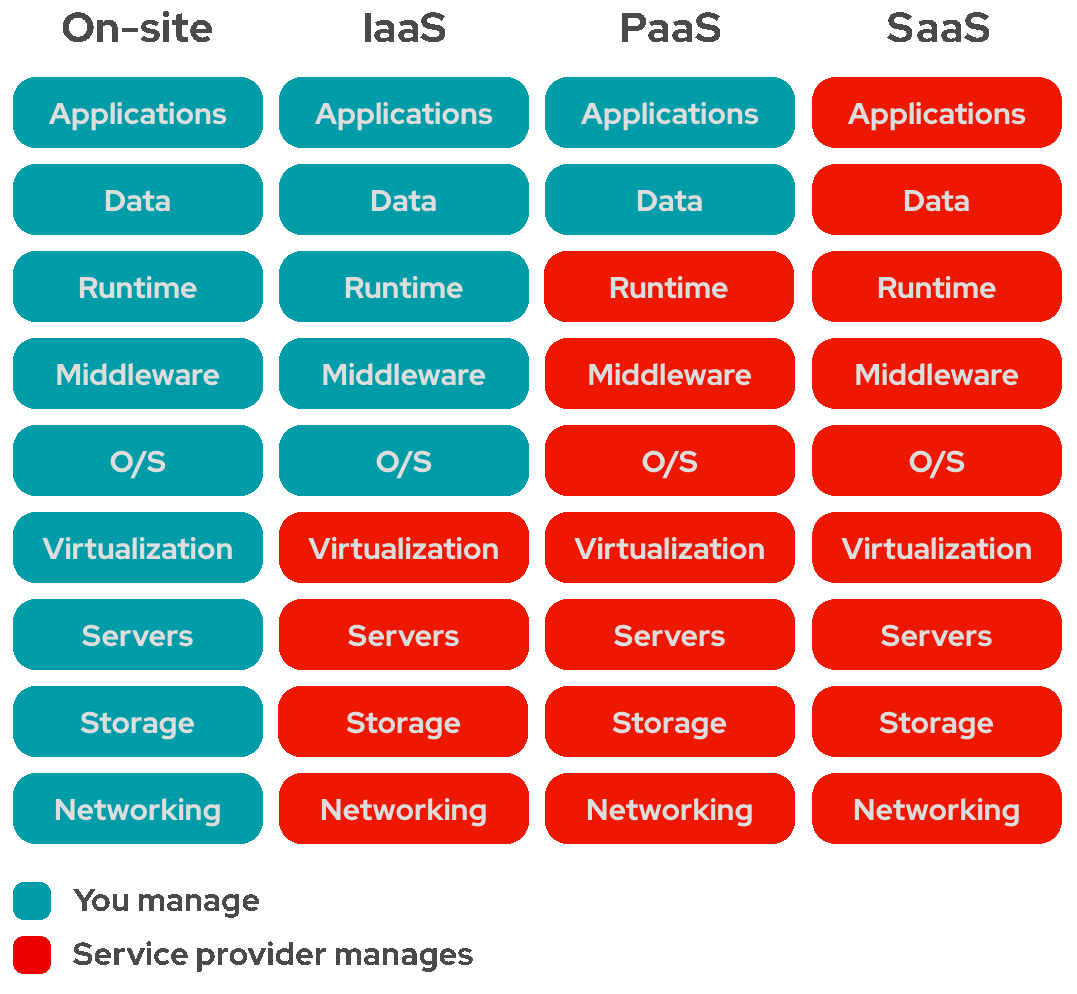
\includegraphics[width=.6\linewidth]{assets/2/cloud_level_services.png}
    \caption[Modelli di servizio fondamentali del cloud computing.]{Modelli di servizio fondamentali del cloud computing. Fonte: \url{https://www.redhat.com/en/topics/cloud-computing/iaas-vs-paas-vs-saas}}
    \label{fig:2_cloud_level_services}
\end{figure}

\subsection{Function as a Service}

Dalla nascita del cloud computing si sono evoluti nuovi paradigmi basati su esso, tra cui il serverless computing, definito in \cite{Castro2019} come una piattaforma che nasconde l'utilizzo del server agli sviluppatori ed esegue codice su richiesta in maniera automatica, scalabile e fatturata solo per il tempo effettivo di esecuzione. All'interno di questo modello sono presentati due approcci: Backend as a Service (BaaS), in cui la piattaforma eroga servizi di base, come la gestione dei database o dell'autenticazione, esponendo delle API che gli sviluppatori integrano per costruire le applicazioni; e Function as a Service (FaaS), di principale interesse per lo studio presentato in questa tesi.

L'approccio FaaS consente agli sviluppatori la creazione di applicazioni come insieme di funzioni, senza dover gestire l'infrastruttura necessaria per la loro esecuzione. Ogni funzione è specializzata un compito specifico ed è considerata come l'unita minima di esecuzione. L'infrastruttura FaaS è costituita da un modello di esecuzione ad eventi, in cui le funzioni sono:

\begin{itemize}
    \item Senza stato (stateless), per cui non viene mantenuta alcuna informazione con le esecuzioni precedenti,

    \item Temporanee, poiché le funzioni solo le risorse computazionali solo durante la loro esecuzione,

    \item Invocate da eventi, e quindi senza un processo costantemente attivo in attesa,

    \item Gestite dalla piattaforma, in cui lo sviluppatore è tariffato solo per le risorse utilizzate e le invocazioni.
\end{itemize}

Poiché le funzioni sono senza stato e basate su eventi, risultano facilmente scalabili in tempo reale in base al numero di richieste, poiché la piattaforma crea (o distrugge) delle copie in parallelo che si adattano per soddisfare la domanda.

La natura serverless di FaaS presenta vantaggi e svantaggi. Se FaaS permette a sviluppatori di accelerare lo sviluppo e alleggerire la gestione dell'infrastruttura, il modello non è pensato per l'esecuzione di funzioni per un lungo periodo di tempo. Inoltre FaaS soffre del problema ``cold start'': nel momento in cui una funzione viene invocata infatti, la piattaforma verifica la presenza di un’istanza pronta per eseguirla, ma nel caso in cui non esistesse allora ne viene avviata una nuova e ciò causa un aumento dei tempi di risposta, causando potenziali disagi agli applicativi che richiedono latenze contenute \cite{Ana2024}.

Ogni grande piattaforma di cloud computing offre un servizio FaaS, come Microsoft Azure Functions\footnote{\url{https://azure.microsoft.com/it-it/products/functions/}} o AWS Lambda\footnote{\url{https://aws.amazon.com/it/lambda/}}. Esistono inoltre implementazioni open source del modello FaaS, come Fission\footnote{\url{https://fission.io/}} e OpenFaaS\footnote{\url{https://www.openfaas.com/}}, di cui \Cref{fig:2_openfaas} ne mostra l'architettura dal punto di vista del gestore della piattaforma.

\begin{figure}
    \centering
    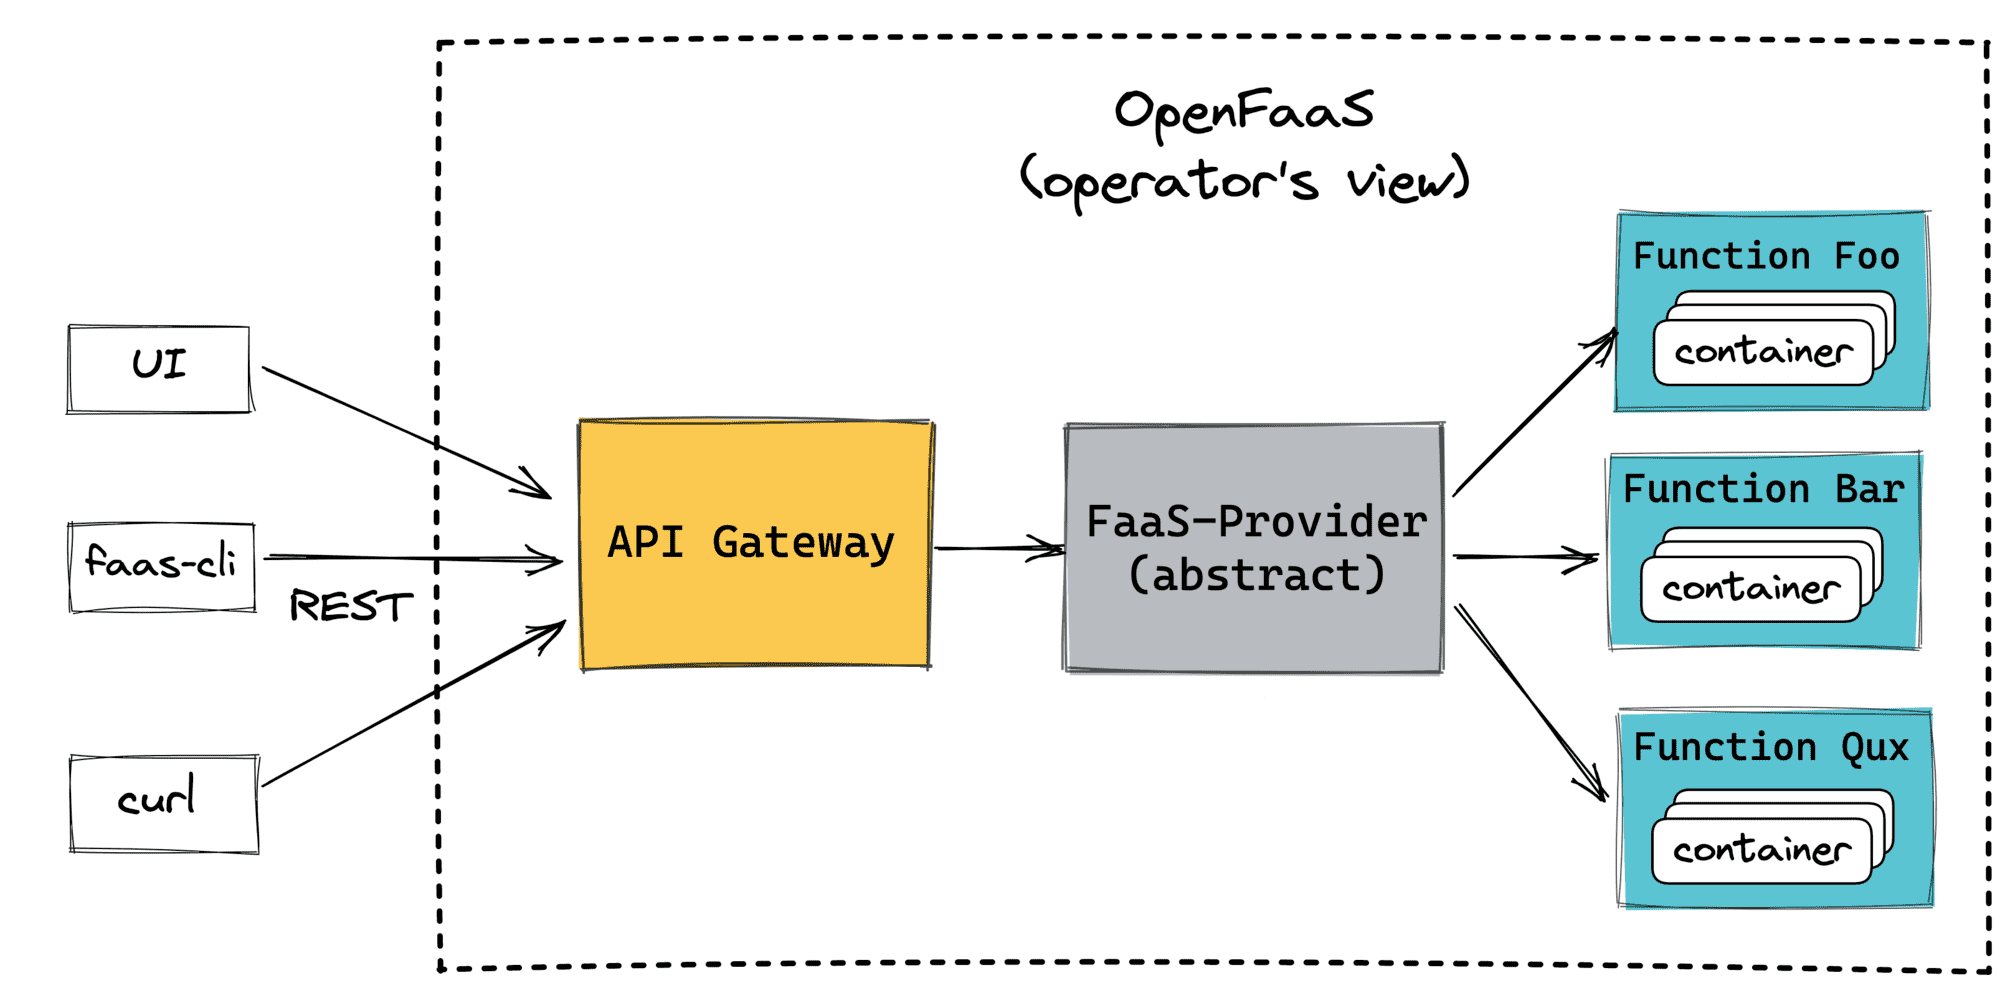
\includegraphics[width=0.8\linewidth]{assets/2/openfaas.png}
    \caption[Architettura generale di una piattaforma FaaS]{Architettura generale una piattaforma FaaS, nello specifico OpenFaaS. Fonte: \url{https://iximiuz.com/en/posts/openfaas-case-study/}}
    \label{fig:2_openfaas}
\end{figure}

\subsection{Edge computing}

Negli ultimi anni, il mondo dell'Internet of Things (IoT) ha vissuto uno sviluppo senza precedenti, con un aumento dei dispositivi e di connessioni che ha comportato una grande crescita nella produzione di dati, come si evince in \cite{Duarte2024}. L'analisi di questi dati può rivelarsi uno strumento importante, ma richiede una grande capacità computazionale in un unico preciso punto della rete. Sebbene il cloud computing possa essere utilizzato per questi scopi, ci sono delle limitazioni sulla possibilità di elaborare una tale quantità di dati, soprattutto se bisogna soddisfare richieste di utenti in termini di Qualità del Servizio (QoS), come esplicitato in \cite{Laroui2021}.

Per far fronte a queste necessità sono nati nuovi paradigmi denominati fog ed edge computing, presentati in modo più approfondito in \cite{Hurbungs2021}, il cui obiettivo principale è quello di spostare la computazione dal centro ai margini della rete. I vantaggi sono molteplici: consente di ridurre la latenza rispetto alla computazione presente al centro della rete, oltre a poter progettare una computazione suddivisa sui diversi livelli: le informazioni di minor valore possono infatti essere individuate e scartate ai bordi della rete, mentre i dati più importanti possono essere inoltrati al cloud per l’elaborazione definitiva. Si possono gestire all'edge dati che non possono essere mandati al cloud per questione di privacy, oppure perché sono richieste analisi in tempo reale che non sono compatibili con i ritardi che verrebbero introdotti con il cloud.

Se nel fog computing avviene la decentralizzazione di un’infrastruttura di elaborazione tramite ampliamento del cloud, attraverso il posizionamento strategico di nodi tra il cloud e i dispositivi terminali, nell'edge computing questo processo è portato all'estremo. Nell'edge computing la computazione è situata nei nodi periferici della rete, risultando, di conseguenza, più prossima all'utente finale e al luogo di generazione dei dati. La \Cref{fig:2_cloud_fog_edge} mostra la differenza dei tre modelli.

\begin{figure}
    \centering
    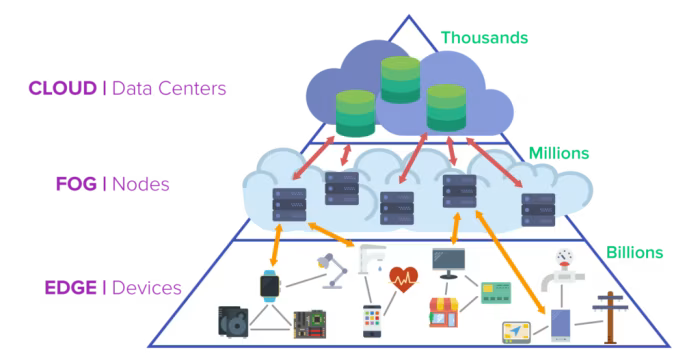
\includegraphics[width=.8\linewidth]{assets/2/cloud_fog_edge.png}
    \caption[Differenze tra cloud, fog ed edge computing]{Differenze tra cloud, fog ed edge computing. Fonte: \url{https://www.pubnub.com/blog/extending-cloud-technologies-to-the-edge/}}
    \label{fig:2_cloud_fog_edge}
\end{figure}

L'edge computing presenta diversi vantaggi: una minore latenza e maggiore velocità, dovuti dalla prossimità della computazione all'utente, riduzione dei costi ottimizzando il flusso dei dati verso i sistemi centrali, e infine una maggiore privacy e affidabilità, per via dell'elaborazione in loco.

\subsection{Decentralized FaaS}
\label{sec:2_dfaas}

Il paradigma FaaS convenzionale non è applicabile in un ambiente di edge computing, a causa del traffico dinamico e delle risorse computazionali limitate presenti sui nodi edge. Per poter mantenere i vantaggi di FaaS in tale ambiente è necessario quindi federare i nodi in ambienti di esecuzione distribuiti per bilanciare il carico tra di essi mediante la realizzazione di appositi algoritmi. Decentralized FaaS (DFaaS), introdotto in \cite{Ciavotta2021}, rappresenta proprio questo punto di unione tra i due modelli: l'architettura prevede degli ambienti federati e centralizzati in cui i nodi edge bilanciano automaticamente il traffico tra i nodi appartenenti a ecosistemi FaaS edge federati.

DFaaS utilizza una rete peer-to-peer overlay per scambiare dati sulla struttura della rete, tempi di risposta e capacità di carico dei nodi. Con l’espressione peer-to-peer si intende una rete formata da nodi connessi tra loro, che non hanno una gerarchia, ma sono equipotenti, o peer (pari). In linea generale, all'interno di questa architettura i nodi sovraccarichi utilizzano le informazioni scambiate nella rete per indirizzare alcune delle richieste di esecuzione FaaS ai nodi meno congestionati.

Lo scenario di riferimento di DFaaS, mostrato in \Cref{fig:2_dfaas_scenario}, consiste in una rete di nodi FaaS posti ai margini della rete e geograficamente distribuiti. In ciascun nodo è situata una piattaforma FaaS che esegue le funzioni serverless, tipicamente sotto forma di richieste HTTP, e per ciascun nodo è associato un punto di accesso per la connessione di rete. Di solito, uno o più nodi edge vengono gestiti da un edge provider, che potrebbe essere, ad esempio, un operatore di rete. I nodi possono appartenere al medesimo fornitore o a fornitori diversi e sono interconnessi tramite connessioni di rete, spesso regolate da accordi di livello di servizio (Service Level Agreement, SLA). L’ambiente descritto rappresenta un ecosistema federato di edge computing, in cui edge provider diversi, ciascuno con la propria piattaforma DFaaS e tecnologie specifiche, si uniscono in federazione. Così facendo, possono sfruttare in modo trasparente le risorse computazionali offerte dai nodi edge di altri fornitori. Questa collaborazione diventa particolarmente rilevante quando i nodi sperimentano un sovraccarico dovuto a picchi di traffico. 

\begin{figure}
    \centering
    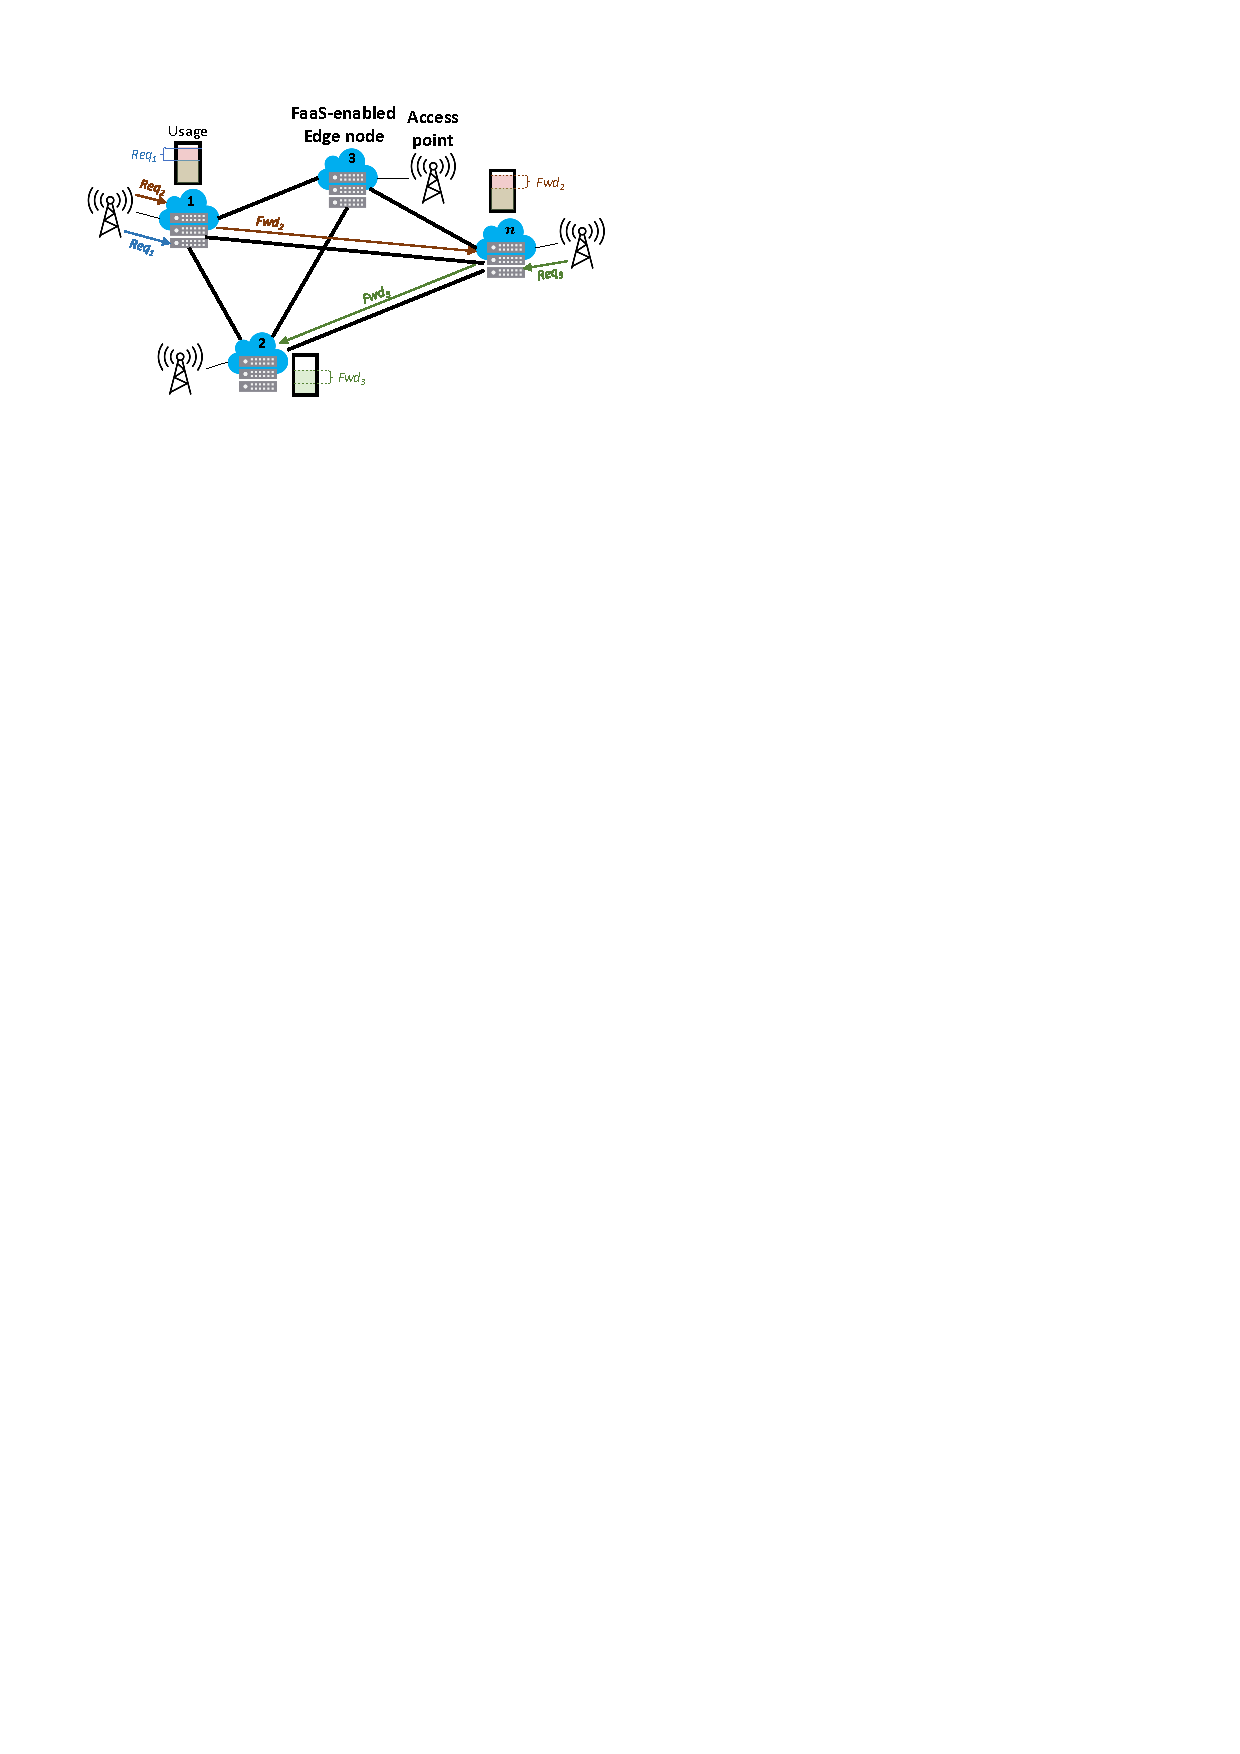
\includegraphics[width=.7\linewidth]{assets/2/dfaas_scenario.pdf}
    \caption[Scenario di riferimento di DFaaS]{Scenario di riferimento di DFaaS in \cite{Ciavotta2021}}
    \label{fig:2_dfaas_scenario}
\end{figure}

L'architettura di DFaaS è mostrata in \Cref{fig:2_dfaas_architecture}: si avvale di componenti consolidate, attivamente mantenute e testate, ponendo un'enfasi particolare sulla modularità, manutenibilità ed evolvibilità della piattaforma.

\begin{figure}
    \centering
    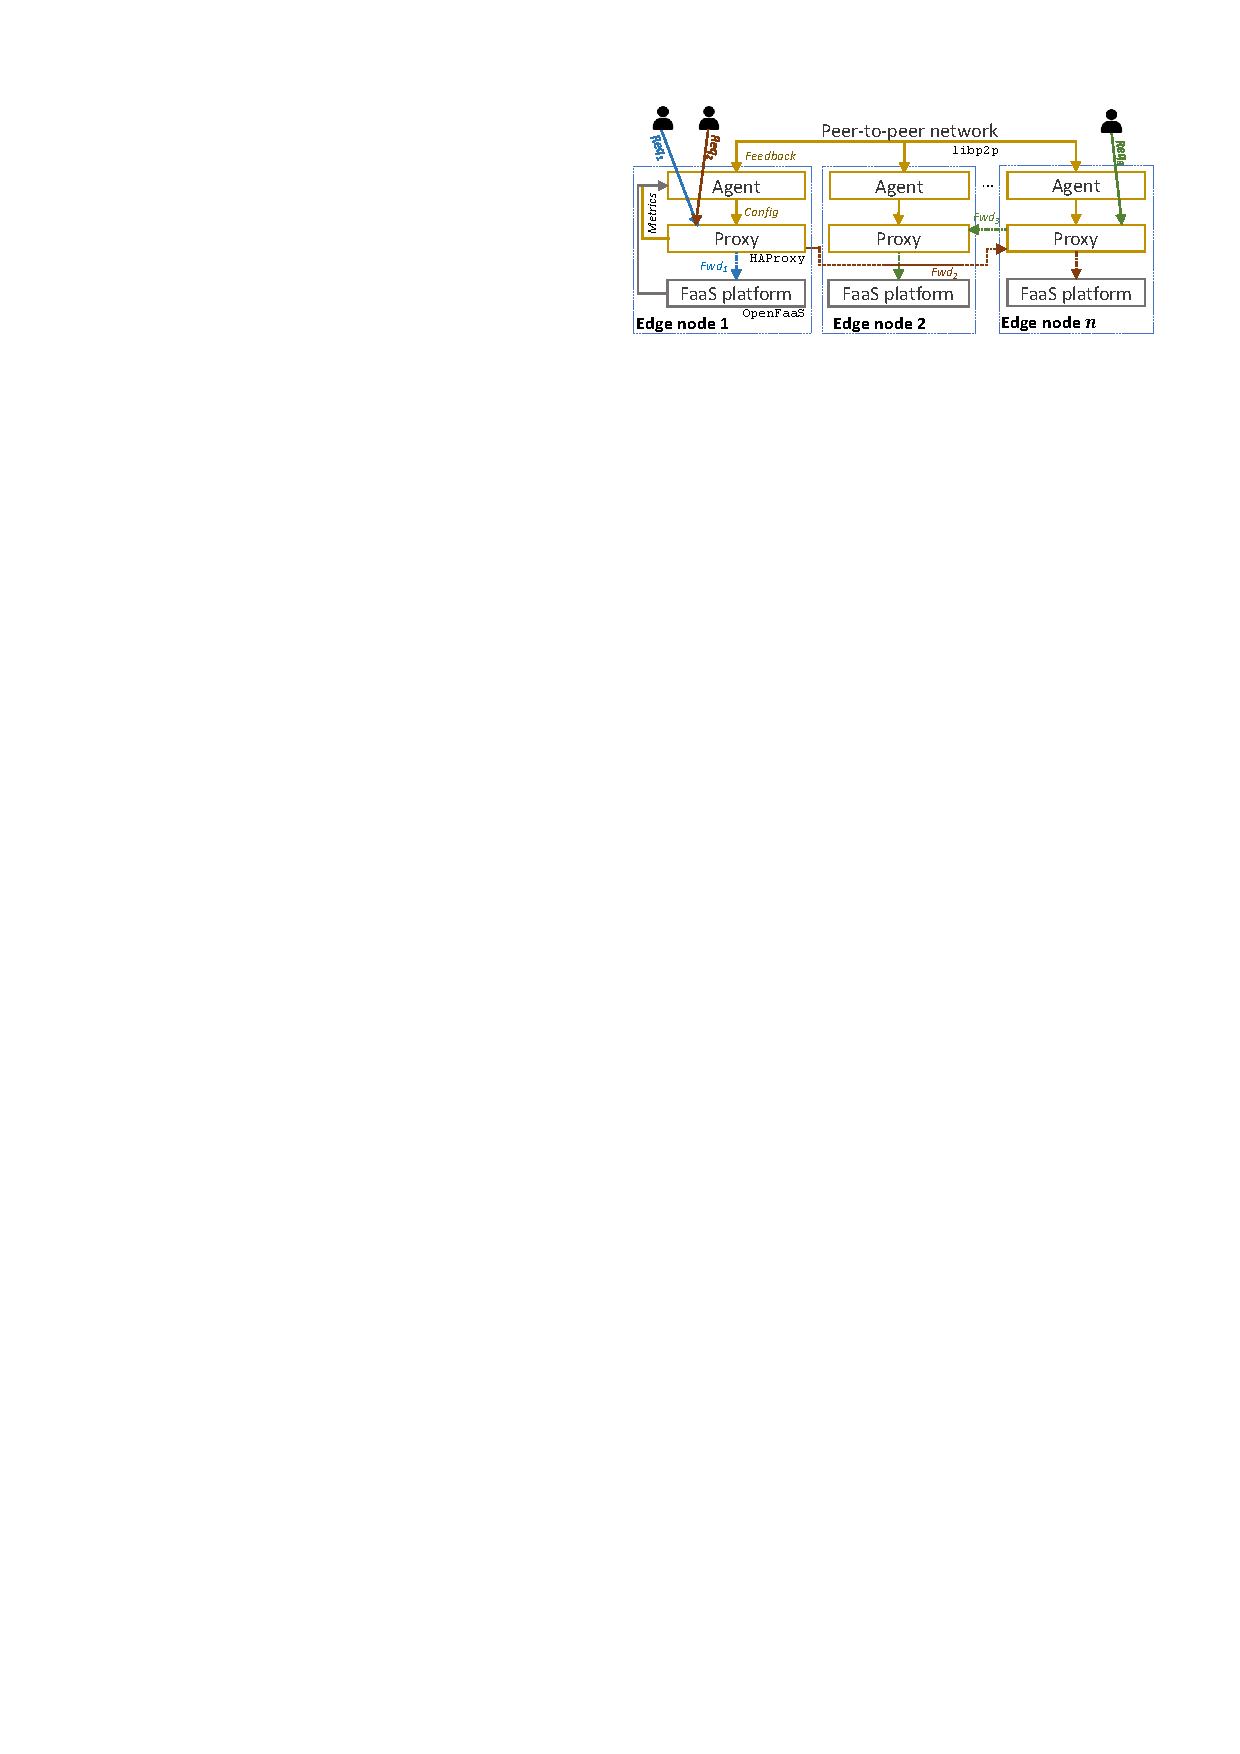
\includegraphics[width=.7\linewidth]{assets/2/dfaas_architecture.pdf}
    \caption[Architettura di DFaaS]{Architettura di DFaaS in \cite{Ciavotta2021}}
    \label{fig:2_dfaas_architecture}
\end{figure}

I principali componenti, replicati su tutti i nodi, sono:

\begin{itemize}
    \item Agenti: ogni agente è responsabile di gestire la connessione alla rete peer-to-peer e la comunicazione con gli altri agenti. Monitora periodicamente lo stato della piattaforma FaaS sul nodo in cui si trova, raccogliendo metriche pertinenti alle capacità computazionali disponibili. Configura il proxy per fare in modo di reindirizzare il traffico ai nodi previsti in base agli accordi che può negoziare con gli altri agenti. 

    \item Proxy: si occupa di gestire le richieste HTTP in ingresso, inoltrandole alla piattaforma FaaS locale oppure a un altro nodo edge. In DFaaS è implementato attraverso HAProxy\footnote{\url{https://www.haproxy.org/}}.  

    \item Piattaforma FaaS: si occupa di eseguire sul nodo locale la funzione invocata, allocando le risorse computazionali necessarie. DFaaS utilizza OpenFaaS.
\end{itemize}

Tale modello è stato considerato come l'obiettivo da replicare nello studio in questione, ponendo alcune semplificazioni per realizzare un ambiente simulato che tuttavia rispecchi gli aspetti caratteristici di DFaaS. Nel \Cref{sec:4_modellazione} verrà presentata la modellazione di DFaaS.

\section{Apprendimento per Rinforzo}

L'Apprendimento per Rinforzo (Reinforcement Learning, abbreviato RL) è un'area interdisciplinare del machine learning e del controllo che riguarda l'adattamento e l'ottimizzazione del comportamento di un agente all'interno di un ambiente dinamico, al fine di massimizzare una ricompensa cumulativa \cite{Sutton2018}. I componenti fondamentali in un sistema di RL sono i seguenti, mostrati anche in \Cref{fig:2_rl_components}:

\begin{itemize}
    \item Agente: è l'entità che sceglie le azioni,

    \item Ambiente: è il contesto in cui l'agente interagisce e su cui hanno effetto le azioni intraprese,

    \item Ricompensa: è un segnale numerico che quantifica la qualità di un'azione, allo scopo di incoraggiare la scelta di azioni corrette.
\end{itemize}

\begin{figure}
    \centering
    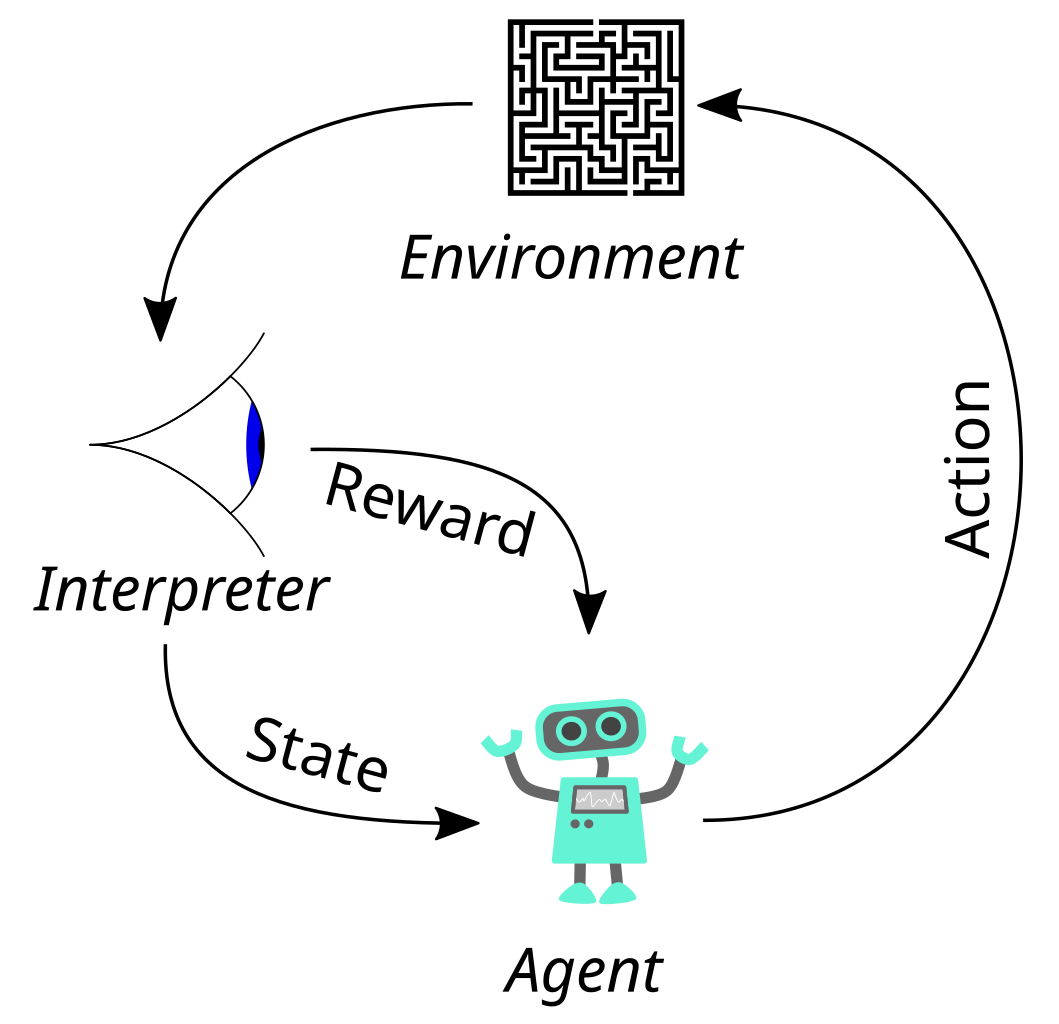
\includegraphics[width=.5\linewidth]{assets/2/rl_components.png}
    \caption[Componenti tipici in un sistema RL]{Componenti tipici in un sistema RL. Un agente prende decisioni in base all'osservazione (lo stato), tale azione produce delle conseguenze sull'ambiente che sono valutate e viene restituito il feedback all'agente, insieme al nuovo stato. Fonte: Megajuice, CC0, Wikimedia Commons.}
    \label{fig:2_rl_components}
\end{figure}

Un aspetto importante di un sistema RL è che all'agente non viene indicato quale azione deve intraprendere, bensì è l'agente stesso a scoprire in autonomia come agire per massimizzare la ricompensa sul lungo periodo. Nei casi più interessanti e complessi, le azioni possono influenzare non solo la ricompensa immediata, ma anche gli stati futuri del sistema e, attraverso questi, le ricompense future. L'apprendimento per tentativi ed errori e la ricompensa ritardata sono tra le due caratteristiche distintive dell'apprendimento per rinforzo. 

Un problema RL viene formalizzato come un un processo decisionale di Markov, approfondito nella \Cref{sec:2_mdp}, con l'obiettivo di trovare una policy\footnote{Una strategia che l'agente segue, definita nella \Cref{sec:2_rl_functions}.} ottimale per il processo, senza che l'agente sia a conoscenza dell'evoluzione del processo e di come vengono calcolate le ricompense. Tali processi possono essere risolti utilizzando algoritmi di programmazione dinamica\footnote{Tecnica in cui si semplifica un problema in sotto-problemi più semplici in modo ricorsivo.}. Tuttavia, questi richiedono di sviluppare un modello, con le difficoltà associate. Gli algoritmi RL invece non ipotizzano di conoscere esattamente il modello matematico, e possono quindi essere usati con modelli di grandi dimensioni che altrimenti sarebbero intrattabili con i metodi classici.

Un punto importante degli algoritmi RL è trovare un bilanciamento tra l'esplorazione (di un territorio inesplorato) e lo sfruttamento (dell'esperienza accumulata) con l'obiettivo di massimizzare la ricompensa nel lungo periodo, poiché  in cui il riscontro delle scelte può essere incompleto o ritardato. Il bilanciamento è importante perché un'eccessiva esplorazione può portare a perdere opportunità di ottenere ricompensa da azioni note, mentre un eccessivo sfruttamento può impedire all'agente la scoperta di nuove azioni più fruttuose.

\paragraph{Differenze tra RL e altri metodi.} Il RL si differenzia dall'apprendimento supervisionato, poiché RL non richiede un insieme di esempi etichettati ed è in grado di apprendere in contesti dinamici. Un'altra differenza riguarda la sparsità del feedback: il feedback che riceve un agente può non essere informativo finché l'ambiente non raggiunge un determinato stato. Infine c'è una differenza anche nella generazione dei dati, in cui nell'apprendimento supervisionato avviene in modo indipendente dall'algoritmo, mentre nel RL viene generato dall'agente che interagisce con l'ambiente.

Il RL si differenzia anche dall'apprendimento non supervisionato, perché ha come obiettivo la massimizzazione della ricompensa nel lungo periodo e non l'identificazione di strutture nascoste nei dati. Per questi motivi il RL è considerato come un paradigma a sé stante nel campo del machine learning.

\paragraph{} Di seguito verranno introdotti alcuni concetti essenziali del RL per comprendere al meglio le scelte e le tecniche usate per modellazione e applicazione di algoritmi del caso di studio. Per un quadro d'insieme introduttivo più ampio è possibile consultare \cite{Ghasemi2024}.

\subsection{Processo decisionale di Markov}
\label{sec:2_mdp}

Un processo decisionale di Markov (Markon Decision Process, MDP) è un modello decisionale che opera in modo sequenziale, con tempi definiti in passi discreti \cite{Puterman1994}. Un MDP è definito come una quadrupla $(\mathcal{S}, \mathcal{A}, \mathcal{P}, \mathcal{R})$:

\begin{itemize}
    \item $\mathcal{S}$ è l'insieme finito degli stati,

    \item $\mathcal{A}$ è l'insieme finito delle azioni,

    \item $\mathcal{P}$ è la funzione di probabilità di transizione tra gli stati, definita come ${\mathcal{P}: \mathcal{S} \times \mathcal{A} \times \mathcal{S} \to [0, 1]}$ per cui

    \begin{equation}
        \forall s \in \mathcal{S}, a \in \mathcal{A}: \sum_{s' \in \mathcal{S}} \mathcal{P}(s, a, s') = 1,
    \end{equation}

    \item $\mathcal{R}$ è la funzione di ricompensa, definita come $\mathcal{R}: \mathcal{S} \times \mathcal{A} \times \mathcal{S} \to \mathbb{R}$.
\end{itemize}

È importante sottolineare che gli agenti non hanno conoscenza delle funzioni di transizione $\mathcal{P}$ e di ricompensa $\mathcal{R}$, ma solo degli spazi delle azioni $\mathcal{A}$ e degli stati $\mathcal{S}$.

L'interazione tra l'agente e l'MDP produce una sequenza di esperienze, chiamata traiettoria e indicata come $\tau$, contenente la sequenza temporale di stati, azioni e ricompense incontrate dall'agente. La singola esperienza al passo $t$ è definita come una quadrupla $(s_t, a_t, r_t, s_{t+1})$, in cui

\begin{itemize}
    \item $s_t \in \mathcal{S}$ è lo stato dell'ambiente al passo $t$,

    \item $a_t \in \mathcal{A}$ è l'azione scelta dall'agente al passo $t$,

    \item $s_{t+1} \in \mathcal{S}$ è lo stato in cui l'ambiente si muove a seguito dell'azione $a_t$, scelta nello stato $s_t$ al passo $t$,

    \item $r_t = \mathcal{R}(s_t, a_t, s_{t+1})$ è la ricompensa ottenuta al passo $t$. \label{sec:2_reward_function_def}
\end{itemize}

Un esempio di MDP è mostrato in \Cref{fig:2_rl_mdp_example}.

\begin{figure}
    \centering
    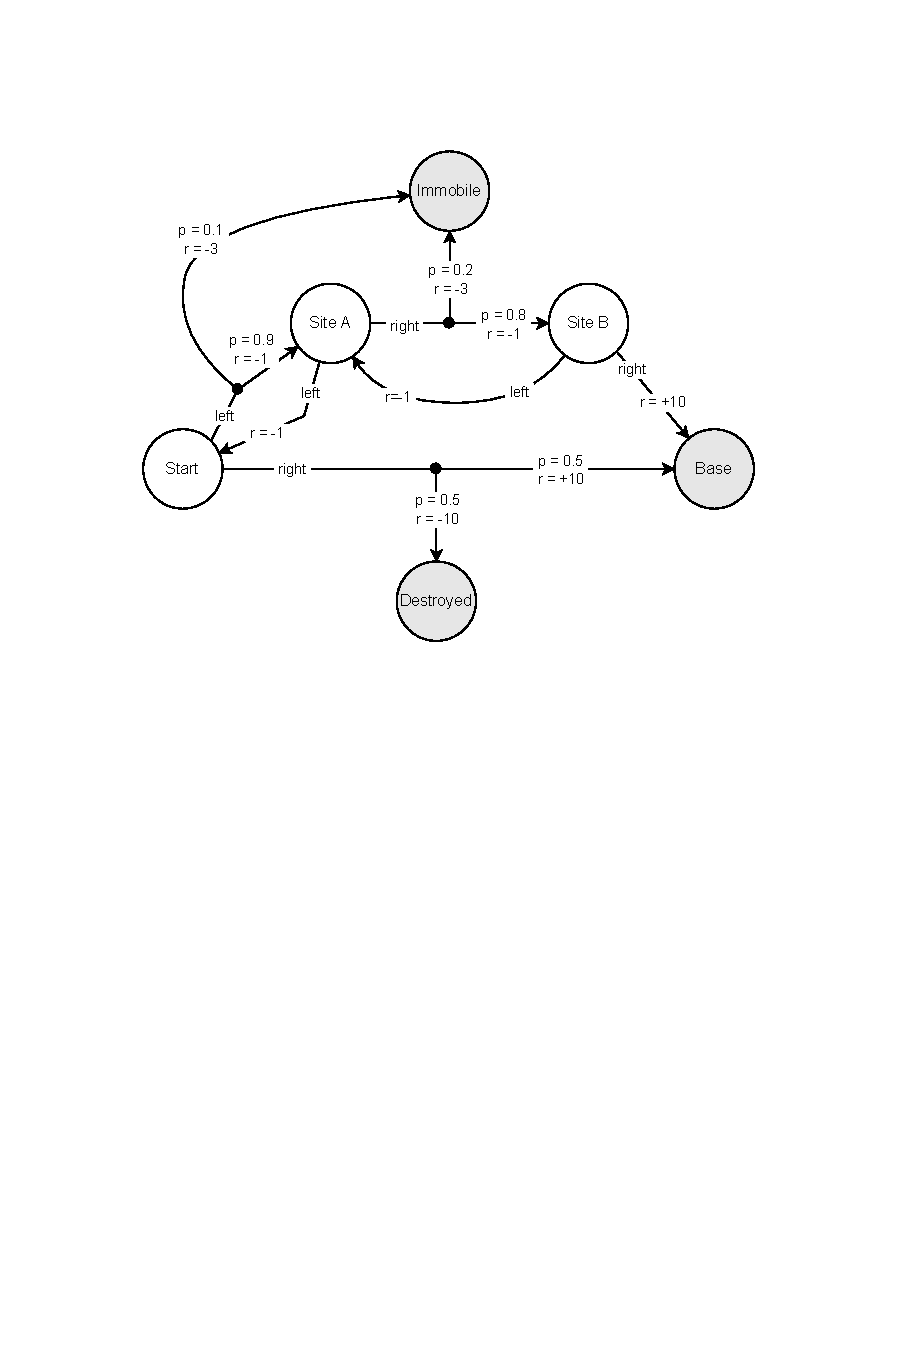
\includegraphics[width=.6\linewidth]{assets/2/rl_mdp_example.pdf}
    \caption[Esempio di un processo decisionale di Markov]{Esempio di un processo decisionale di Markov che modella il movimento di un rover su Marte. I cerchi sono gli stati, di cui quelli scuri sono terminali. A ogni stato sono associate due possibili azioni, destra e sinistra, mostrati come archi con la probabilità di transizione associata e la ricompensa. Fonte: \cite{Stefano2024}}
    \label{fig:2_rl_mdp_example}
\end{figure}

\paragraph{Proprietà di Markov.} Un MDP soddisfa la proprietà di Markov, da cui viene il nome: dato lo stato e la ricompensa attuale, lo stato e la ricompensa futuri non sono condizionati dagli stati e azioni passate, cioè:

\begin{equation}
    \mathbb{P}(s_{t+1}, r_t | s_t, a_t, s_{t-1}, \dots, s_0, a_0) = \mathbb{P}(s_{t+1}, r_t | s_t, a_t).
\end{equation}

Ne consegue che lo stato corrente fornisce le informazioni sufficienti per scegliere un'azione ottimale in un MDP, e che gli stati e azioni del passato non sono rilevanti.

\paragraph{Guadagno atteso scontato.} Data una traiettoria, il guadagno è la somma delle ricompense ottenute. Per via della natura stocastica di un MDP, non è possibile per l'agente massimizzare il guadagno per tutte le traiettorie, bensì l'obiettivo dell'agente è massimizzare il guadagno atteso per qualsiasi traiettoria, definito come:

\begin{equation}\label{eq:2_discounted_return}
    \mathbb{E} \left[ r_0 + \gamma r_1 + \gamma^2 r_2 + \dots \right] = \mathbb{E} \left[ \sum_{t=0}^{\infty} \gamma^t r_t \right].
\end{equation}

Poiché una traiettoria può essere infinita, per ottenere un valore atteso finito viene introdotto il fattore di sconto $\gamma \in [0, 1]$. Con un valore vicino a 0 le ricompense future avranno poca importanza, mentre vicino a 1 saranno considerate rilevanti. L'\Cref{eq:2_discounted_return} viene chiamata \textit{guadagno atteso scontato}.

\paragraph{MDP episodici e continui.} Una traiettoria in un MDP come presentato è infinita, poiché non esiste il concetto di stato terminale. MDP di questa tipologia si chiamano \textit{continui} o \textit{non-episodici}. Nonostante esistano definizioni di modelli più avanzati di MDP che introducono stati terminali, si può realizzare lo stesso concetto con un MDP: uno stato che una volta raggiunto rimane nello stesso stato, qualsiasi sia l'azione scelta dall'agente. Questa tipologia di MDP si chiama \textit{episodica}, perché ha una durata limitata di numero di interazioni, o \textit{passi}.

\subsection{Funzioni fondamentali}
\label{sec:2_rl_functions}

In un sistema di RL l'obiettivo dell'agente è massimizzare il guadagno atteso scontato. Per raggiungere questo scopo, l'agente può imparare una delle tre funzioni primarie:

\begin{itemize}
    \item Policy: è la strategia che l'agente segue per prendere una decisione a partire da uno stato. Una policy $\pi$ è tipicamente stocastica, pertanto è definita come

    \begin{equation}
        \pi: \mathcal{A} \times \mathcal{S} \to [0, 1], \qquad \pi(a, s) \coloneqq \mathbb{P}(a_t = a | s_t = s)
    \end{equation}
    
    e si indica come $a \sim \pi(s)$ l'azione $a$ estratta dalla policy $\pi$ per lo stato $s$.
    
    La policy $\pi$ esprime quindi la probabilità di scegliere un'azione a partire da uno stato, e può essere rappresentata mediante una funzione, una tabella o, in scenari più complessi, attraverso modelli stocastici o reti neurali.
    
    Esistono anche policy deterministiche, in cui dato uno stato viene scelta sempre la stessa azione, ma sono meno comunemente applicate rispetto alle policy stocastiche perché quest'ultime si adattano in scenari con una grande varianza nelle dinamiche di transizione.

    \item Funzione di valore e valore-azione: sono due funzioni strettamente collegate, in cui

    \begin{itemize}
        \item Funzione di valore: quantifica il guadagno atteso a partire da uno stato $s$, ipotizzando che l'agente continui a operare con la stessa policy $\pi$. Rappresentata in letteratura come $V^\pi$, è definita come:

        \begin{equation}
            V^\pi: \mathcal{S} \to \mathbb{R}, \qquad V^\pi(s) \coloneqq \mathbb{E}_{s_0=s, \tau \sim \pi} \left[ \sum_{t=0}^{\infty} \gamma^t r_t\right].
        \end{equation}
    
        Questo concetto permette di valutare l’efficacia di una sequenza di azioni nel lungo termine, anche quando alcune di queste possono sembrare inizialmente sconvenienti.

        \item Funzione Valore-Azione: quantifica il guadagno atteso scegliendo un'azione $a$ da uno stato $s$, ipotizzando che l'agente continui in seguito a operare con la stessa policy $\pi$. Rappresentata in letteratura come $Q^\pi$, è definita come

        \begin{equation}
            Q^\pi: \mathcal{S} \times \mathcal{A} \to \mathbb{R}, \qquad Q^\pi(s, a) \coloneqq \mathbb{E}_{s_0=s, a_0=a, \tau \sim \pi} \left[ \sum_{t=0}^{\infty} \gamma^t r_t\right].
        \end{equation}
    \end{itemize}
    
    \item Modello dell'ambiente: l'agente impara un modello delle dinamiche di transizione osservate come una funzione $P(s' | s, a)$, e utilizza tale modello per prevedere la sequenza della azioni e stati futuri permettendo quindi di selezionare l'azione migliore. 
\end{itemize}

\subsubsection{Ottimalità}

L'obiettivo primario quando si affronta un problema di RL è identificare o approssimare una policy ottimale. Una policy $\pi$ è considerata ottimale se, per ogni stato possibile, massimizza il valore atteso del guadagno rispetto a tutte le altre policy.

Formalmente, una policy $\pi$ è ottimale rispetto a un'altra policy $\pi'$ se

\begin{equation}
    \forall s \in \mathcal{S}: V^\pi(s) \ge V^{\pi'}(s).
\end{equation}

La policy ottimale, denotata come $\pi^\ast$, è strettamente legata alle funzioni di valore ottimale, $v^\ast(s)$, e di azione-valore ottimale, $q^\ast(s, a)$. Queste funzioni rappresentano il massimo guadagno atteso che un agente può ottenere da uno stato o da una coppia stato-azione, seguendo la policy ottimale:

\begin{equation}
    v^*(s) \coloneqq \max_\pi V^\pi(s) \quad \forall s \in \mathcal{S},
\end{equation}

\begin{equation}
    q^*(s, a) \coloneqq \max_\pi Q^\pi(s, a) \quad \forall s \in \mathcal{S}, \forall a \in \mathcal{A}.
\end{equation}

\subsubsection{Metodi fondamentali}

Esistono tre metodologie di base che permettono di apprendere strategie ottimali attraverso l'interazione con l'ambiente. Le idee alla base dei seguenti metodi sono state riprese dagli algoritmi più moderni e avanzati. I tre metodi sono i seguenti:

\begin{itemize}
    \item Programmazione dinamica (dynamic programming, DP): il metodo utilizza le equazioni ricorsive di Bellman per trovare la policy ottimale e i corrispondenti valori di stato ottimale. Utilizza due approcci iterati in sequenza: policy evaluation, in cui viene calcolata la funzione di valore, e policy improvement, in cui viene elaborata una policy migliore usando la funzione di valore.

    È un metodo efficace nel caso si conosca la struttura completa del MDP, perché produce delle soluzioni ottimali esatte. Tuttavia per modelli non noti o spazi di osservazioni e azioni estesi risulta impraticabile.

    \item Monte Carlo: sono dei metodi che non si basano sulla conoscenza del modello, acquisiscono esperienza direttamente dall'interazione con l'ambiente raccogliendola da traiettorie complete di episodi. Ogni traiettoria viene poi usata per aggiornare la funzione di valore. A causa della loro natura, possono convergere in soluzioni non ottimali, per questo motivo è necessario garantire l'esplorazione, tramite un'alternanza di stati iniziali oppure un'esplorazione forzata tramite azioni casuali.

    \item Apprendimento mediante differenza temporale (temporal difference learning, TD): questi metodi utilizzano l'esperienza diretta come Monte Carlo, ma con aggiornamenti incrementali della programmazione dinamica. In particolare, sono in grado di aggiornare le stime del valore di uno stato utilizzando le stime di stati successivi, permettendo così un apprendimento continuo e incrementale durante ogni episodio. Questo permette l'utilizzo di TD in ambienti non episodici.
\end{itemize}

\subsection{Tipologia di algoritmi}
\label{sec:2_rl_algorithms_types}

Un algoritmo di RL può basarsi sull'imparare la policy, la funzione di valore, il modello o una combinazione di questi; ciò ne caratterizza la tipologia:

\begin{itemize}
    \item Policy-based: sono algoritmi che imparano direttamente a costruire la policy $\pi$, tra cui quelle ottimali che sono le policy che massimizzano il guadagno atteso. Il vantaggio di questi algoritmi è che si adattano a spazi di azioni sia continui sia discreti, e inoltre ottimizzano direttamente il guadagno atteso. È dimostrato in \cite{Sutton2018} che algoritmi di questa tipologia convergono a una policy ottima locale. Lo svantaggio è che soffrono di grande varianza e richiedono molta esperienza per imparare.

    \item Value-based: sono algoritmi che imparano le funzioni $V^\pi$ o $Q^\pi$ per valutare uno stato e un'azione per generare una policy. Il vantaggio di questi algoritmi è che sono più efficienti di quelli policy-based perché richiedono meno esperienza e soffrono di meno varianza. Lo svantaggio è che non è garantito che tali algoritmi convergano in un ottimo e sono adatti solo a spazi di azioni discreti.

    \item Model-based: algoritmi di questa tipologia imparano un modello delle dinamiche di transizioni $P$ e utilizzano tale modello per scegliere l'azione migliore. Il vantaggio di questo approccio è che richiede meno esperienza per ottenere delle buone azioni ed è pertanto rapido nell'imparare. Lo svantaggio principale è che, in caso di un ambiente complesso e con dinamiche di transizioni elaborate, con spazi delle azioni e degli stati di dimensione elevata, costruire un modello può essere intrattabile. Un algoritmo che non costruisce un modello si denomina ``model-free''. 
\end{itemize}

\paragraph{On-policy e off-policy.} Un'ultima distinzione tra gli algoritmi di RL è data dall'esperienza con cui addestrano le funzioni fondamentali al fine di generare una policy. Algoritmi on-policy richiedono più esperienza raccolta, perché l'addestramento avviene, in ogni iterazione, con dati generati dalla policy $\pi$ nella medesima iterazione, scartando i dati al termine della stessa. Algoritmi off-policy al contrario non hanno questo vincolo e possono usare l'esperienza raccolta in qualsiasi fase dell'addestramento. Quest'ultimi richiedono di raccogliere esperienza in ogni iterazione, ma è necessaria più memoria per salvare i dati raccolti nel corso del processo di apprendimento.

\subsection{Sistemi multi-agente}

Lo scenario classico dell'apprendimento per rinforzo prevede un solo agente che interagisce con l'ambiente, tuttavia molti problemi possono essere modellati come più agenti che condividono lo stesso ambiente. Tali agenti possono interagire con l'ambiente in contemporanea, come nei casi reali di veicoli a guida autonoma, oppure a turni, come spesso accade nei giochi (scacchi, dama). Questo scenario costituisce un sistema di apprendimento per rinforzo multi-agente (multi-agent reinforcement learning, MARL).

La \Cref{fig:2_rl_multi_agent_schematic} mostra lo scenario di riferimento, che è analogo al caso di RL con singolo agente, esteso però su più agenti. Un vantaggio importante del MARL è che è possibile decomporre problemi complessi di decisione in sotto-problemi più piccoli, ognuno dei quali gestito da un singolo agente.

\begin{figure}
    \centering
    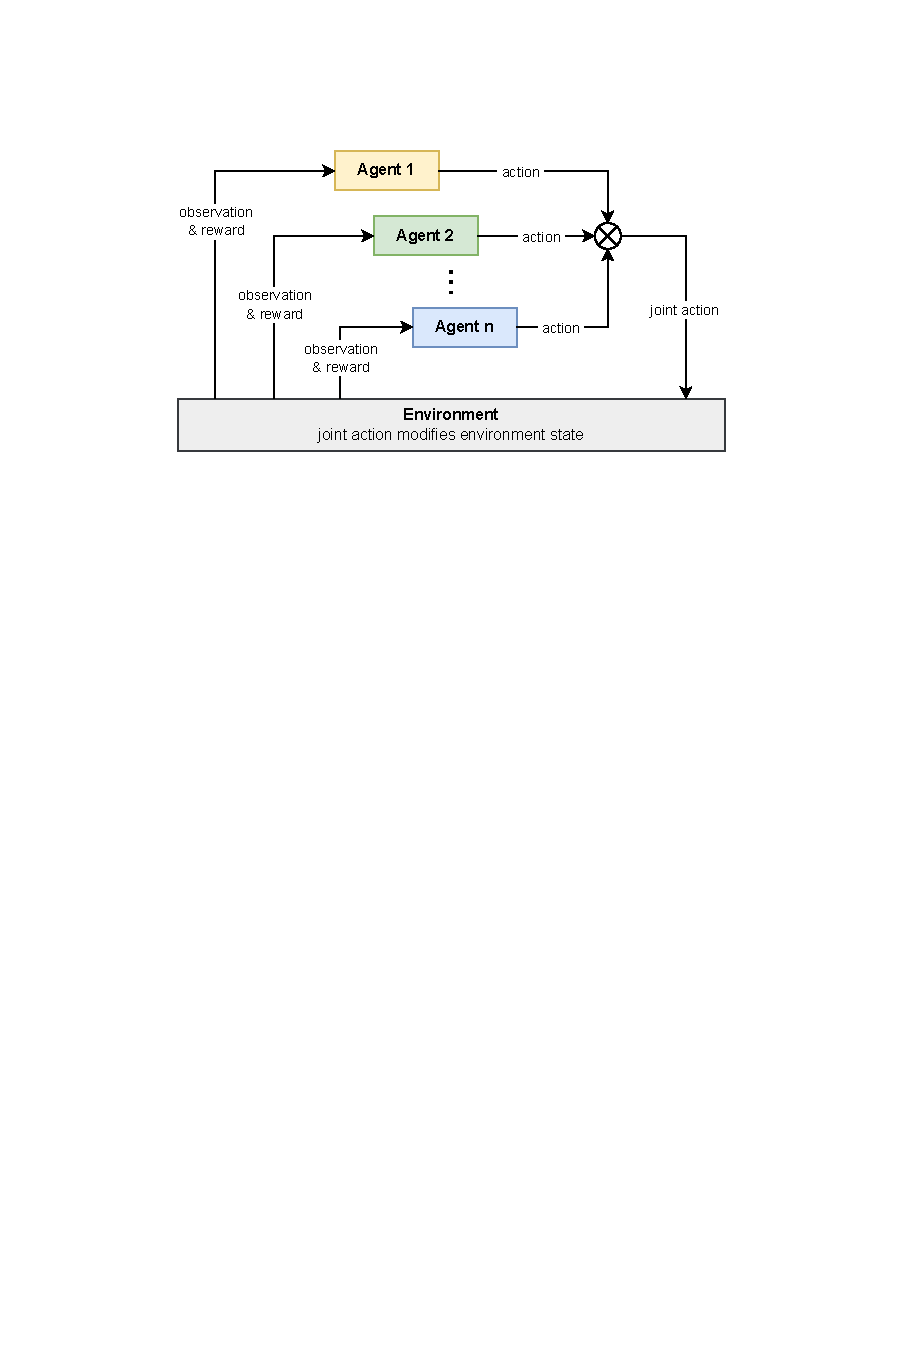
\includegraphics[width=0.7\linewidth]{assets/2/rl_multi_agent_schematic.pdf}
    \caption[Schematica dell'Apprendimento per Rinforzo multi-agente]{Schematica dell'Apprendimento per Rinforzo multi-agente, in cui un insieme di n agenti ricevono delle osservazioni individuali sullo stato dell'ambiente, e scelgono delle azioni per modificare lo stato. Ogni agente quindi riceve una ricompensa numerica e una nuova osservazione. Fonte: \cite{Stefano2024}}
    \label{fig:2_rl_multi_agent_schematic}
\end{figure}

\paragraph{Fasi di addestramento ed esecuzione.} In MARL la distinzione tra fase di addestramento e di esecuzione ha particolare importanza, perché permette di categorizzare gli approcci principali, approfonditi in \cite{Stefano2024}:

\begin{itemize}
    \item Addestramento ed esecuzione centralizzata: le due fasi avvengono in modo centralizzato, condividendo le informazioni disponibili su tutti gli agenti. Questo è l'approccio migliore per ottenere una buona coordinazione tra agenti, ma non tutti i problemi ammettono tale configurazione. Infatti, richiede di condividere le osservazioni e le decisioni, non sempre consentito per vincoli di privacy o comunque complesso in ambienti decentralizzati. 

    \item Addestramento ed esecuzione decentralizzata: non c'è una condivisione delle informazioni tra agenti in nessuna fase, ogni agente impara ed esegue azioni solo in base alle proprie osservazioni. Un importante limite di questo approccio è che l'ambiente non è più stazionario, violando pertanto la proprietà di Markov: le transizioni e la ricompensa non dipendono più soltanto dallo stato corrente. 

    \item Addestramento centralizzato, esecuzione decentralizzata: mira a equilibrare i due metodi, assumendo che sia possibile centralizzare l'addestramento (per esempio con una simulazione) mentre l'esecuzione avviene in modo completamente decentralizzato.
\end{itemize}

\paragraph{Cooperazione o collaborazione.} In uno scenario MARL gli agenti possono avere interessi diversi tra loro: si figurano dunque scenari competitivi, in cui gli interessi degli agenti sono contrapposti, scenari collaborativi, in cui gli interessi sono gli stessi, o scenari misti.

\subsection{Approccio Deep Learning}

Il Deep Reinforcement Learning (DRL) rappresenta un ramo dell'apprendimento per rinforzo che fonde il RL e il Deep Learning. Algoritmi di questa tipologia utilizzano le reti neurali per l'addestramento dell'agente, approssimando le funzioni di valore $V^\pi$ o $Q^\pi$, le politiche $\pi$ o il modello $P$.

Rispetto all'apprendimento supervisionato, nel DRL l'input e l'output per le reti neurali non sono fornite in anticipo, bensì i dati sono ottenuti dall'interazione tra l'agente e l'ambiente. La generazione dei dati e la valutazione dei risultati presenta inoltre difficoltà aggiuntive, poiché la funzione che la rete neurale impara è strettamente legata all'MDP: lo scambio di dati tra l'agente e l'ambiente è interattivo e limitato, inoltre l'esperienza raccolta viola l'assunzione per la discesa del gradiente, cioè che i dati siano distribuiti in modo identico e indipendente.

Nonostante le difficoltà sopracitate, il DRL ha guadagnato popolarità negli ultimi anni perché algoritmi di questa tipologia sono in grado di ottenere ottimi risultati in ambienti con ampi spazi delle azioni e delle osservazioni, e con dinamiche complesse. Diversi esperimenti hanno dimostrato un livello di capacità paragonabile se non superiore all'essere umano, dai videogiochi ad applicazioni reali della robotica e guida autonoma \cite{Mnih2015, Silver2017, Levine2016, Pan2017}.

In \Cref{fig:2_rl_algorithm_taxonomy} è mostrata una tassonomia dei principali algoritmi di RL e DRL moderni, caratterizzati per tipologia di funzione su cui si basano.

\begin{figure}
    \centering
    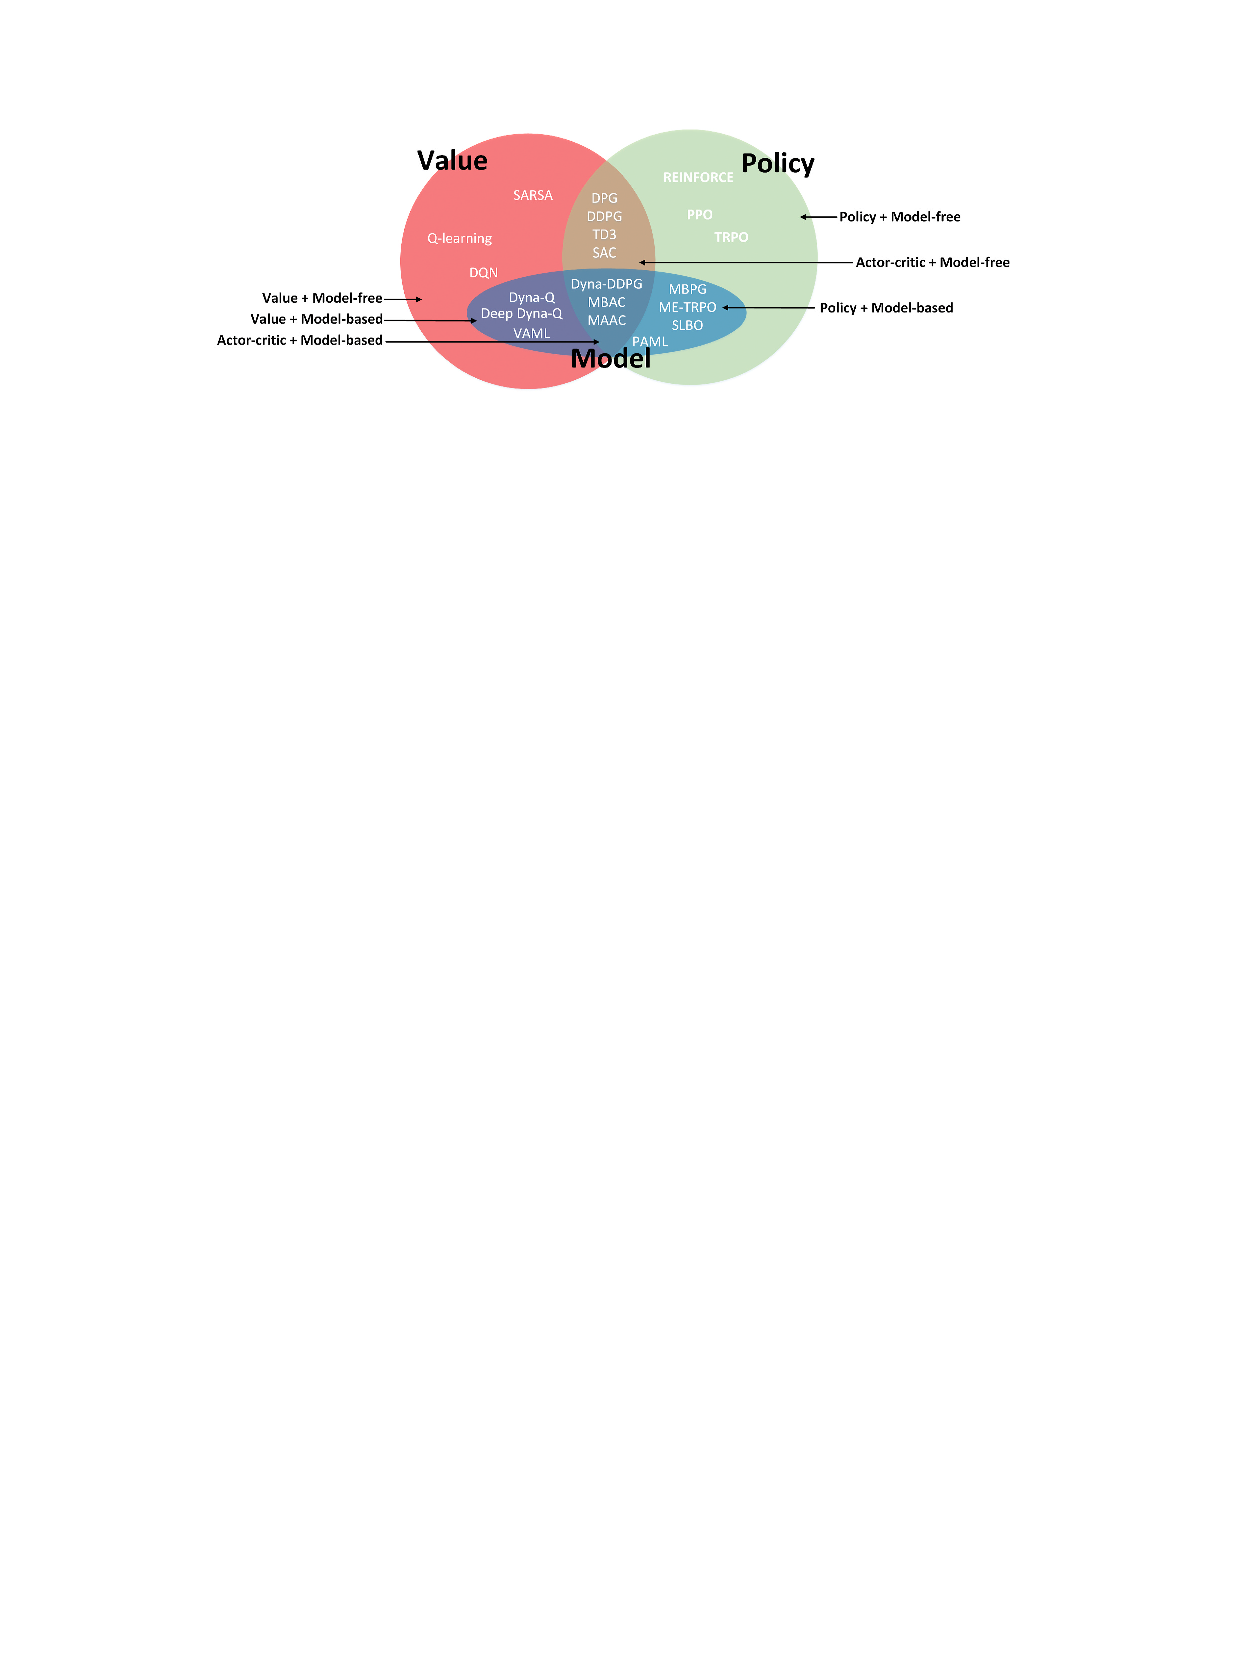
\includegraphics[width=\linewidth]{assets/2/rl_algorithm_taxonomy.pdf}
    \caption[Tassonomia dei principali algoritmi di RL e DRL moderni]{Tassonomia  dei principali algoritmi di RL e DRL moderni. Fonte: \cite{Perera2021}}
    \label{fig:2_rl_algorithm_taxonomy}
\end{figure}

\subsubsection{Metodi policy-gradient}

In DRL una policy viene rappresentata come una rete neurale con dei parametri $\theta$. Ogni insieme di valori $\theta$ rappresenta una particolare policy e l'addestramento dell'agente consiste nel trovare un insieme di valori $\theta$ che produce una policy ottimale.

I metodi policy-gradient hanno l'obiettivo di ottimizzare le prestazioni dell'agente trovando una policy $\pi_\theta$ in grado di generare una traiettoria $\tau$ che massimizza la ricompensa attesa, invece di apprendere una funzione di valore.

La funzione obiettivo nei metodi policy-gradient consiste nel massimizzare $J(\theta)$, ossia il valore atteso scontato per ottenere una policy $\pi_\theta$ aggiornando i parametri $\theta$:

\begin{equation}
    J(\pi_\theta) = \mathbb{E}_{\tau \sim \pi_\theta} \left[ \sum_{t=0}^{T} \gamma^t r_t\right],
\end{equation}

\begin{equation}
    \theta^\ast = \underset{\theta}{\arg\max} \, J(\pi_\theta).
\end{equation}

Si utilizza l'ascesa del gradiente stocastica per aggiornare i parametri $\theta$ in direzione positiva del gradiente della misura di prestazioni della policy $\nabla_\theta J(\theta)$, tramite la seguente equazione

\begin{equation}
    \theta \gets \theta + \alpha \nabla_\theta J(\pi_\theta),
\end{equation}

in cui $\alpha$ è uno scalare che regola il tasso di apprendimento.

Il vantaggio principale degli approcci policy-gradient risiede nella stabilità della loro convergenza: questi metodi funzionano aggiornando direttamente la loro policy a ogni passo, invece di aggiornare la funzione di valore da cui derivare la policy come nei metodi value-based. Quest'ultimi possono portare a un cambio radicale nell'output della policy anche per un piccolo cambio nella funzione di valore, causando oscillazioni prominenti durante l’addestramento. Inoltre, gli algoritmi policy-gradient possono affrontare spazi di azione continui poiché l’agente stima direttamente l’azione invece di calcolare il valore per ogni azione discreta possibile. La terza caratteristica è la loro capacità di apprendere policy stocastiche, utili in contesti incerti o ambienti parzialmente osservabili. Nonostante i vantaggi sopra menzionati, i metodi policy-gradient hanno uno svantaggio sostanziale: tendono a convergere verso un massimo locale invece che il massimo globale.

\paragraph{Architettura Actor-Critic.} Risulta naturale combinare due o più funzioni fondamentali, introdotte nella \Cref{sec:2_rl_algorithms_types}, per realizzare algoritmi che ottengano il meglio di ognuno. Un insieme di questi algoritmi sono quelli che imparano una policy e una funzione di valore, chiamati ``Actor-Critic''. Sono chiamati in questo modo perché la policy agisce, mentre la funzione di valore critica.

In DRL, ci sono due reti neurali: una che decide l'azione da intraprendere, chiamata ``Actor'', e una che valuta le azioni compiute dalla rete Actor, chiamata ``Critic''. Quest'ultima rete viene utilizzata per calcolare l'errore di previsione del valore, che è la differenza tra il valore stimato e il guadagno atteso, poi usato per aggiornare le due reti neurali.

L'idea alla base è che durante l'addestramento la funzione di valore può fornire più informazioni per la policy rispetto alla sequenza di ricompense date dall'interazione con l'ambiente. La policy impara a utilizzare le informazioni fornite dalla funzione di valore e le usa per generare azioni. L'algoritmo presentato e utilizzato nel seguente studio è di questa tipologia.

\subsection{Proximal Policy Optimization}
\label{sec:2_ppo}

Proximal Policy Optimization (PPO), introdotto in \cite{Schulman2017}, è un algoritmo di DRL di tipo policy-gradient, model-free che alterna il campionamento dei dati, tramite l'interazione con l'ambiente, con l'ottimizzazione di una funzione obiettivo surrogata utilizzando l'ascesa del gradiente stocastica. Ha una struttura Actor-Critic, pertanto impara la policy ottimale tramite la rete actor, e la funzione di valore tramite la rete critic, per cui è value-based. Inoltre PPO è policy-based poiché la rete actor impara la policy tramite metodi policy-gradient.

Un problema presente negli algoritmi policy-gradient è che sono suscettibili al collasso delle prestazioni, in cui un agente comincia ad agire male. Questo scenario è difficile da recuperare, poiché l'agente comincia a generare traiettorie poco utili per addestrare la policy. Inoltre un problema presente negli algoritmi on-policy è che non possono riutilizzare l'esperienza raccolta. PPO affronta questi due problemi introducendo una funzione obiettivo surrogata, la quale evita il collasso delle prestazioni garantendo dei miglioramenti monotonici per la policy. Tale obiettivo inoltre permette di riusare esperienza off-policy per la fase di addestramento.

\paragraph{Versioni di PPO.} PPO basa la sua ottimizzazione sul concetto di trust-region, ovvero l’introduzione di un vincolo tra gli aggiornamenti della policy, al fine di non avere cambiamenti troppo bruschi nell'aggiornamento della policy. Per fare ciò, PPO utilizza due euristiche: la prima basata sull'uso della penalità adattiva KL, la seconda basata sull'obiettivo surrogato clipped. Le due euristiche sono semplici da implementare ed efficaci; nell'articolo originale la versione con l'obiettivo surrogato clipped ha ottenuto prestazioni migliori rispetto all'altra, tuttavia le implementazioni disponibili in librerie pubblicamente accessibili forniscono abitualmente entrambe.

\subsubsection{Vantaggio} Nel contesto del RL e in particolare nei metodi basati su policy-gradient come PPO gioca un ruolo importante il concetto di vantaggio. Denotato con $A_t$, il vantaggio è una misura che quantifica quanto meglio, o peggio, sia eseguire una certa azione $a_t$ in uno stato $s_t$ rispetto al valore medio delle azioni in quello stato secondo la policy corrente. Può essere espresso come

\begin{equation}
    A_t = Q_t(s_t, a_t) - V_t(s_t)
\end{equation}

in cui $Q_t$ è la funzione azione-valore, rappresentante il guadagno atteso per l'azione $a_t$ dallo stato $s_t$, e $V_t$ è la funzione di valore, rappresentante il guadagno atteso medio dallo stato $s_t$, entrambe in base alla policy attuale $\pi$.

In PPO, il vantaggio è utilizzato per ponderare gli aggiornamenti della policy durante il processo di apprendimento. Se un’azione ha prodotto un vantaggio positivo significa che ha prodotto un guadagno superiore alla media e, di conseguenza, la probabilità di scegliere tale azione in futuro dovrebbe essere incrementata. Al contrario, se il vantaggio è negativo la probabilità di scegliere tale azione dovrebbe essere ridotta.

\subsubsection{Funzione obiettivo surrogata} PPO usa il concetto di massimizzazione della funzione obiettivo surrogata:

\begin{align}
    L^{\textnormal{CPI}}(\theta) &\coloneqq \mathbb{E}_t \left[ \frac{\pi_\theta(a_t | s_t)}{{\pi_\theta}_\textnormal{old}(a_t | s_t)} {A_t}^{{\pi_\theta}_\textnormal{old}} \right] \label{eq:2_ppo_surrogate_objective_full} \\
    &\coloneqq \mathbb{E}_t \left[ r_t(\theta) A_t \right], \label{eq:2_ppo_surrogate_objective}
\end{align}

in cui $\frac{\pi_\theta(a_t | s_t)}{{\pi_\theta}_\textnormal{old}(a_t | s_t)}$ rappresenta una stima della divergenza tra le due policy successive ${\pi_\theta}$ e ${\pi_\theta}_\textnormal{old}$, mentre ${A_t}^{{\pi_\theta}_\textnormal{old}}$ è il vantaggio calcolato con la vecchia policy.

Per semplicità di notazione si userà l'\Cref{eq:2_ppo_surrogate_objective}, che è equivalente all'\Cref{eq:2_ppo_surrogate_objective_full} con la differenza che $r_t(\theta) = \frac{\pi_\theta(a_t | s_t)}{{\pi_\theta}_\textnormal{old}(a_t | s_t)}$ e $A_t = {A_t}^{{\pi_\theta}_\textnormal{old}}$.

L'obiettivo è quello di valutare e migliorare la prestazioni della nuova policy $\pi_\theta$ rispetto alla vecchia ${\pi_\theta}_\textnormal{old}$. $L^{\textnormal{CPI}}(\theta)$ come funzione obiettivo è stata proposta inizialmente in \cite{Kakade2002}.

\subsubsection{Funzione obiettivo surrogata clipped}
\label{sec:2_ppo_funzione_obiettivo_clipped}

Senza un vincolo, la massimizzazione di $L^{\textnormal{CPI}}$ produrrebbe degli aggiornamenti alla policy troppo ampi che porterebbero a un collasso delle prestazioni. Per questo motivo $L^{\textnormal{CPI}}$ viene modificata penalizzando i cambiamenti di policy che rendono $r_t(\theta)$ eccessivamente lontano da 1:

\begin{equation}
    L^{\textnormal{CLIP}}(\theta) \coloneqq \mathbb{E}_t \left[ \min \left (r_t(\theta) A_t, \textnormal{clip}(r_t(\theta), 1 - \epsilon, 1 + \epsilon) A_t \right ) \right].
\end{equation}

$L^{\textnormal{CLIP}}$ è la funzione obiettivo surrogata clipped, in cui $\epsilon$ è un iperparametro che determina il grado di variazione ammesso per la policy in ogni aggiornamento, per evitare aggiornamento troppo bruschi che potrebbero destabilizzare l'apprendimento.

Notare che il primo termine di $\min$ è $L^{\textnormal{CPI}}$. Il termine $\textnormal{clip}(r_t(\theta), 1 - \epsilon, 1 + \epsilon)$ rimuove l'incentivo di muovere $r_t$ al di fuori dell'intervallo $[1 - \epsilon, 1 + \epsilon]$.

La funzione $L^{\textnormal{CLIP}}$ calcola quindi il valore minimo tra i due termini indicati, allo scopo di impedire variazioni troppo significative della policy, proteggendo il processo di apprendimento da possibili instabilità e oscillazioni.

La \Cref{fig:2_ppo_clip} mostra il funzionamento di $L^{\textnormal{CLIP}}$ in un singolo passo $t$.

\begin{figure}
    \centering
    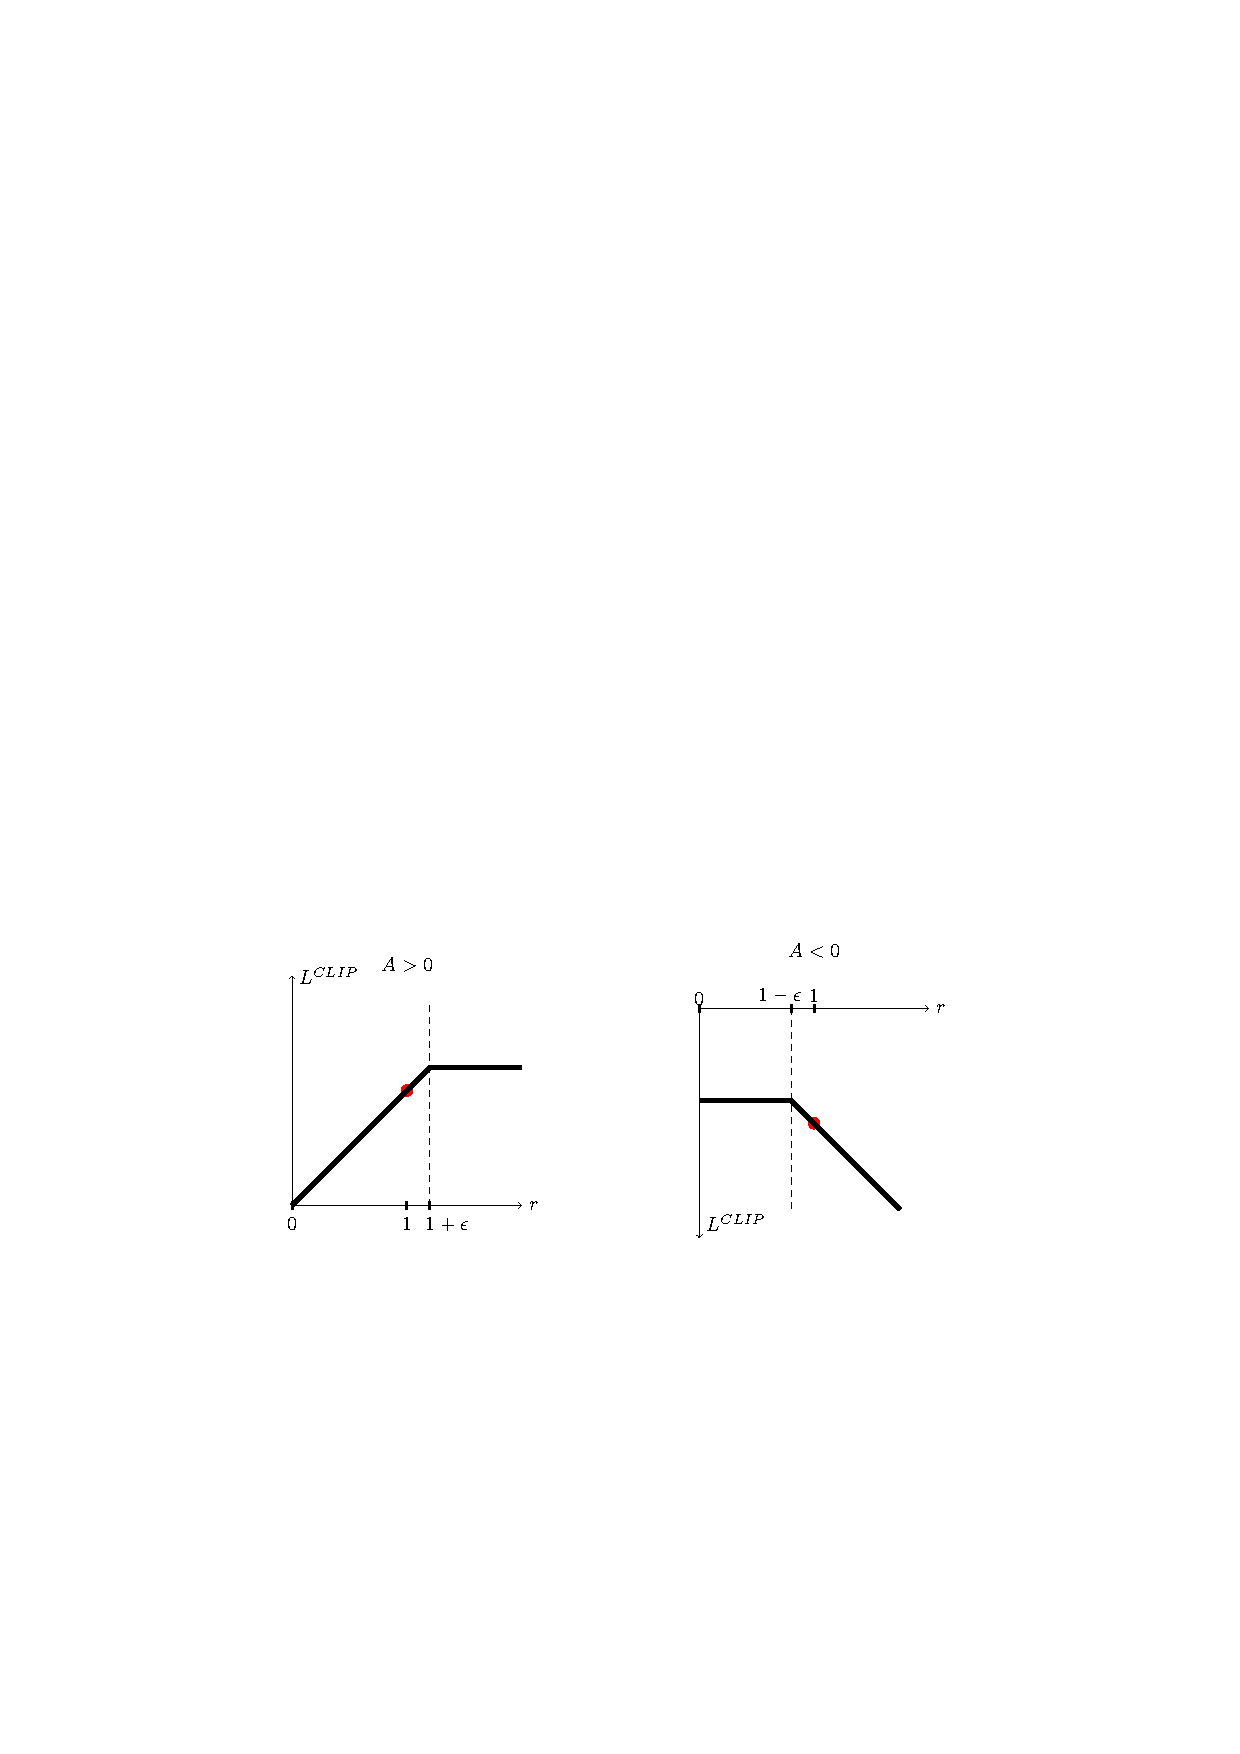
\includegraphics[width=.7\linewidth]{assets/2/ppo_clip.pdf}
    \caption[Esempio di funzionamento di $L^{\textnormal{CLIP}}(\theta)$]{Esempio di funzionamento di $L^{\textnormal{CLIP}}(\theta)$ come funzione del rapporto di probabilità $r$. A sinistra il caso di un vantaggio positivo, a destra un vantaggio negativo. In rosso è rappresentato il punto iniziale di ottimizzazione (in questo esempio $r = 1$. Fonte: \cite{Schulman2017}}
    \label{fig:2_ppo_clip}
\end{figure}
    
\subsubsection{Penaltà KL adattiva}

Un'alternativa alla funzione obiettivo surrogata clipped, applicabile separatamente oppure in aggiunta, è di utilizzare una penalità basata sulla divergenza di Kullback–Leibler\footnote{Una misura non simmetrica della differenza tra due distribuzioni di probabilità.} (KL), e di adattare un coefficiente di penalità in base al problema. $L^{\textnormal{CPI}}$ viene quindi modificata nel modo seguente:

\begin{equation}
    L^{\textnormal{KLPEN}}(\theta) \coloneqq \mathbb{E}_t \left[ r_t(\theta) A_t - \beta \, \textnormal{KL}[{\pi_\theta}_\textnormal{old}(\cdot | s_t), \pi_\theta(\cdot, s_t)] \right].
\end{equation}

$L^{\textnormal{KLPEN}}$ è la funzione obiettivo surrogata KL-penalizzata, in cui $\beta$ è un coefficiente adattivo che controlla la dimensione della penalità KL. $\beta$ è aggiornato a ogni aggiornamento della policy e il nuovo valore viene utilizzato nella successiva iterazione. L'aggiornamento si basa sulla comparazione di un iperparametro $d_\textnormal{targ}$ e dal valore $d = \mathbb{E}_t \left[ \textnormal{KL}[{\pi_\theta}_\textnormal{old}(\cdot | s_t), \pi_\theta(\cdot, s_t)] \right]$:

\begin{itemize}
    \item Se $d < d_\textnormal{targ} / 1.5$, allora $\beta \gets \beta / 2$,
    \item Se $d > d_\textnormal{targ} \times 1.5$, allora $\beta \gets \beta \times 2$.
\end{itemize}

Il valore iniziale dell'iperparametro $\beta$ non è rilevante perché l'algoritmo lo corregge automaticamente, mentre i parametri costanti $1.5$ e $2$ sono state scelte euristicamente in \cite{Schulman2017}, ma l'algoritmo non è particolarmente sensibile a tali valori.

\subsubsection{L'algoritmo}

Come già introdotto, PPO adotta un'architettura Actor-Critic. Questa architettura permette di formulare una funzione obiettivo che integra l'ottimizzazione delle due reti neurali, incorporando sia la differenza tra i valori previsti dalla rete Critic e il guadagno effettivo, sia la differenza tra le azioni scelte dalla rete Actor e quelle ottimali.

Inoltre si aggiunge un bonus di entropia $S$, che serve a incoraggiare una maggiore esplorazione da parte della rete Actor, prevenendo la convergenza prematura verso una policy deterministica. La funzione obiettivo risultante, in base alla scelta di usare $L^{\textnormal{CLIP}}$ o $L^{\textnormal{KLPEN}}$ (o entrambi), massimizzata a ogni iterazione è la seguente:

\begin{equation}
    L^{\textnormal{CLIP+VF+S}}_t(\theta) \coloneqq \mathbb{E}_t \left[ L^{\textnormal{CLIP}}_t(\theta) - c_1 L^{\textnormal{VF}}_t + c_2 S[\pi_\theta](s_t) \right]
\end{equation}

in cui $c_1$ e $c_2$ sono dei coefficienti, $S$ è il bonus di entropia e $L^{\textnormal{VF}}_t$ è l'errore quadratico $(V_\theta(s_t) - V^{\textnormal{targ}}_t)^2$.

PPO esegue la policy per un numero di passi $T$, un numero minore della lunghezza totale dell'episodio, in modo da ottenere più minibatch (insieme di esperienza) da ogni episodio. Ciò consente di realizzare aggiornamenti frequenti e informativi della policy, senza necessità di completare interi episodi.

L'algoritmo è mostrato in \Cref{alg:2_ppo} come pseudocodice. Nella sua versione originale, sono presenti $N$ attori che eseguono contemporenamente la policy ${\pi_\theta}_\textnormal{old}$ in diversi ambienti per $T$ passi, raccogliendo l'esperienza raccolta come forma di traiettorie. L'ottimizzazione viene effettuata con l'esperienza raccolta tramite SDG (discesa del gradiente stocastica) in minibatch, ognuno di dimensione $M$.

\begin{algorithm}
    \caption[Pseudocodice di Proximal Policy Optimization (PPO)]{Pseudocodice di Proximal Policy Optimization (PPO)}
    \label{alg:2_ppo}
    \begin{algorithmic}[1] % Every line gets a number.
        \For{iterazione = 1, 2, ...}
            \For{attore = 1, 2, ..., $N$}
                \State Esegui la policy ${\pi_\theta}_\textnormal{old}$ nell'ambiente per $T$ passi;
                \State Calcola le stime dei vantaggi $A_1, \dots, A_t$ usando ${\pi_\theta}_\textnormal{old}$;
            \EndFor
            \State Ottimizza $L(\theta)$, per $K$ epoche e con la dimensione dei minibatch $M \le NT$;
            \State $\theta_\textnormal{old} \gets \theta$;
        \EndFor
    \end{algorithmic}
\end{algorithm}

Il calcolo dei vantaggi è definito come

\begin{equation}\label{eq:2_ppo_advantages}
    A_t = \delta_t + (\gamma \lambda) \delta_{t+1} + \dots + (\gamma \lambda)^{T-t+1} \delta_{T-1},
\end{equation}

in cui $\delta_t = r_t + \gamma V(s_{t+1}) - V(s_t)$ e $t$ è un indice temporale in $[0, T]$. L'\Cref{eq:2_ppo_advantages} è una versione troncata della stima del vantaggio generalizzata (GAE), introdotta in \cite{Schulman2015}.

\subsection{Scelte per il caso di studio}
\label{sec:2_rl_ppo_choices}

Nella modellazione del problema DFaaS, approfondita nella \Cref{sec:4_environments}, è stato scelto uno spazio di azione continuo per indicare quali richieste sono da processare localmente, inoltrare e rifiutare. Questo ha condizionato la scelta dell'algoritmo, perché non tutti sono compatibili con tale spazio. PPO è un algoritmo che supporta gli spazi d'azione continui. Inoltre è facile da implementare e non richiede troppe risorse computazionali. Rispetto ad altri algoritmi simili come Soft Actor-Critic (SAC), ha dimostrato prestazioni migliori in problemi simili a quello affrontato \cite{Haarnoja2018, Petriglia2024}.

Nel considerare la modellazione multi-agente, sono stati sperimentati due approcci principali di MARL con PPO:

\begin{itemize}
    \item Fase di addestramento ed esecuzione decentralizzata: in cui ogni agente ha una policy indipendente dalle altre, imparata con le osservazioni locali dell'agente. In termini pratici, significa utilizzare PPO per ogni agente.

    \item Fase di addestramento centralizzata ed esecuzione decentralizzata: nella fase di addestramento PPO viene eseguiti in modo centralizzato condividendo i parametri della rete Critic per tutti gli agenti, mentre la rete Action, quella che apprende la policy, rimane indipendente. Nella fase di esecuzione ogni agente ottiene una copia della rete Critic addestrata ed esegue la policy senza la condivisione delle informazioni.
\end{itemize}

\chapter{Stato dell'arte}
\label{sec:3_stato_arte}

In questo capitolo sono riportati alcuni studi presenti nella letteratura scientifica relativi alla distribuzione del lavoro in ambienti edge ed edge-cloud, considerando sia approcci euristici \cite{Chai2021, Hsieh2023} sia basati sull'Apprendimento per Rinforzo \cite{Liu2023, Zhang2023}. In questo contesto, il machine learning e in particolare il RL hanno recentemente acquisito popolarità, per via della loro capacità di effettuare decisioni rapide sulla distribuzione del lavoro in ambienti dinamici e parzialmente osservabili \cite{Hortelano2023, Kar2023}.

\section{Survey su approcci basati su ML/RL}

In \cite{Kar2023} viene presentato un ampio sondaggio sui metodi di ottimizzazione proposti in letteratura per la distribuzione del lavoro in ambienti federati che utilizzano più paradigmi di computazione. Viene proposta una classificazione degli ambienti, in base ai paradigmi utilizzati e la tipologia di federazione (orizzontale o verticale). Vengono inoltre definiti i possibili metodi di distribuzione del lavoro (es. da edge a edge o da edge a cloud) e gli scenari, mostrati in \Cref{fig:2_task_offloading_scenarios}: il primo scenario (1) coinvolge dispositivi in una posizione localizzata con poca mobilità, il secondo (2) coinvolge i veicoli con grande mobilità, mentre il terzo (3) descrive il traffico generato dai dispositivi IoT industriali. Ogni scenario ha le sue caratteristiche e richieste in termini di latenza e qualità del servizio.

\begin{figure}
    \centering
    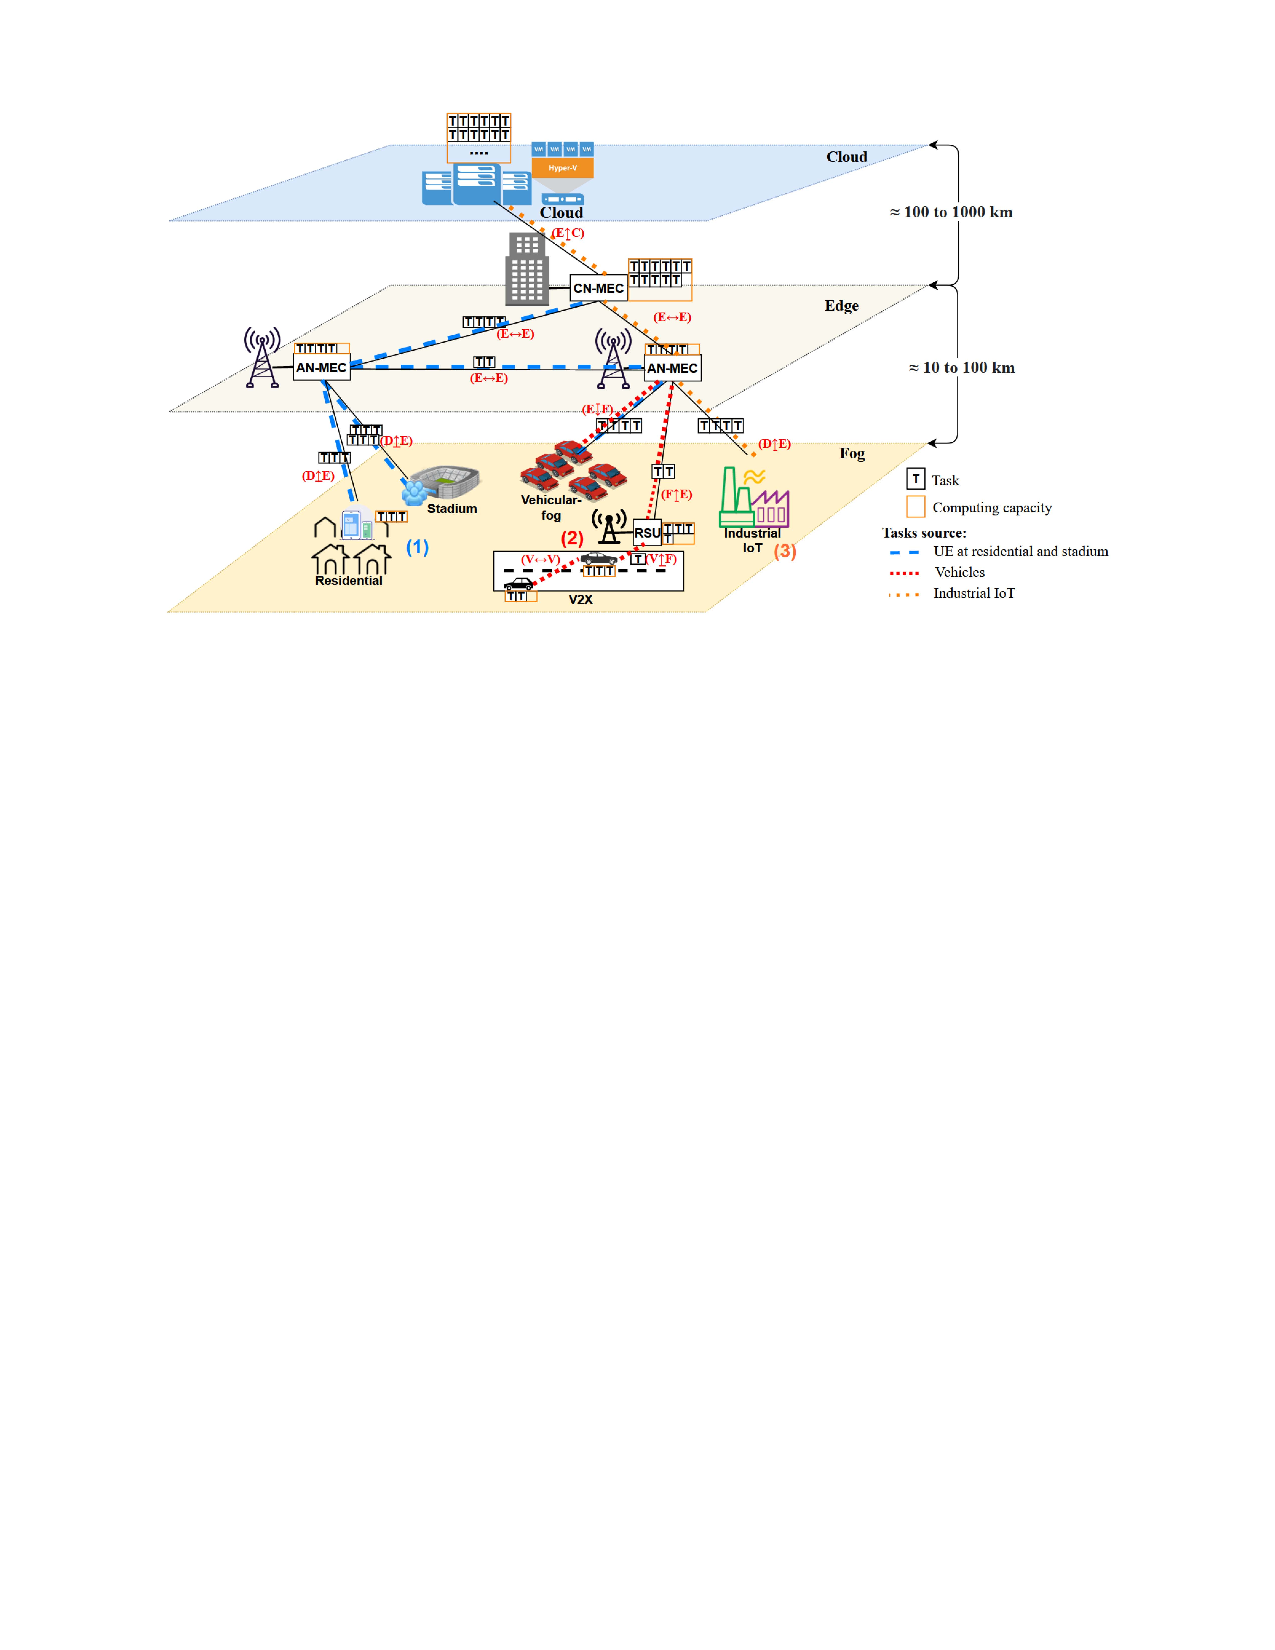
\includegraphics[width=\textwidth]{assets/3/task_offloading_scenarios.pdf}
    \caption[Distribuzione del lavoro nel cloud-edge-fog federato]{Distribuzione del lavoro nel cloud-edge-fog federato. Fonte: \cite{Kar2023}}
    \label{fig:2_task_offloading_scenarios}
\end{figure}

In base alla tipologia di ambiente e di scenario sono presentati una serie di approcci, partendo dai metodi di ottimizzazione tradizionali, che svolgono una ricerca spesso esaustiva per trovare una soluzione ottimale e richiedono una conoscenza esatta del sistema. Tra i lavori presentati, la maggior parte fanno uso di euristiche (metodo di bisezione, ottimizzazione iterativa a due fasi) oppure di algoritmi dinamici, valutati principalmente su ambienti simulati e che si concentrano sulla gestione del traffico. Metodi di questo tipo richiedono troppo tempo per convergere in scenari di larga scala e che devono garantire una latenza ridotta. Per questo approcci, di tipo ML hanno acquisito popolarità, in particolare il Deep Learning. Un limite dell'apprendimento supervisionato, tuttavia, è la necessità di richiedere un insieme di dati etichettato, non sempre possibile in ambienti così dinamici come può essere la rete, oltre a essere poco adattabile in nuovi scenari incontrati. Il RL, invece, ha ottime proprietà di adattamento poiché apprende tramite l'interazione diretta con l'ambiente. Tra i vari studi presentati che usano il RL e il Deep RL, la maggior parte adotta gli algoritmi DPPG\footnote{Deep Deterministic Policy Gradient.} e DQN\footnote{Deep Q-Network.}, entrambi di tipo off-policy e addestrati su ambienti simulati e per applicazioni relative ai tre scenari individuati. Tra tutti gli studi analizzati, un paio fa riferimento alla distribuzione del traffico tra nodi edge utilizzando metodi tradizionali, mentre nessuno con metodi ML. Inoltre nessuno studio si svolge in un contesto di FaaS.

Il survey di \cite{Hortelano2023} approfondisce maggiormente l'uso del RL, e in particolare del DRL, per la distribuzione del lavoro in ambienti di computazione edge. Vengono analizzati diversi lavori, suddivisi in base ad alcune caratteristiche, tra cui le metriche da massimizzare (o da minimizzare), l'architettura della rete di servizi e l'approccio scelto per la decisione sulla distribuzione del lavoro tra nodi. Quest'ultima categoria è mostrata in \Cref{fig:2_rl_decision_approaches} ed è costituita di tre approcci distinti: un singolo agente centralizzato, un sistema multi-agente posizionato sui nodi edge, oppure nei dispositivi finali.

\begin{figure}
    \centering
    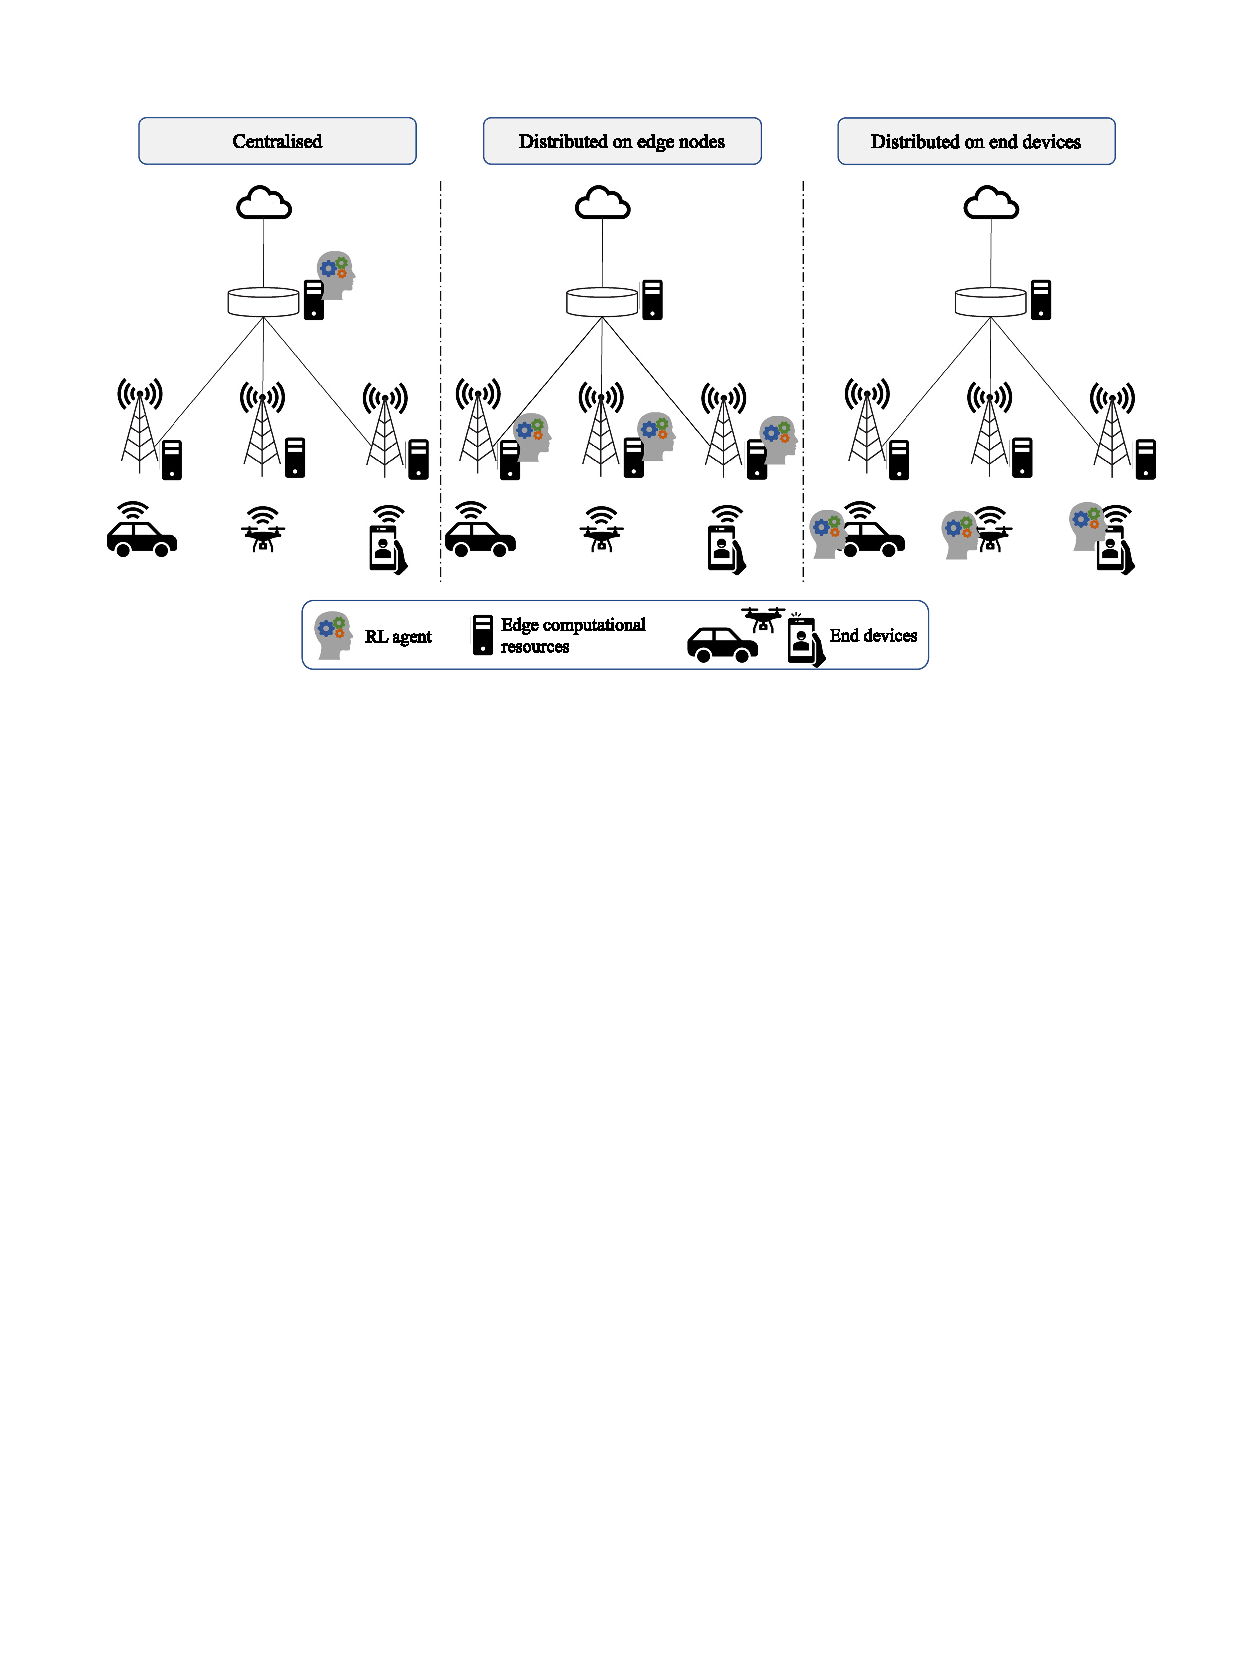
\includegraphics[width=\textwidth]{assets/3/rl_decision_approaches.pdf}
    \caption[Possibili posizionamenti degli agenti RL nella rete edge]{Possibili posizionamenti degli agenti RL nella rete edge. Fonte: \cite{Hortelano2023}}
    \label{fig:2_rl_decision_approaches}
\end{figure}

I lavori analizzati sono stati suddivisi in cinque casi di studio: reti IoT, reti veicolari, reti di UAV\footnote{Aeromobile a pilotaggio remoto (unmanned aerial vehicle), usati come punti di accesso mobili alla rete in caso di disastri naturali o emergenze.}, casi d'uso specifici come realtà virtuale o robotica e studi generici. La maggior parte dei lavori riguarda studi generici, senza focalizzarsi su una rete precisa. Gli algoritmi di RL più utilizzati sono DQN e DDQN, nell'ambito del Q-Learning e quindi value-based. Solo una minima parte dei lavori utilizza PPO. Le principali metriche ottimizzate sono la minimizzazione della latenza e del consumo di energia, solo al terzo posto si trova la massimizzazione dei lavori completati, che in un contesto FaaS può corrispondere al numero di richieste correttamente processate. L'approccio di nostro interesse, cioè distribuito sui nodi edge, risulta essere solo il terzo più comune tra quelli adottati nei lavori analizzati. Anche in questo sondaggio non è presente uno studio all'interno di un contesto di FaaS.

\section{Metodi euristici e RL su ambienti edge}

Tra la moltitudine di lavori incentrati sulla distribuzione del traffico in ambienti edge, abbiamo selezionato quattro lavori di interesse non presenti nei sondaggi citati nella sezione precedente.

In \cite{Chai2021} viene proposto uno schedulatore dinamico basato su priorità e un algoritmo di distribuzione per lavori di priorità diversa. In base alla priorità dei lavori vengono utilizzati approcci diversi: per quelli di alta priorità si impiega un algoritmo euristico basato sul problema dello zaino (knapsack problem), mentre un algoritmo basato sui pesi dei lavori\footnote{Pesi calcolati come la distanza di salti che di un lavoro al lavoro finale, all'interno di un grafo direzionale che rappresenta le dipendenze tra lavori.} e dimensione dei dati è usato per lavori di media priorità.

Sullo stessa tipologia di algoritmi euristici, in \cite{Hsieh2023} viene proposto l'algoritmo Knapsack Potential Game (KPG) per un meccanismo di distribuzione dall'edge al cloud per garantire il servizio per il traffico di alta e bassa priorità. In uno scenario di reti mobili 5G, usando KPG si ottiene un rapporto ottimale di distribuzione per ogni nodo edge che bilancia il costo-efficacia dell'intero sistema, con una bassa complessità computazionale e prestazioni migliori rispetto a due algoritmi base usati come riferimento, uno di tipo greedy e l'altro di tipo cooperativo.

Per metodi strettamente di RL, \cite{Liu2023} si concentra nella minimizzazione del \textit{deadline violation ratio} (DVR), definito come la percentuale di applicazioni non terminate in un orizzonte temporale finito, considerando il carico in ingresso e i ritardi in un contesto di \textit{mobile edge computing} (MEC) in cui la computazione viene portata al bordo della rete cellulare. Viene utilizzato un algoritmo basato su DDPG per determinare la policy ottimale di distribuzione per applicazioni mobile con lavori interconnessi da una rete di dipendenze, ottenendo una riduzione del DVR del 60-70\% rispetto a benchmark esistenti su vari scenari di rete.

Infine in \cite{Zhang2023} viene affrontato il problema per lo stesso contesto MEC 5G, proponendo un algoritmo multi-obiettivo di RL (Multi-Objective Reinforcement Learning, MORL) basato su DDQN per approssimare dinamicamente la decisione ottimale nel contesto di Internet dei veicoli (Internet of vehicles, IoV). MORL generalizza il metodo tradizionale di RL, poiché la ricompensa da un singolo scalare diventa un vettore di scalari. L'agente nell'approccio MORL impara a ottimizzare due o più obiettivi simultaneamente, i quali possono essere correlati positivamente o negativamente (conflittuali) oppure non correlati. MORL può essere pertanto visto come la combinazione dell'ottimizzazione multi-obiettivo con il RL.

L'agente ottiene dall'ambiente definito in \cite{Zhang2023} feedback multipli calcolati in base a parametri di ritardo, energia consumata, carico computazionale ed entropia di riservatezza\footnote{Misura della sicurezza dei dati trasmessi.}. La \Cref{fig:2_morl_vs_rl} mostra la differenza tra MORL e RL tradizionale; notare che l'approccio multi-agente (MARL) è ortogonale a MORL, poiché MARL è caratterizzato dalla presenza di più agenti.

\begin{figure}
    \centering
    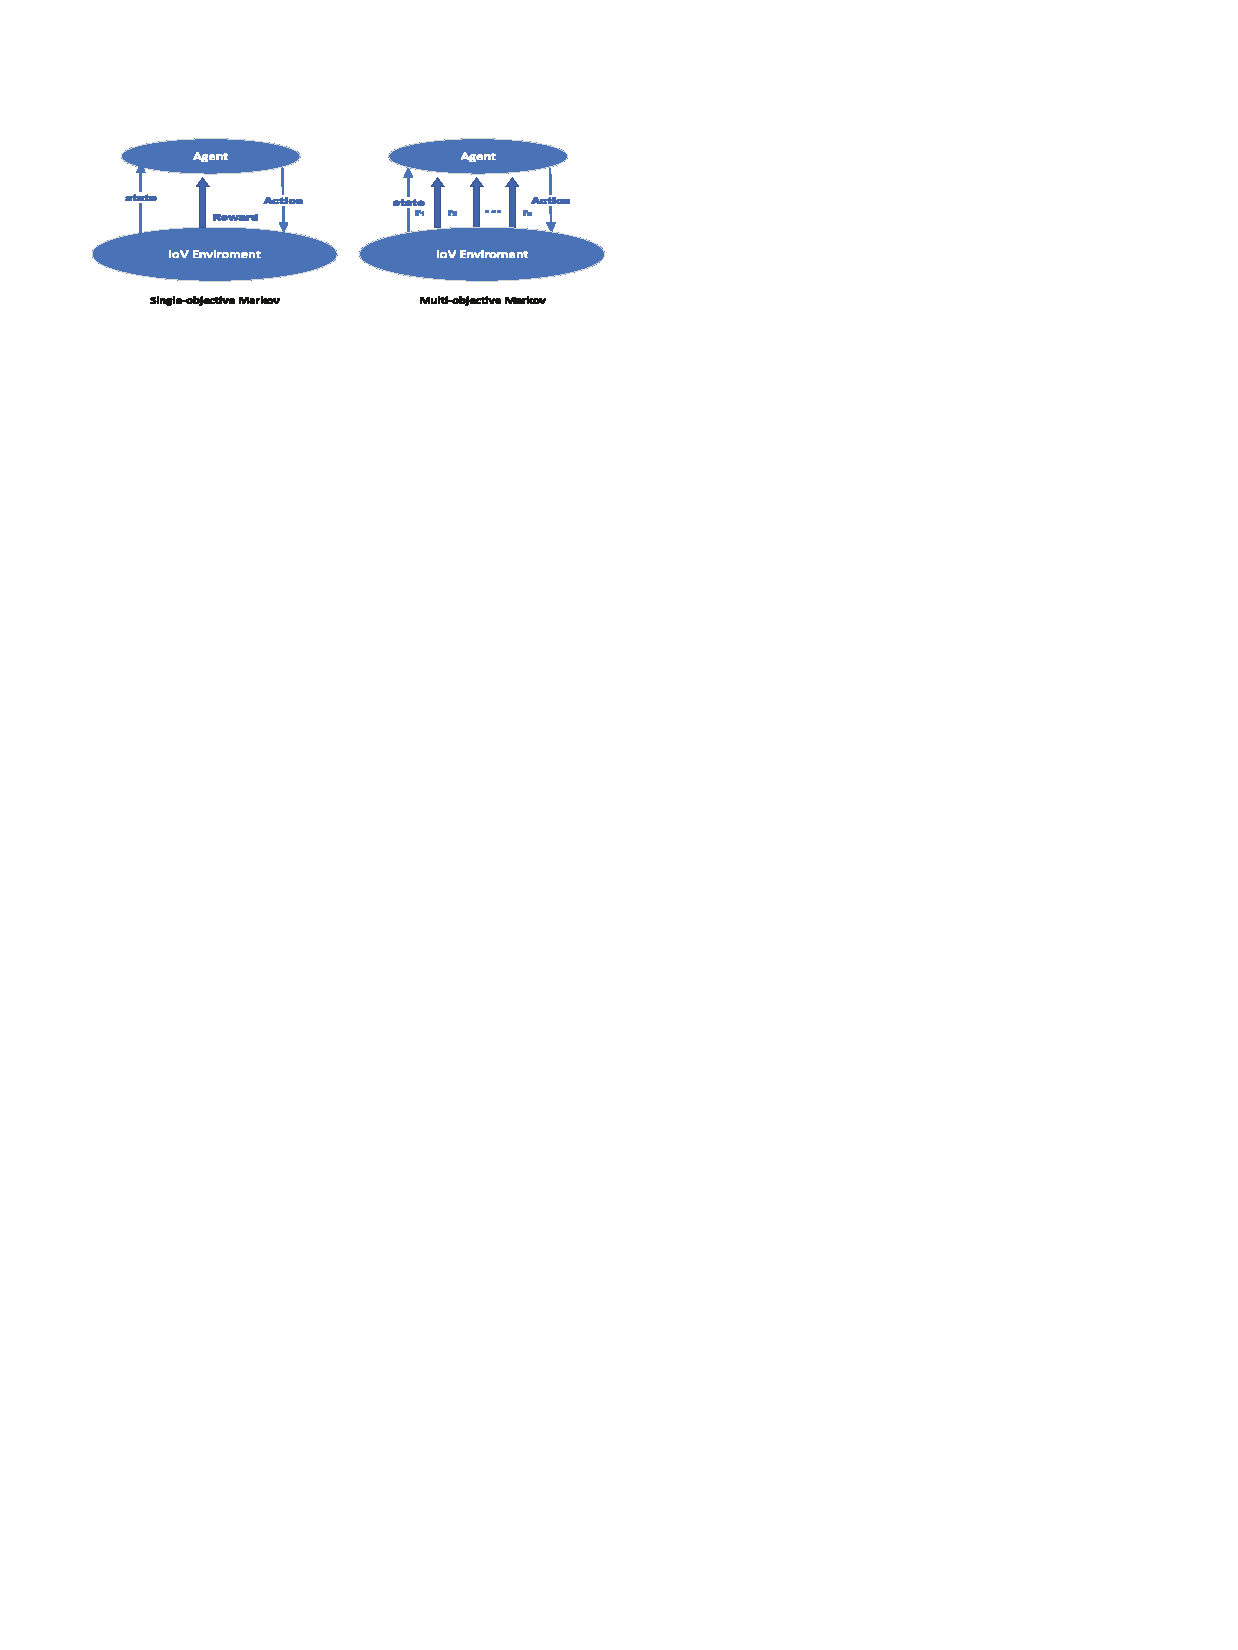
\includegraphics[width=.8\linewidth]{assets/3/morl_vs_rl.pdf}
    \caption[Differenza tra RL tradizionale e RL multi-obiettivo]{Differenza tra RL tradizionale e RL multi-obiettivo. Fonte: \cite{Zhang2023}}
    \label{fig:2_morl_vs_rl}
\end{figure}

\section{Apprendimento per Rinforzo su ambienti FaaS}

Nonostante tutti i lavori menzionati mostrino risultati promettenti utilizzando metodi di RL per affrontare il problema della distribuzione del traffico, nessuno di questi tratta nello specifico sistemi FaaS in ambienti edge, contesto principale di questa tesi.

Considerando unicamente l'ambiente FaaS, \cite{Fuerst2022} propone un algoritmo di bilanciamento del carico progettato per applicazioni FaaS, con l'obiettivo di bilanciare la località, la distribuzione del carico e l'imprevedibilità. I problemi principali con algoritmi di bilanciamento del carico classici è che non considerano le caratteristiche uniche delle funzioni di sistemi FaaS: l'inizializzazione delle funzioni richiede tempo ed è tipicamente omogenea per tutte le tipologie di funzioni, mentre il carico di lavoro è eterogeneo: solo una piccola frazione delle funzioni viene invocata per la maggior parte delle invocazioni. Per questo motivo gli autori utilizzano un sistema di hash coerente\footnote{Tecnica di hash in cui al ridimensionamento della tabella di hash solo una porzione delle chiavi richiede di essere rimappata.} per preservare la località in caso di aggiunta o rimozione di nodi FaaS, fondamentale per gestire i picchi di carico. Sebbene sia simile al lavoro di questa tesi nella gestione di applicazioni serverless, \cite{Fuerst2022} si focalizza su server generici e non considera gli aspetti specifici posti dagli ambienti edge.

In \cite{Petriglia2024}, il lavoro precedente a questa tesi, vengono comparati due algoritmi di RL, PPO e SAC\footnote{Soft Actor-Critic, un algoritmo off-policy con la stessa architettura Actor-Critic di PPO.}, e l'algoritmo generico NEAT\footnote{NeuroEvolution of Augmenting Topologies, che si basa sulla generazione evolutiva di reti neurali.} addestrando un singolo agente in un ambiente che modella la distribuzione del carico in un sistema di computazione edge-FaaS. Il sistema modellato è raffigurato in \Cref{fig:2_single_agent_env} e coinvolge un nodo in grado di processare le richieste localmente, inoltrarle ai nodi vicini e rifiutarle. Gli algoritmi sono stati provati su tre tipologie di carico. L'agente, nel sistema proposto, osserva la disponibilità di inoltro e il carico in ingresso al passo successivo. PPO è risultato l'algoritmo migliore rispetto a SAC e NEAT in termini di richieste rifiutate per episodio.

Il lavoro di questa tesi è un diretto proseguimento di \cite{Petriglia2024}: si supera l'ambiente a singolo agente introducendo un ambiente multi-agente (descritto nel \Cref{sec:4_modellazione}), per addestrare gli agenti viene utilizzato PPO in due configurazioni MARL, le tre tipologie di carico di prova sono riproposte, tuttavia una di questa viene sostituita con dati reali e non generati (descritta nella \Cref{sec:5_scenario_reale}).

\begin{figure}
    \centering
    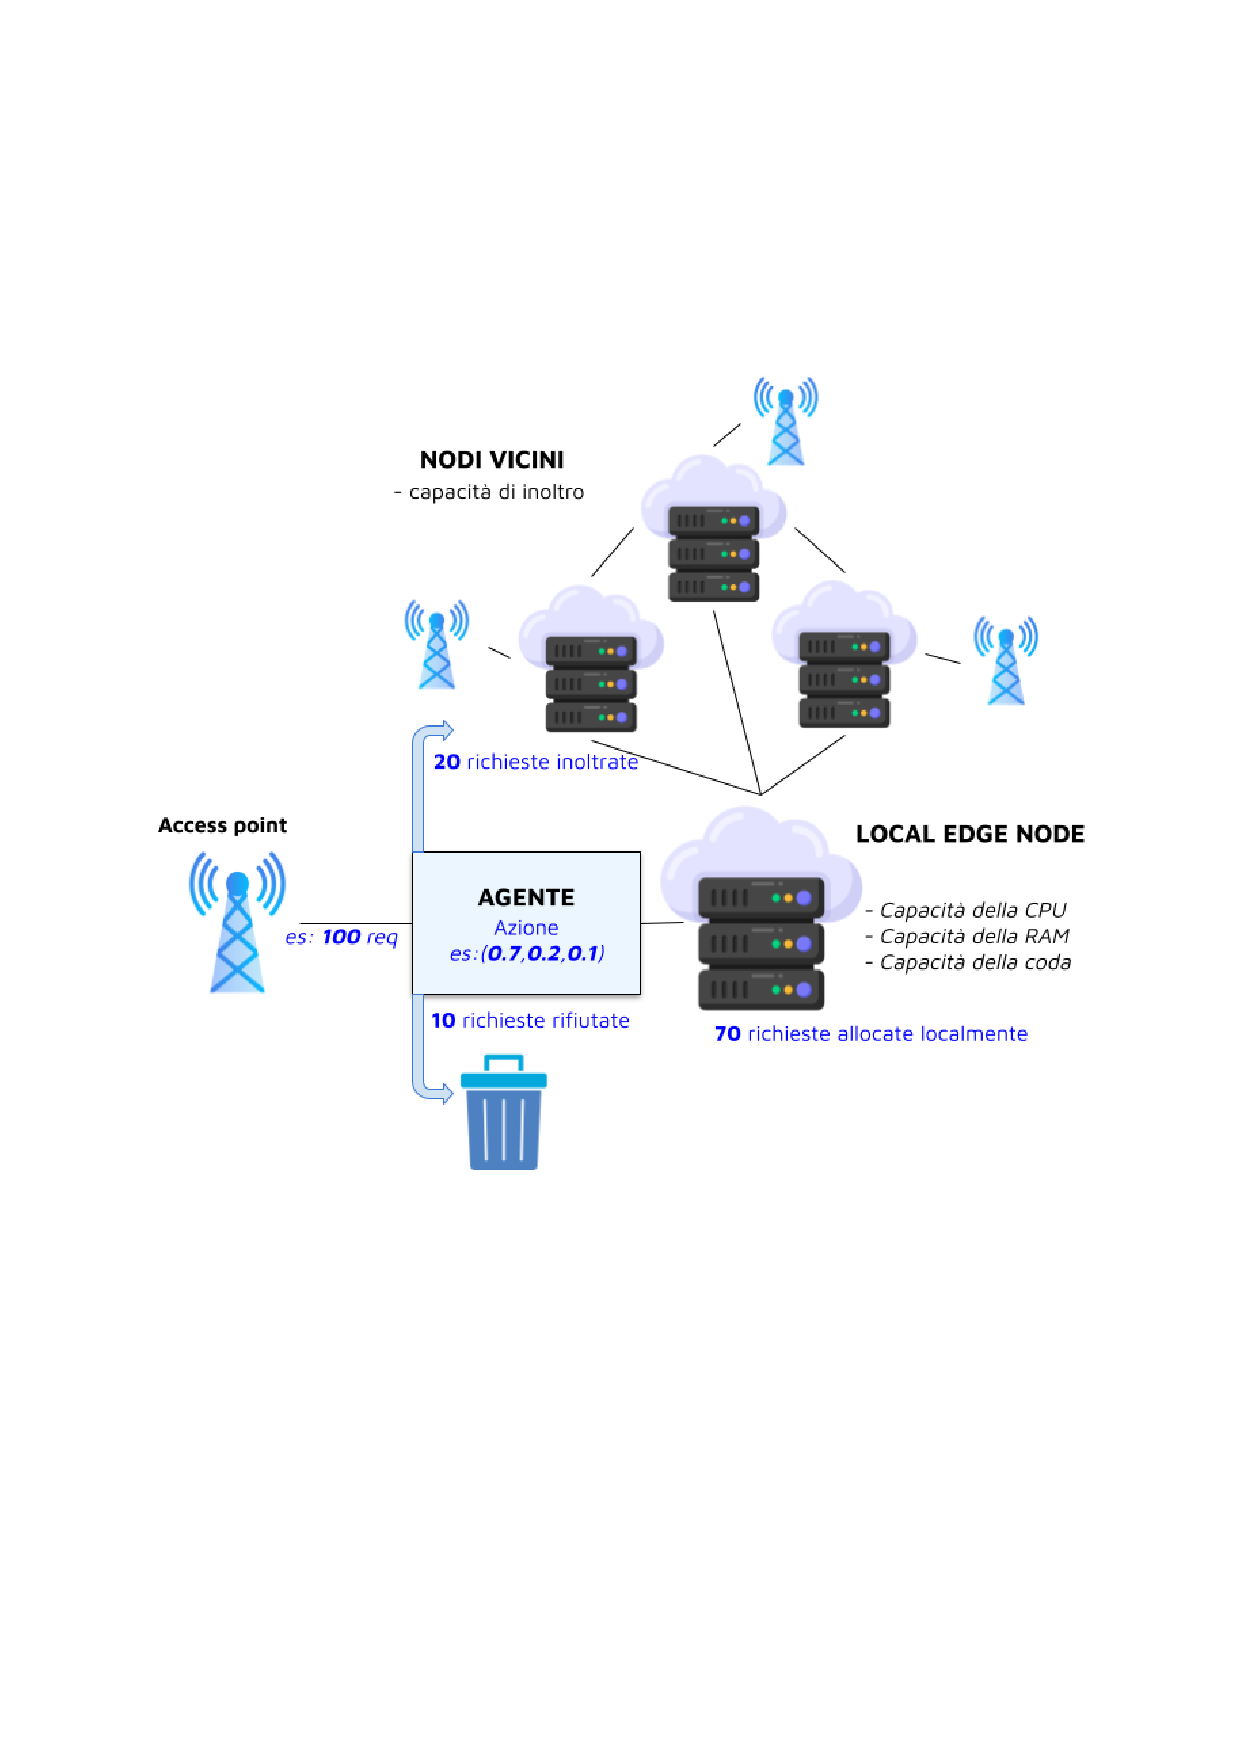
\includegraphics[width=.8\linewidth]{assets/3/single_agent_env.pdf}
    \caption[Sistema modellato a singolo agente.]{Sistema modellato a singolo agente. L'agente decide come distribuire le richieste attraverso una distribuzione, nell'esempio $(0.7, 0.2, 0.1)$, che viene poi convertita nel numero di richieste da distribuire $(70, 20, 10)$. Fonte: \cite{Petriglia2024}}
    \label{fig:2_single_agent_env}
\end{figure}

\chapter{Modellazione degli ambienti}
\label{sec:4_modellazione}

In questo capitolo viene descritta la modellazione degli ambienti proposti per la distribuzione del carico all'interno di un sistema edge-FaaS. Sono stati modellati tre ambienti multi-agente, di complessità incrementale, insieme alle dinamiche in cui le policy operano. Diverse ipotesi semplificatrici sono state introdotte rispetto allo scenario reale per investigare se il Reinforcement Learning può essere una valida soluzione per la distribuzione del carico, con l'obiettivo finale di progettare un ambiente reale multi-agente adatto per la piattaforma DFaaS.

Come introdotto nella \Cref{sec:2_mdp}, un ambiente MARL è caratterizzato da uno spazio delle osservazioni e delle azioni per ogni agente, una funzione di ricompensa per agente e uno stato interno (globale o locale) dell'ambiente che contiene informazioni sul sistema simulato.

Nelle seguenti sezioni sono dettagliate le singole proprietà degli ambienti modellati.

\section{Elementi del sistema}
\label{sec:4_modellazione_elementi}

Data la moltitudine di elementi che compongono il problema affrontato, in questa sezione sono raccolti in un unico posto tutte le variabili che definiscono l'ambiente con una definizione concisa.

Due insiemi importanti sono l'insieme degli agenti $\mathcal{N}$ e l'insieme dei passi $T$, entrambi finiti in $\mathbb{N}^0$. Ogni variabile fa riferimento a un agente $n \in \mathcal{N}$ al $t$-esimo passo\footnote{Gli indici dell'agente o del passo sono omessi a meno di ambiguità.} ($t \in T$):

\begin{itemize}
    \item Richieste in input $R^\textnormal{IN}$: rappresenta il numero di richieste in ingresso che l'agente che deve distribuire.

    \item Capacità della coda $q^\textnormal{MAX}$: rappresenta il numero di slot disponibili che si possono utilizzare per processare localmente le richieste.

    \item Capacità residua della coda $q^\textnormal{FREE}$: rappresenta il numero di slot disponibili a seguito dell'allocazione delle richieste da processare localmente.

    \item Capacità di inoltro $F$: rappresenta il numero di richieste che un agente può inoltrare ad altri agenti.

    \item Eccesso di processamento locale $e^\textnormal{L}$: rappresenta il numero di richieste che l'agente ha tentato di processare localmente ma che eccedono la capacità della coda, e che pertanto sono considerate rifiutate.

    \item Eccesso di rifiuto $e^\textnormal{R}$: rappresenta il numero di richieste rifiutate che potevano essere processate localmente oppure inoltrate senza essere rifiutate.

    \item Eccesso di inoltro $e^\textnormal{FW}$: rappresenta il numero di richieste inoltrate in eccesso, cioè richieste che sono state inoltrate ma che potevano essere processate localmente.

    \item Richieste inoltrate ma rifiutate $e^\textnormal{FR}$: rappresenta il numero di richieste inoltrate da un agente che sono state rifiutate dagli altri agenti. È anche indicato come $s^\textnormal{FR}$ se la variabile fa riferimento all'osservazione.
\end{itemize}

\section{Definizione degli ambienti}
\label{sec:4_environments}

I tre ambienti modellati differiscono per la capacità degli agenti di inoltrare o meno le richieste in ingresso agli altri agenti. Di complessità incrementale, ad alto livello sono così definiti:

\begin{itemize}
    \item \textbf{Ambiente simmetrico senza inoltro}: gli agenti sono completamente indipendenti l'uno dall'altro e possono soltanto processare localmente o rifiutare le richieste in arrivo. Etichettato come ``BASE'' di seguito.

    \item \textbf{Ambiente asimmetrico}: gli agenti sono divisi in due gruppi disgiunti, uno in grado di inoltrare le richieste agli altri nodi e uno che può soltanto processare le richieste localmente o rifiutarle. Etichettato come ``ASYM'' di seguito.

    \item \textbf{Ambiente simmetrico con inoltro}: ogni agente può processare localmente, inoltrare agli altri agenti o rifiutare le richieste in ingresso. Etichettato come ``SYM'' di seguito.
\end{itemize}

I tre ambienti sono raffigurati in \Cref{fig:4_environments} in una configurazione a due agenti.

\begin{figure}
    \centering

    \begin{subfigure}{.6\textwidth}
        \centering
        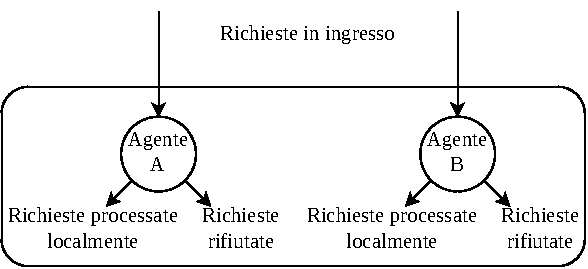
\includegraphics[width=\linewidth]{assets/4/1_sym_no_fw.pdf}
        \caption{Simmetrico senza inoltro}
    \end{subfigure}

    \begin{subfigure}{.6\textwidth}
        \centering
        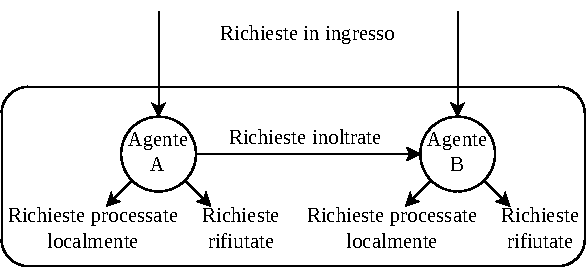
\includegraphics[width=\linewidth]{assets/4/2_asym.pdf}
        \caption{Asimmetrico}
    \end{subfigure}

    \begin{subfigure}{.6\textwidth}
        \centering
        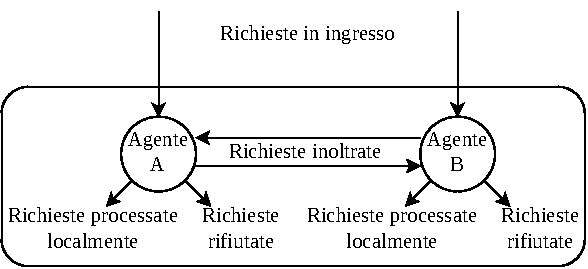
\includegraphics[width=\linewidth]{assets/4/3_sym_fw.pdf}
        \caption{Simmetrico con inoltro}
    \end{subfigure}
    
    \caption{I tre ambienti progettati con due agenti ciascuno.}
    \label{fig:4_environments}
\end{figure}

In ogni passo, ogni agente dell'ambiente agisce in un determinato spazio delle azioni, guidato dalle informazioni contenute nello spazio delle osservazioni. In risposta all'azione, l'ambiente restituisce agli agenti una ricompensa, calcolata dalla funzione di ricompensa. Le seguenti tre sottosezioni definiscono in modo formale i tre elementi.

\subsection{Spazio delle azioni}

La decisione consiste nel numero di richieste da processare localmente, inoltrare e rifiutare. Formalmente, si considera uno spazio di azioni continuo $\mathcal{A}$ i cui elementi sono delle tuple $(p^\textnormal{L}, p^\textnormal{F}, p^\textnormal{R})$, ogni $p^x$ è la percentuale di richieste da processare, inoltrare e rifiutare. Le percentuali fanno riferimento al numero di richieste in ingresso, informazione contenuta nello spazio delle osservazioni.

Per gli ambienti simmetrici senza inoltro e asimmetrici, lo spazio si riduce a tuple $(p^\textnormal{L}, p^\textnormal{R})$ per gli agenti che non possono inoltrare le richieste.

\subsubsection{Distribuzione di Dirichlet}

Un vincolo importante per lo spazio delle azioni è che un'azione $a \in \mathcal{A}$ soddisfi il vincolo

\begin{equation}\label{eq:4_simplex_condition}
    p^\textnormal{L} + p^\textnormal{F} + p^\textnormal{R} = 1.
\end{equation}

Analogamente, le azioni degli agenti che non possono inoltrare devono soddisfare $p^\textnormal{L} + p^\textnormal{R} = 1$. Il motivo è che, come introdotto sopra, le azioni rappresentano la percentuale (o proporzione) di richieste da distribuire nei modi definiti, pertanto tutte e sole le richieste devono essere distribuite.

\paragraph{Il simplesso.} Il vincolo in \Cref{eq:4_simplex_condition} può essere rappresentato con un \mbox{2-simplesso}, cioè un triangolo equilatero con vertici $(1, 0, 0), (0, 1, 0), (0, 0, 1) \in \mathbb{R}^3$. Ciascun asse rappresenta una delle tre azioni possibili. Ogni punto all'interno o sulla superficie del triangolo soddisfa il vincolo in \Cref{eq:4_simplex_condition}. La \Cref{fig:4_simplex} mostra il 2-simplesso con esempi di punti presi all'interno dello spazio.

Il simplesso definisce dei limiti precisi in cui l'agente può prendere le decisioni, garantendo che la somma delle azioni copra l'intero insieme delle richieste in ingresso. I vertici del simplesso indicano delle azioni ``estreme'': con $(1, 0, 0)$ l'agente elabora tutte le richieste localmente, con $(0, 1, 0)$ l'agente inoltra tutte le richieste e con $(0, 0, 1)$ l'agente rifiuta tutte le richieste.

\paragraph{La distribuzione.} Gli algoritmi di RL progettati per spazi d'azione continui, come in questo problema, non possono generare una policy imparando la probabilità di selezionare un'azione specifica nello stato attuale, come viene solitamente fatto quando $\mathcal{A}$ è un insieme finito (e non eccessivamente grande). Invece, gli agenti imparano ad approssimare, dallo stato attuale, i parametri di una distribuzione di probabilità sulle azioni, e l'azione scelta viene estratta da questa distribuzione. Per questo motivo è stata scelta la distribuzione di probabilità di Dirichlet, rispetto alle distribuzioni Gaussiana e Gaussiana-softmax: la prima, tipicamente adottata come distribuzione predefinita nell'algoritmo PPO, non garantisce che le azioni soddisfano il vincolo in \Cref{eq:4_simplex_condition}, mentre la seconda introduce un bias per via della normalizzazione e una maggiore varianza durante l'addestramento, oltre a una convergenza più lenta rispetto a Dirichlet \cite{Tian2022}.

\paragraph{Parametri della distribuzione.} Nel problema specifico, la distribuzione è parametrizzata dal numero di categorie $K$ e da un vettore di concentrazione $\boldsymbol{\alpha} = (\alpha_1, ..., \alpha_K)$. Ogni elemento $\alpha_i$ è un reale positivo e specifica la forma della distribuzione per la singola dimensione: se il valore di $\alpha_i$ è più alto degli altri, i valori estratti dalla distribuzione tendono a preferire la $i$-esima categoria. 

Nel problema specifico, $K = 3$ rimane costante poiché le azioni sono tre, mentre gli agenti imparano il vettore di concentrazione. Lo stesso vale per gli agenti che non possono inoltrare, in cui però $K = 2$.

\begin{figure}
    \centering

    \begin{subfigure}{.45\textwidth}
        \centering
        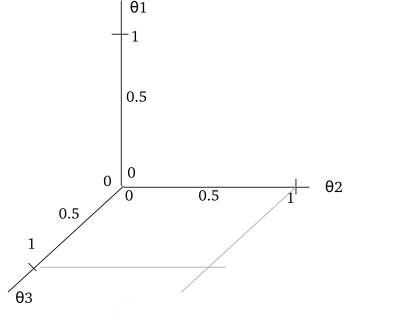
\includegraphics[width=\linewidth]{assets/4/simplex_1.png}
        \caption{}
        \label{fig:4_simplex_1}
    \end{subfigure}%
    \begin{subfigure}{.45\textwidth}
        \centering
        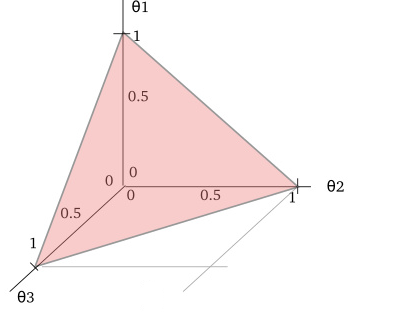
\includegraphics[width=\linewidth]{assets/4/simplex_2.png}
        \caption{}
        \label{fig:4_simplex_2}
    \end{subfigure}

    \begin{subfigure}{.45\textwidth}
        \centering
        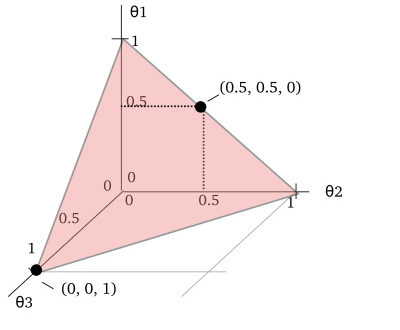
\includegraphics[width=\linewidth]{assets/4/simplex_3.png}
        \caption{}
        \label{fig:4_simplex_3}
    \end{subfigure}%
    \begin{subfigure}{.45\textwidth}
        \centering
        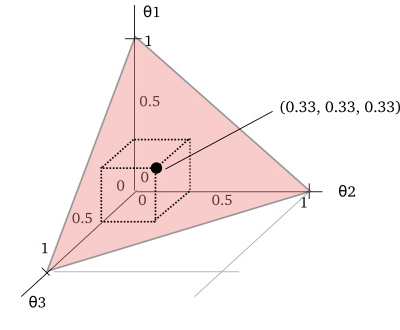
\includegraphics[width=\linewidth]{assets/4/simplex_4.png}
        \caption{}
        \label{fig:4_simplex_4}
    \end{subfigure}

    \begin{subfigure}{.9\textwidth}
        \centering
        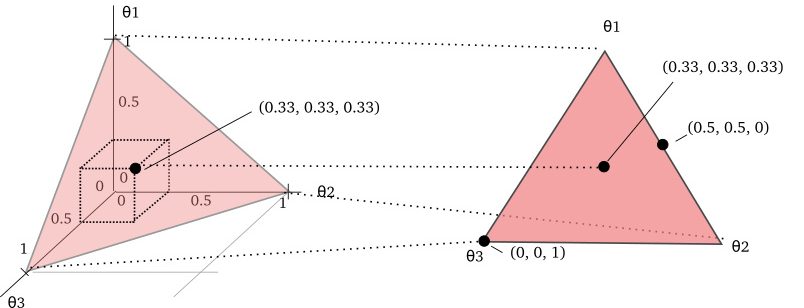
\includegraphics[width=\linewidth]{assets/4/simplex_5.png}
        \caption{}
        \label{fig:4_simplex_5}
    \end{subfigure}

    \caption[Esempio di 2-simplesso]{L'esempio mostra lo spazio tridimensionale con $\theta_{1, 2, 3}$ come coordinate, ogni coordinata può assumere valori nell'intervallo $[0, 1] \in \mathbb{R}$ (\Cref{fig:4_simplex_1}). \Cref{fig:4_simplex_2} mostra il 2-simplesso sullo spazio. \Cref{fig:4_simplex_3,fig:4_simplex_4} mostrano tre esempi di punti sul simplesso per cui vale il vincolo $\theta_1 + \theta_2 + \theta_3 = 1$. Infine \Cref{fig:4_simplex_5} mostra la proiezione del simplesso su due dimensioni con i punti mostrati in precedenza. Fonte: \url{https://stats.stackexchange.com/a/296779}}
    \label{fig:4_simplex}
\end{figure}

\begin{figure}
    \centering
    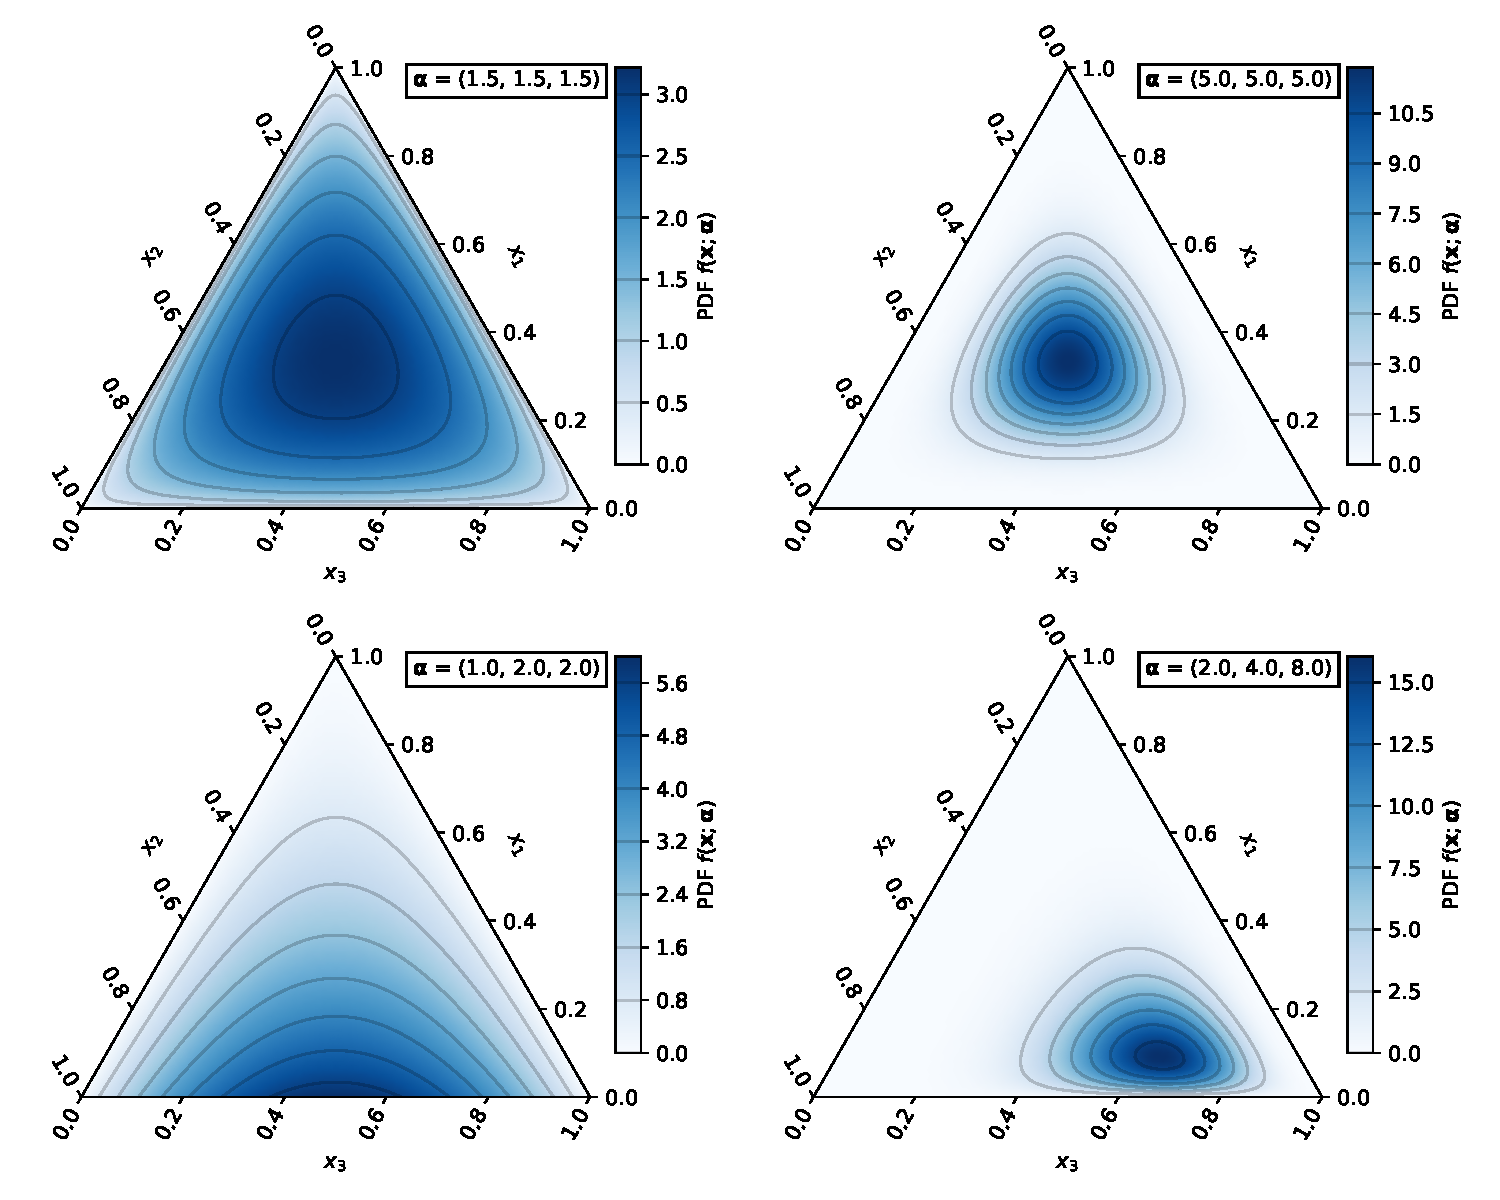
\includegraphics[width=\linewidth]{assets/4/dirichlet_concentration.pdf}
    \caption[Esempio di variazione dei parametri di concentrazione per Dirichlet]{Esempio di funzioni di densità di probabilità per le distribuzioni Dirichlet sul 2-simplesso al variare dei parametri di concentrazione. I valori delle funzioni sono mostrati dal colore con le linee di contorno che corrispondono al valore indicato nelle barre laterali. Fonte: Nerebur, CC BY-SA, Wikipedia Commons.}
    \label{fig:4_dirichlet_concentration}
\end{figure}

\subsection{Spazio delle osservazioni}

Ogni agente osserva uno stato $s \in \mathcal{S}$ definito dalla tupla $s = (R^\textnormal{IN}, q^\textnormal{FREE}, s^\textnormal{F}, s^\textnormal{FR})$: $R^\textnormal{IN}$ è il numero di richieste in ingresso, $q^\textnormal{FREE}$ è il numero di slot disponibili della coda per processare localmente le richieste, $s^\textnormal{F}$ sono il numero richieste inoltrate al passo precedente e $s^\textnormal{FR}$ sono le richieste inoltrate ma rifiutate nel passo precedente. Valgono sempre le seguenti condizioni: $R^\textnormal{IN} \ge 0$ e $s^\textnormal{FR} \le s^\textnormal{F}$.

Per l'ambiente asimmetrico e simmetrico senza inoltro, alcuni agenti non possono inoltrare le richieste e lo spazio si riduce a una tupla $s = (R^\textnormal{IN}, q^\textnormal{FREE})$.

\paragraph{Coda locale.} La gestione del carico all'interno di un singolo nodo avviene con una dinamica semplificata: la coda per l'elaborazione locale si svuota completamente a ogni passo, e diamo priorità alle richieste locali prima di gestire le richieste inoltrate ricevute da altri nodi. Quest'ultimo comportamento è stato scelto per essere più simile a come funziona DFaaS. Per questo motivo $q^\textnormal{FREE}$ nello stato coincide con $q^\textnormal{FREE}$. 

\subsection{Funzioni di ricompensa}
\label{sec:4_funzione_ricompensa}

La funzione di ricompensa è l'elemento essenziale per guidare gli agenti nel processo di apprendimento della strategia ottimale per distribuire le richieste in ingresso. Sono state definite due distinte funzioni di ricompensa una per gli agenti che non possono inoltrare le richieste e una per gli agenti che possono inoltrare. L'obiettivo comune di entrambe, ad alto livello, è di incentivare l'elaborazione locale delle richieste entro i limiti consentiti dalla capacità residua della coda, per poi inoltrare le richieste in eccesso che possono essere gestite dai nodi vicini, e infine rifiutare le richieste che non è possibile processare o inoltrare.

Per comodità, nelle funzioni di ricompensa non si utilizzano i valori percentuali $(p^\textnormal{L}, p^\textnormal{F}, p^\textnormal{R})$ che corrispondono direttamente all'azione scelta dall'agente, ma valori assoluti, definiti sulla base del carico in ingresso come $r^\textnormal{L} = R^\textnormal{IN} p^\textnormal{L}$, $r^\textnormal{F} = R^\textnormal{IN} p^\textnormal{F}$ e $r^\textnormal{R} = R^\textnormal{IN} p^\textnormal{R}$, per cui $r^\textnormal{L} + r^\textnormal{F} + r^\textnormal{R} = R^\textnormal{IN}$.

\subsubsection{Funzione senza inoltro}
\label{sec:4_reward_no_fw}

La funzione di ricompensa per l'agente in grado solo di processare localmente e rifiutare è definita come:

\begin{equation}
    \mathcal{R}: \mathbb{N}^0 \times \mathbb{N}^0 \times \mathbb{N}^0 \times \mathbb{N}^0 \times \mathbb{N}^0 \longrightarrow [0, 1], \quad 
    r_t = \mathcal{R}(r^\textnormal{L}, r^\textnormal{F}, e^\textnormal{R}, q^\textnormal{FREE}, q^\textnormal{MAX})
\end{equation}

in cui tutte le variabili, a eccezione di $q^\textnormal{MAX}$ che è costante, fanno riferimento a uno specifico agente per il $t$-esimo passo, ottenendo la ricompensa $r_t$.

La variabile $r^\textnormal{L}$ conteggia le richieste che l'agente vuole processare localmente. Tale numero può eccedere il numero di slot disponibili nella coda, perciò l'effettivo numero di richieste processate localmente è $r^\textnormal{L} - e^\textnormal{L}$ e che $e^\textnormal{L} \le r^\textnormal{L}$ è sempre soddisfatta.

La definizione segue $\mathcal{R}(s_t, a_t, s_{t+1})$ introdotta in \Cref{sec:2_reward_function_def} per un processo decisionale di Markov, poiché le variabili sopracitate sono sufficienti per racchiudere l'azione dell'agente, lo stato attuale e successivo dell'ambiente. Infatti dall'azione in valori assoluti si può ricavare il numero di richieste totali, mentre per la coda, poiché si svuota a ogni passo, è sufficiente conoscere lo stato ($q^\textnormal{FREE}$) a seguito della distribuzione delle richieste.

La funzione è composta da quattro casi:

\begin{enumerate}
    \item Se $R^\textnormal{IN} = 0$: caso base in cui la ricompensa è $r_t = 1$, in assenza di richieste da distribuire\footnote{Poiché $r^\textnormal{L}$ e $r^\textnormal{R}$ sono valori assoluti, si può ottenere $R^\textnormal{IN} = r^\textnormal{L} + r^\textnormal{R}$.}.

    \item Se $e^\textnormal{L} > 0$, l'agente ha cercato di processare localmente più richieste della capacità della coda. Più è alto il valore e si riduce la ricompensa, mostrata in \Cref{fig:4_reward_asym_no_fw_only_local}, per cui

    \begin{equation}
        r_t = 1 - \frac{e^\textnormal{L}}{r^\textnormal{L}}.
    \end{equation}

    \item Se $q^\textnormal{FREE} > r^\textnormal{R}$, la capacità residua della coda sarebbe stata sufficiente per processare tutte le richieste che l'agente ha scelto di rifiutare. Più è alta questo rapporto e più viene penalizzata la ricompensa, mostrata in \Cref{fig:4_reward_asym_no_fw_total_reject}, per cui:

    \begin{equation}
        r_t = 1 - \frac{r^\textnormal{R}}{R^\textnormal{IN}}.
    \end{equation}

    \item Se $q^\textnormal{FREE} \le r^\textnormal{R}$, invece ,alcune richieste potevano essere processate localmente, mentre le restanti sono state correttamente rifiutate. Solo le prime vengono penalizzate, come mostrato sempre \Cref{fig:4_reward_asym_no_fw_total_reject}, per cui:

    \begin{equation}
        r_t = 1 - \frac{q^\textnormal{FREE}}{R^\textnormal{IN}}.
    \end{equation}
\end{enumerate}

I quattro casi costituiscono la funzione completa:

\begin{equation}
    \mathcal{R}(\cdot) = \begin{dcases}
        1 & R^\textnormal{IN} = 0 \\
        1 - \frac{e^\textnormal{L}}{r^\textnormal{L}} & e^\textnormal{L} > 0 \\
        1 - \frac{r^\textnormal{R}}{R^\textnormal{IN}} & q^\textnormal{FREE} > r^\textnormal{R} \\
        1 - \frac{q^\textnormal{FREE}}{R^\textnormal{IN}} & q^\textnormal{FREE} \le r^\textnormal{R}
    \end{dcases}
\end{equation}

\begin{figure}
    \centering

    \begin{subfigure}{.7\textwidth}
        \centering
        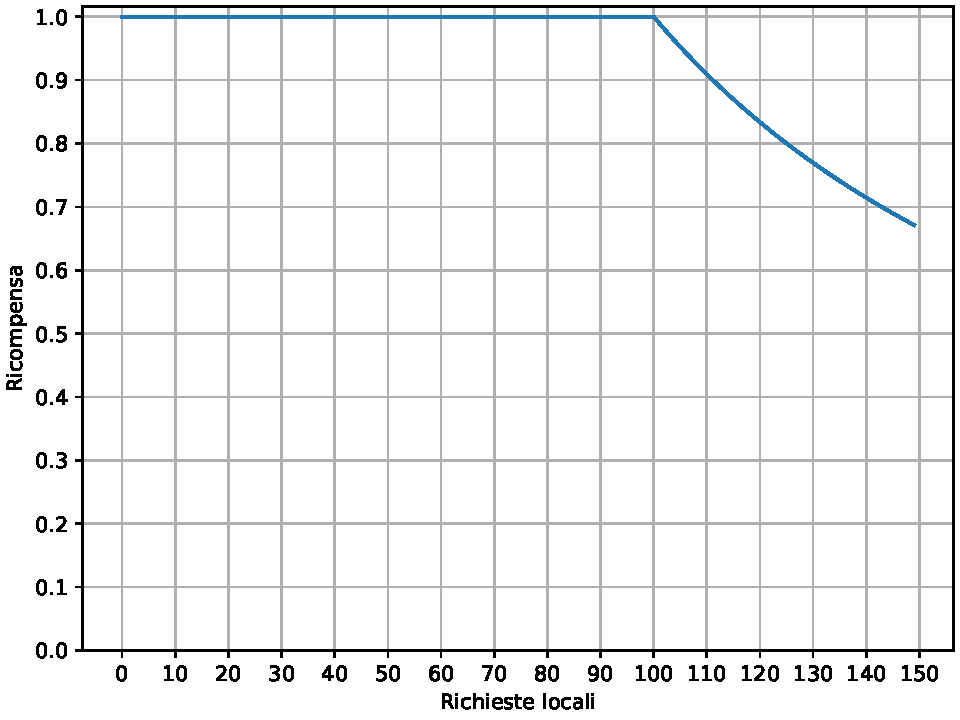
\includegraphics[width=\linewidth]{assets/4/reward_asym_no_forward_local_reqs.pdf}
        \caption{Ricompensa al variare delle richieste processate localmente ($r^\textnormal{R} = 0$).}
        \label{fig:4_reward_asym_no_fw_only_local}
    \end{subfigure}

    \begin{subfigure}{.7\textwidth}
        \centering
        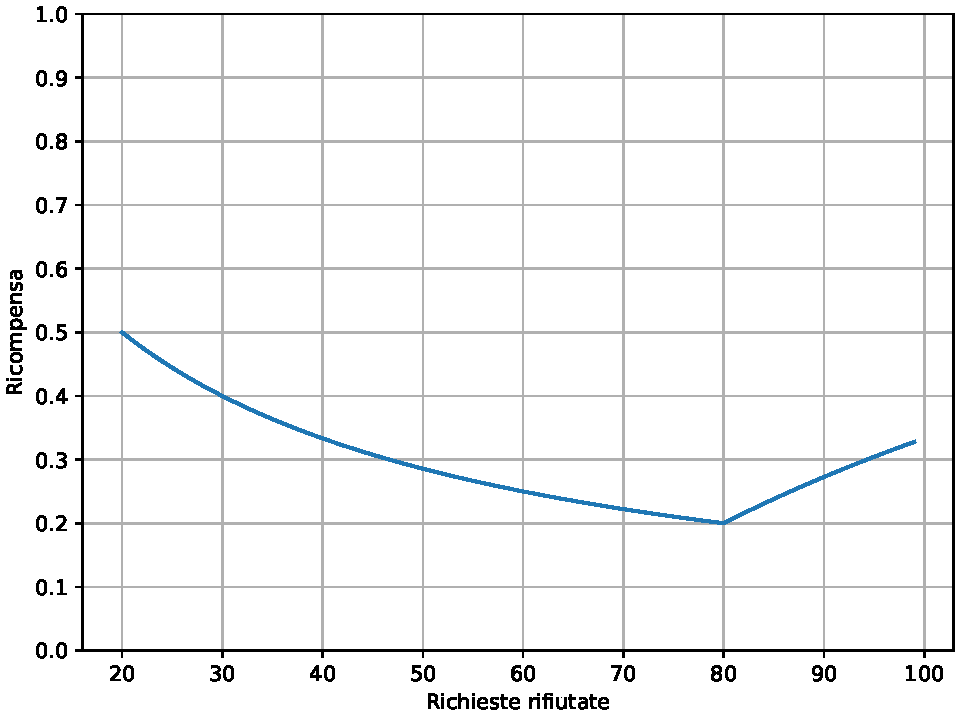
\includegraphics[width=\linewidth]{assets/4/reward_asym_no_forward_total_reject.pdf}
        \caption{Ricompensa al variare delle richieste rifiutate (${r^\textnormal{L} = 20}$). Per $r^\textnormal{R} \le 80$, avendo disponibilità di slot in coda, l'agente avrebbe dovuto processare tutte le richieste localmente. Per $r^\textnormal{R} > 80$, una porzione delle richieste sono inevitabilmente da rifiutare.}
        \label{fig:4_reward_asym_no_fw_total_reject}
    \end{subfigure}
    
    \caption[Esempi di ricompense per la funzione senza inoltro]{Esempi di ricompense per la funzione senza inoltro considerando $q^\textnormal{MAX} = 100$.}
    \label{fig:4_reward_asym_no_fw}
\end{figure}

\subsubsection{Funzione con inoltro}

La funzione di ricompensa per l'agente che è in grado di inoltrare è definita su

\begin{equation}
    \begin{gathered}
        \mathcal{R}^\textnormal{FW}: \mathbb{N}^0 \times \mathbb{N}^0 \times \mathbb{N}^0 \times \mathbb{N}^0 \times \mathbb{N}^0 \times \mathbb{N}^0 \times \mathbb{N}^0 \longrightarrow [0, 1], \\ r_t = \mathcal{R}^\textnormal{FW}(r^\textnormal{L}, r^\textnormal{F}, r^\textnormal{R}, e^\textnormal{L}, e^\textnormal{FR}, q^\textnormal{FREE}, q^\textnormal{MAX}),
    \end{gathered}
\end{equation}

in cui, come per la funzione precedente, tutte le variabili, a eccezione di $q^\textnormal{MAX}$, fanno riferimento a uno specifico agente per il $t$-esimo passo, ottenendo la ricompensa $r_t$.

Per $r^\textnormal{F}$, vale la stessa osservazione della funzione precedente per $r^\textnormal{F}$: $r^\textnormal{F} - e^\textnormal{FR}$ sono l'effettivo numero di richieste inoltrate che sono state processate dagli altri agenti e $e^\textnormal{FR} \le r^\textnormal{F}$ è sempre soddisfatta.

Ad alto livello, il calcolo della ricompensa segue un'idea diversa rispetto a quella descritta in \Cref{sec:4_reward_no_fw}: vengono conteggiate le richieste considerate ``sbagliate'', cioè richieste in ingresso che sono state gestite in un modo non ottimale. All'aumentare di questo conteggio la ricompensa decresce.

Tralasciando il caso base ($R^\textnormal{IN} = 0$) in cui non ci sono richieste in ingresso da processare, le richieste sbagliate sono conteggiate dalla somma dei seguenti termini:

\begin{itemize}
    \item Le richieste locali in eccesso $e^\textnormal{L}$, che sono di conseguenza rifiutate.

    \item Le richieste inoltrate ma rifiutate $e^\textnormal{FR}$. Questo termine penalizza la ricompensa se l'agente inoltra richieste che eccedono le risorse degli altri agenti, un esempio è mostrato in \Cref{fig:4_reward_fw_forward_reject}. Le \Cref{fig:4_reward_fw_can_forward,fig:4_reward_fw_cant_forward} mostrano due casi speciali: il primo in cui è sconsigliato inoltrare richieste poiché l'unica a essere stata inoltrata risulta rifiutata, il secondo in cui è consigliato inoltrare perché non sono state esaurite le risorse dei nodi vicini.

    \item Le richieste inoltrate in eccesso $e^\textnormal{F}$ che potevano essere processate localmente perché erano disponibili slot nella coda. Sono considerate solo le richieste effettivamente processate dagli altri agenti ($r^\textnormal{F} - e^\textnormal{FR}$):

    \begin{equation}
        e^\textnormal{F} = \begin{dcases}
            r^\textnormal{F} - e^\textnormal{FR} & q^\textnormal{FREE} > (r^\textnormal{F} - e^\textnormal{FR}) \\
            q^\textnormal{FREE} & q^\textnormal{FREE} \le (r^\textnormal{F} - e^\textnormal{FR})
        \end{dcases}.
    \end{equation}

    \item Le richieste rifiutate in eccesso $e^\textnormal{RF}$ che potevano essere inoltrate ipotizzando di processare localmente le richieste inoltrate in eccesso (il termine $q^\textnormal{FREE} - e^\textnormal{F}$):

    \begin{equation}
        e^\textnormal{RF} = \begin{dcases}
            r^\textnormal{R} - (q^\textnormal{FREE} - e^\textnormal{F}) & e^\textnormal{FR} = 0 \textnormal{ e } (r^\textnormal{R} - (q^\textnormal{FREE} - e^\textnormal{F})) > 0  \\
            0 & \textnormal{altrimenti}
        \end{dcases}.
    \end{equation}

    \item Le richieste rifiutate in eccesso $e^\textnormal{R}$ che potevano essere processate localmente:

    \begin{equation}
        e^\textnormal{R} = \begin{dcases}
            r^\textnormal{R} & q^\textnormal{FREE} - e^\textnormal{F} > r^\textnormal{R} \\
            q^\textnormal{FREE} - e^\textnormal{F}) & q^\textnormal{FREE} - e^\textnormal{F} \le r^\textnormal{R}
        \end{dcases}.
    \end{equation}
\end{itemize}

La funzione completa è quindi calcolata come

\begin{equation}
    \mathcal{R}^\textnormal{FW}(\cdot) = \begin{dcases}
        1 & R^\textnormal{IN} = 0 \\
        1 - \frac{e^\textnormal{L} + e^\textnormal{F} + e^\textnormal{FR} + e^\textnormal{RF} + e^\textnormal{R}}{R^\textnormal{IN}} & R^\textnormal{IN} > 0
    \end{dcases}.
\end{equation}

\begin{figure}
    \centering

    \begin{subfigure}{.6\textwidth}
        \centering
        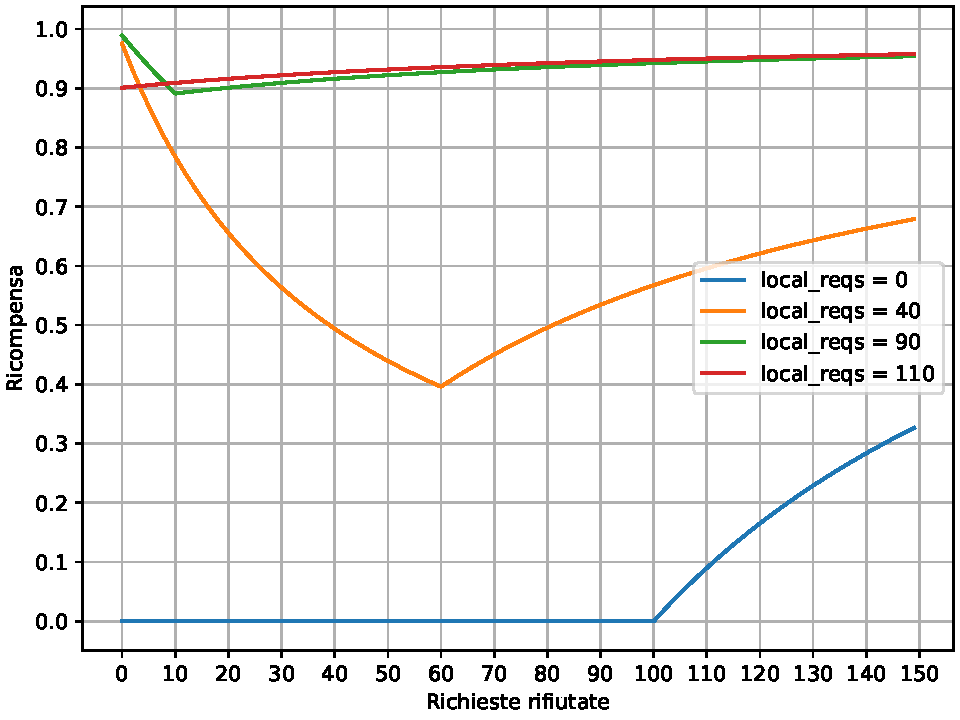
\includegraphics[width=\linewidth]{assets/4/reward_fw_cant_forward.pdf}
        \caption{Con $e^\textnormal{FR} = r^\textnormal{F} = 1$ non è possibile inoltrare richieste, il comportamento è simile alla funzione senza inoltro.}
        \label{fig:4_reward_fw_cant_forward}
    \end{subfigure}

    \begin{subfigure}{.6\textwidth}
        \centering
        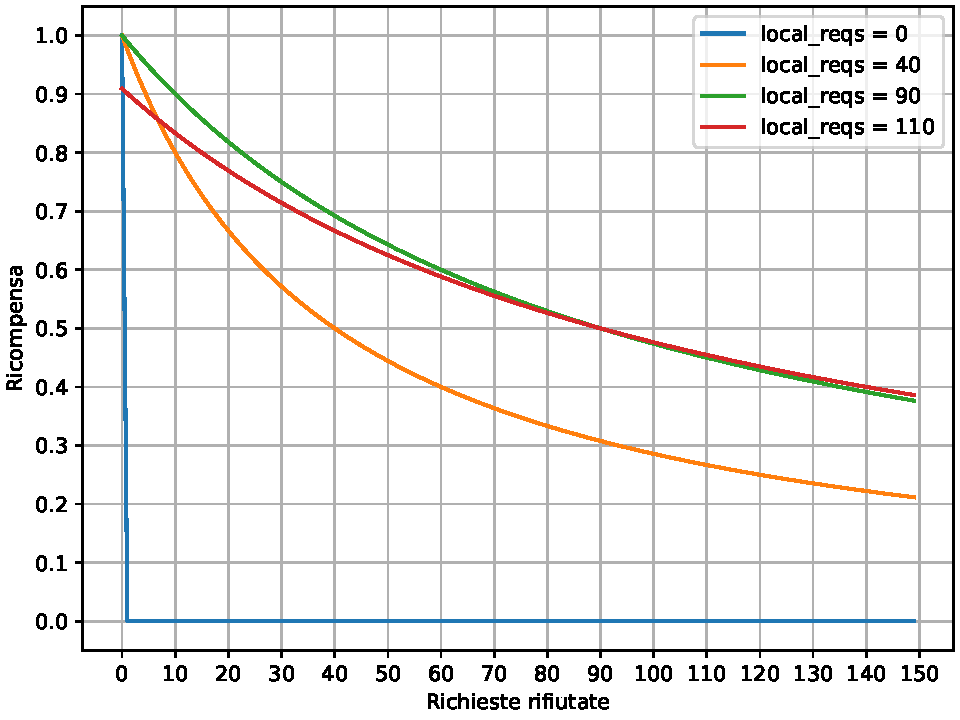
\includegraphics[width=\linewidth]{assets/4/reward_fw_can_forward.pdf}
        \caption{Con $e^\textnormal{FR} = r^\textnormal{F} = 0$ c'è sempre possibilità di inoltrare le richieste.}
        \label{fig:4_reward_fw_can_forward}
    \end{subfigure}

    \begin{subfigure}{.6\textwidth}
        \centering
        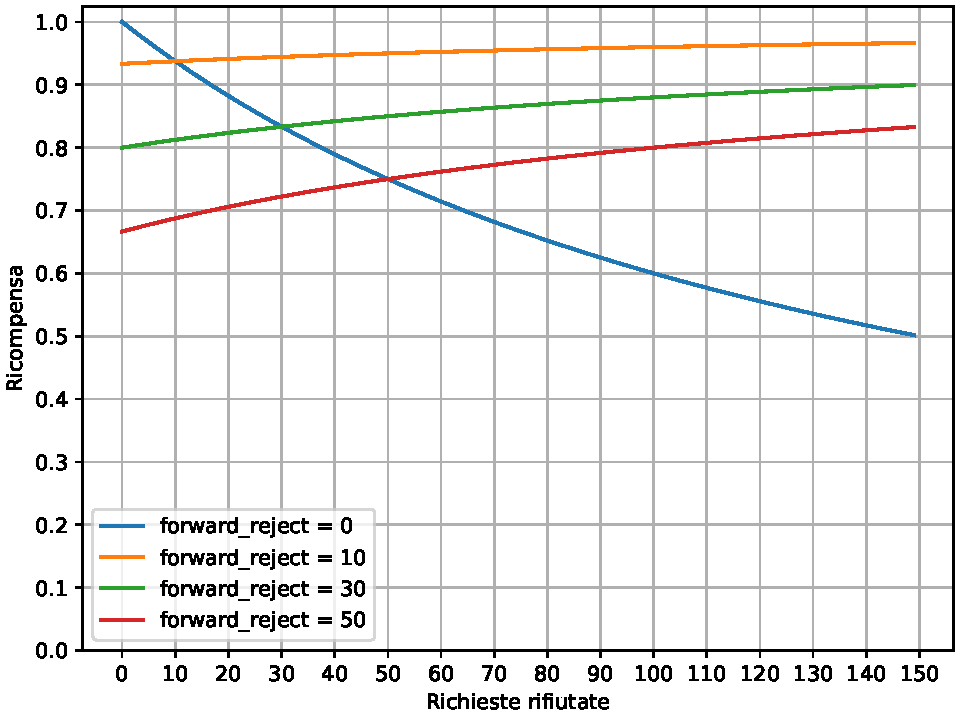
\includegraphics[width=\linewidth]{assets/4/reward_fw_forward_reject.pdf}
        \caption{Effetto del termine $e^\textnormal{FR}$ sulla ricompensa (${r^\textnormal{L} = 100}$, ${r^\textnormal{F} = 50}$).}
        \label{fig:4_reward_fw_forward_reject}
    \end{subfigure}
    
    \caption[Esempi di ricompense per la funzione con inoltro]{Esempi di ricompense per la funzione con inoltro considerando ${q^\textnormal{MAX} = 100}$.}
    \label{fig:4_reward_fw}
\end{figure}

\section{Dinamica degli ambienti}
\label{sec:4_dinamica_ambienti}

\paragraph{Ambienti episodici.} I tre ambienti sono di tipo episodici nonostante lo scenario reale di riferimento sia continuo. Tale scelta è rilevante solo per la sezione sperimentale, poiché agevola la gestione dell'ambiente durante la fasi di addestramento e valutazione; a livello teorico per il problema affrontato separare un ambiente continuo in episodico non perde di generalità.

L'episodio, nel problema affrontato, modella una giornata di 24 ore di distribuzione del carico. Ogni episodio dura esattamente 288 passi, un passo per 5 minuti che coprono l'arco della giornata. La scelta di considerare 5 minuti è motivata dal desiderio di dare tempo agli agenti, nel corrispettivo scenario reale, di reagire con maggiore robustezza ai cambiamenti nel carico su un periodo più esteso dei secondi o del singolo minuto.

\paragraph{Differenze dei tre ambienti.} Le differenze dei tre ambienti si concentrano sullo spazio delle azioni, osservazioni e funzione di ricompensa, poiché sono tre aspetti legati tra di loro. Solo gli ambienti BASE e SYM questi tre aspetti sono omogenei per tutti gli agenti, perché o tutti possono inoltrare o nessuno può; l'ambiente ASYM invece una parte degli agenti possono inoltrare e un'altra no.

Una differenza importante riguarda anche la gestione delle richieste inoltrate in ingresso da altri agenti: in ASYM e SYM le richieste di questo tipo sono elaborate localmente solo dopo aver elaborato le richieste in ingresso dirette per un nodo. In BASE questo meccanismo è assente, poiché nessun agente può inoltrare.

\paragraph{} Il funzionamento dell'ambiente segue le seguenti fasi:

\begin{enumerate}
    \item Inizializzazione: l'ambiente viene inizializzato con i valori di $q^\textnormal{MAX}$ per ogni agente, un contatore per il passo, il generatore di numeri pseudocasuali e la tipologia di carico in ingresso, con la scelta o generazione delle richieste (descritti nella \Cref{sec:5_scenari}).

    \item Azione: ogni agente sceglie un'azione $(p^\textnormal{L}, p^\textnormal{F}, p^\textnormal{R})$ di distribuzione del carico, in base all'osservazione ricevuta. L'ambiente converte i valori percentuali in assoluti sulla base del carico in ingresso per quel passo, ottenendo $(r^\textnormal{L}, r^\textnormal{F}, r^\textnormal{R})$.

    \item Gestione del carico: a partire dal numero di richieste da distribuire, per ogni agente l'ambiente processa le richieste locali occupando gli slot della coda locale. Inoltra le richieste, per gli agenti che sono in grado di inoltrare, e le richieste inoltrare in ingresso occupano gli slot con priorità secondaria rispetto alle richieste locali.

    \item Calcolo della ricompensa: l'ambiente, in base agli effetti dell'azione sullo stato, calcola la ricompensa per ogni agente.

    \item Avanzamento del passo: l'ambiente incrementa il contatore dei passi, svuota la coda locale e genera le nuove osservazioni da restituire agli agenti. Se non è l'ultimo passo, torna alla fase 2. 

    \item Conclusione dell'episodio: essendo l'ambiente episodico, al termine dell'ultimo passo viene restituito un segnale di terminazione all'agente e viene effettuato un ripristino dell'ambiente, tornando alla fase 1.
\end{enumerate}

\chapter{Sezione sperimentale}
\label{sec:5_esperimenti}

In questo capitolo viene presentata l'analisi sperimentale svolta per valutare l'approccio multi-agente proposto nella tesi. La prima sezione espone le scelte sperimentali adottate nell'implementazione degli ambienti e dell'algoritmo, oltre alla configurazione degli addestramenti e la presentazione delle metriche di valutazione. La seconda sezione invece presenta e analizza i risultati ottenuti.

\section{Tecnologie implementative}

Nell'implementazione ed esecuzione degli esperimenti sono state effettuate scelte tecnologiche per realizzare lo studio. La scelta più importante è stata l'uso di Python come linguaggio di programmazione, per via della sua popolarità nell'ambito del machine learning e nello specifico nell'apprendimento per rinforzo. È stata poi scelta la libreria RLlib, presentata in \cite{Liang2018}, come base da cui implementare gli ambienti ed eseguire gli esperimenti. RLlib\footnote{\url{https://docs.ray.io/en/latest/rllib/index.html}} è una libreria open source per l'apprendimento per rinforzo che implementa algoritmi ottimizzati per utilizzare accelerazione hardware, tramite il framework PyTorch introdotto da \cite{Ansel2024}. Rispetto ad altre librerie è stata preferita perché incorpora funzionalità che si adattano
allo scenario di FaaS decentralizzato: gli algoritmi sono implementati anche in versione decentralizzata, con la possibilità di sviluppare ambienti multi-agente. RLlib è basato su Ray \cite{Moritz2018}, un framework open source che supporta l'esecuzione decentralizzata e distribuita di applicazioni scritte in Python e dedicate al machine learning. È stata utilizzata nello specifico la versione 2.10.0 di RLlib. La \Cref{fig:5_ray_rllib_architecture} mostra l'architettura della libreria.

\begin{figure}[ht]
    \centering
    \includegraphics[width=.6\linewidth]{assets/5/ray_rllib_architecture.pdf}
    \caption[Architettura della libreria RLlib]{Architettura della libreria RLlib. Fonte: \url{https://docs.ray.io/en/latest/rllib/index.html}}
    \label{fig:5_ray_rllib_architecture}
\end{figure}

Gli ambienti sono stati implementati seguendo le API multi-agente definite da RLlib, a loro volta basate su Gymnasium, l'API standard de-facto per gli ambienti per l'apprendimento per rinforzo in Python, approfondita in \cite{Towers2024}.

Nell'implementazione sono state inoltre utilizzate le seguenti librerie: NumPy per la gestione degli array, presentata in \cite{Harris2020}, Pandas per la gestione dei dati nello scenario reale, presentata in \cite{Mckinney2010} e \cite{Pandas2024}, e Matplotlib per la produzione dei grafici presenti nel documento, introdotto in \cite{Hunter2007}.

\section{Configurazione e valutazione degli esperimenti}

L'obiettivo dell'analisi sperimentale è di validare la realizzabilità di un ambiente multi-agente per la distribuzione del carico con l'algoritmo PPO, nelle due modalità multi-agente descritte in \Cref{sec:2_rl_ppo_choices}. Nello specifico, l'analisi vuole dimostrare che, al crescere della complessità degli ambienti modellati nel \Cref{sec:4_modellazione}, ossia permettendo di inoltrare le richieste, gli agenti siano in grado di processare un maggior numero di richieste, a fronte di carichi in ingresso di natura diversa, le cui tipologie sono dettagliate nella sottosezione seguente. La configurazione degli esperimenti è stata attentamente progettata per assicurare risultati che siano coerenti e soprattutto riproducibili.

\subsection{Configurazione degli ambienti}

I tre ambienti modellati sono stati configurati nel seguente modo:

\begin{itemize}
    \item Ogni agente ha la stessa capacità di coda locale per ogni passo fissa a 100, per cui $q^\textnormal{MAX} \coloneqq 100$.

    \item Il carico $R^\textnormal{IN}$ in ingresso ad ogni agente $n \in \mathcal{N}$ al $t$-esimo passo può assumere valori nell'intervallo $[0, 150]$.

    \item Ogni ambiente ha due agenti $|\mathcal{N}| = 2$. Nel caso dell'ambiente asimmetrico, un agente può inoltrare, mentre l'altro può solo ricevere le richieste inoltrate.
\end{itemize}

La scelte di $q^\textnormal{MAX}$ e dell'intervallo di $R^\textnormal{IN}$ sono state effettuate sulla base di osservazioni empiriche per garantire dei carichi gestibili per i due agenti. Come anticipato nella \Cref{sec:4_dinamica_ambienti}, l'ambiente è di tipo episodico da 288 passi.

\subsection{Scenari}
\label{sec:5_scenari}

Nell'esecuzione degli esperimenti, per una successiva valutazione di PPO ad apprendere politiche ottimali di distribuzione, un passo importante è stata la scelta delle richieste da fornire in ingresso a ogni agente dell'ambiente, sia in fase di addestramento sia in fase di valutazione. Per tale scopo sono stati definiti tre scenari, caratterizzati dalla modalità di generazione delle richieste in ingresso. Il criterio di definizione ha l'obiettivo di presentare agli agenti scenari che esprimano situazioni multiformi, fornendo in questo modo una visione più ampia dei comportamenti appresi dall'algoritmo nelle situazioni proposte. Inoltre, gli scenari sono stati progettati cercando di sottoporre gli agenti a contesti di lavoro di varie difficoltà e forme. Nello specifico, gli scenari definiti sono:

\begin{itemize}
    \item \textbf{Scenario reale}: gli agenti sono sottoposti a carichi provenienti da dati reali di traffico in ingresso, selezionati ed elaborati come descritto nelle sezioni successive.

    \item \textbf{Scenari sintetici}: gli agenti sono sottoposti a carichi generati artificialmente che non hanno una corrispondenza reale ma sono costruiti con delle caratteristiche simili ai carichi reali. Sono stati definiti due scenari per questa tipologia:

        \begin{itemize}
            \item \textbf{Scenario sintetico sinusoidale}: ogni agente è sottoposto a un carico generato seguendo una forma sinusoidale, con l'aggiunta di rumore.

            \item \textbf{Scenario sintetico gaussiano}: ogni agente è sottoposto da un carico generato seguendo una distribuzione normale.
        \end{itemize}
\end{itemize}

Per la durata di un intero episodio, per ogni agente sono generate (o estratte in caso di scenario reale) tracce con in media \numprint{17000}-\numprint{18000} richieste. I tre scenari hanno le seguenti caratteristiche in comune: una media di richieste di circa 60 per passo, deviazione standard di 30 (solo per lo scenario sintetico gaussiano e reale) e di 60 (scenario sintetico sinusoidale), mentre la deviazione standard della somma delle richieste è di \numprint{7500} (scenario reale) e \numprint{750} (scenari sintetici). Sono pertanto scenari diversi che pongono sfide di natura diversa agli agenti.

È importante sottolineare che in ogni fase di addestramento vengono estratte delle tracce da uno scenario selezionato all'avvio dell'esperimento. Questo significa che non è stato previsto che un agente venga addestrato con tracce di uno scenario diverso dall'altro agente. Lo stesso avviene per la valutazione, con la differenza che un agente può essere valutato più volte selezionando scenari alternativi a quello di addestramento.

\subsubsection{Scenario reale}
\label{sec:5_scenario_reale}

Lo scenario reale è definito dall'uso del sottoinsieme di richieste pubblicate e analizzate in \cite{Shahrad2020} e rilasciate su GitHub\footnote{\url{https://github.com/Azure/AzurePublicDataset}}. Le richieste, o ``tracce'' seguendo la terminologia del set di dati considerato, sono un sottoinsieme registrato dal 15 al 28 Luglio 2019 sull'intera infrastruttura di Microsoft Azure Functions. Il dataset cattura il carico in ingresso FaaS caratterizzato dalle proprietà intrinseche delle applicazioni e delle funzioni, e non dalle caratteristiche della piattaforma sottostante. Questo ha permesso di utilizzare le richieste raccolte così come sono nell'ambiente DFaaS simulato. I dati raccolti e pubblicati comprendono informazioni su quante volte al minuto viene invocata una funzione e per quale categoria di trigger\footnote{I trigger sono la causa di esecuzione di una funzione, definiscono come una funzione viene invocata. Azure Functions supporta decine di trigger, ma nel set di dati sono raggruppati in 7 classi.}, come le funzioni sono organizzate in applicazioni e a quali utenti sono associate, la distribuzione dei tempi di esecuzione per funzione e la distribuzione dell'utilizzo della memoria per applicazione. Per lo studio esplorativo di questa tesi, sono state considerate solo le invocazioni causate dal trigger HTTP, perché sono le più affini all'architettura e funzionamento di DFaaS. Due esempi di questa tipologia di tracce sono mostrate in \Cref{fig:5_real_traces}.

\begin{figure}
    \centering

    \begin{subfigure}{.95\textwidth}
        \centering
        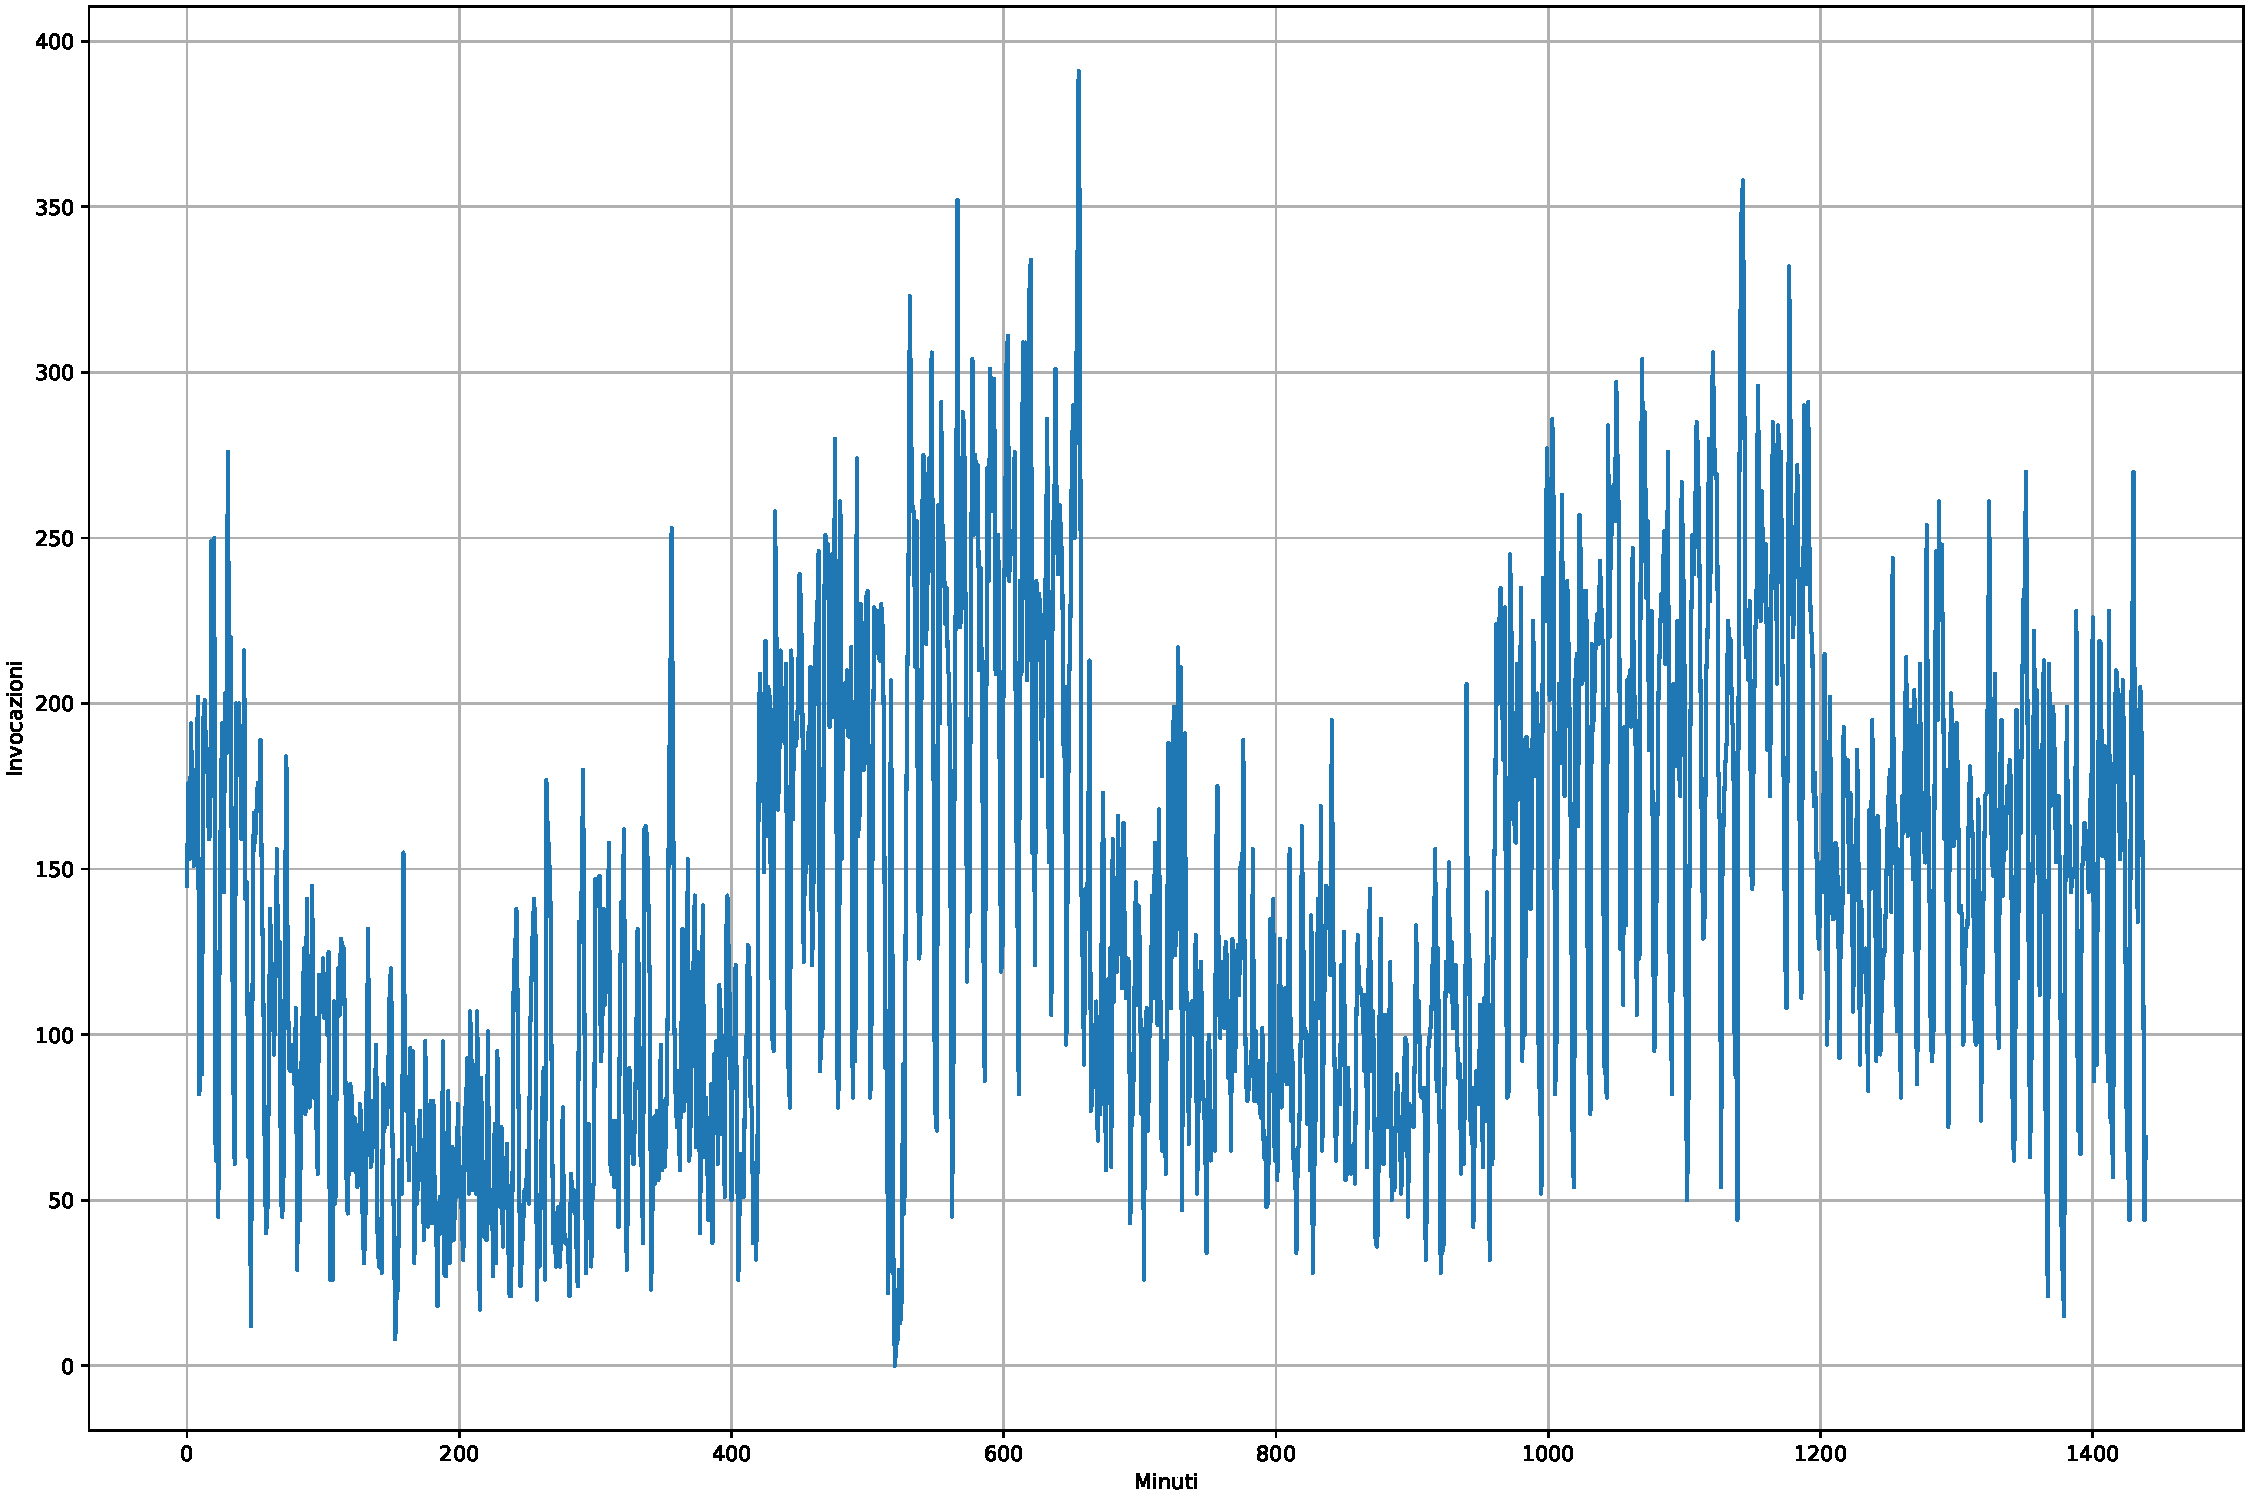
\includegraphics[width=\linewidth]{assets/5/requests_9dc54e.pdf}
        \caption{Traccia della funzione 9dc54e.}
        \label{fig:5_real_traces_9dc54e}
    \end{subfigure}

    \begin{subfigure}{.95\textwidth}
        \centering
        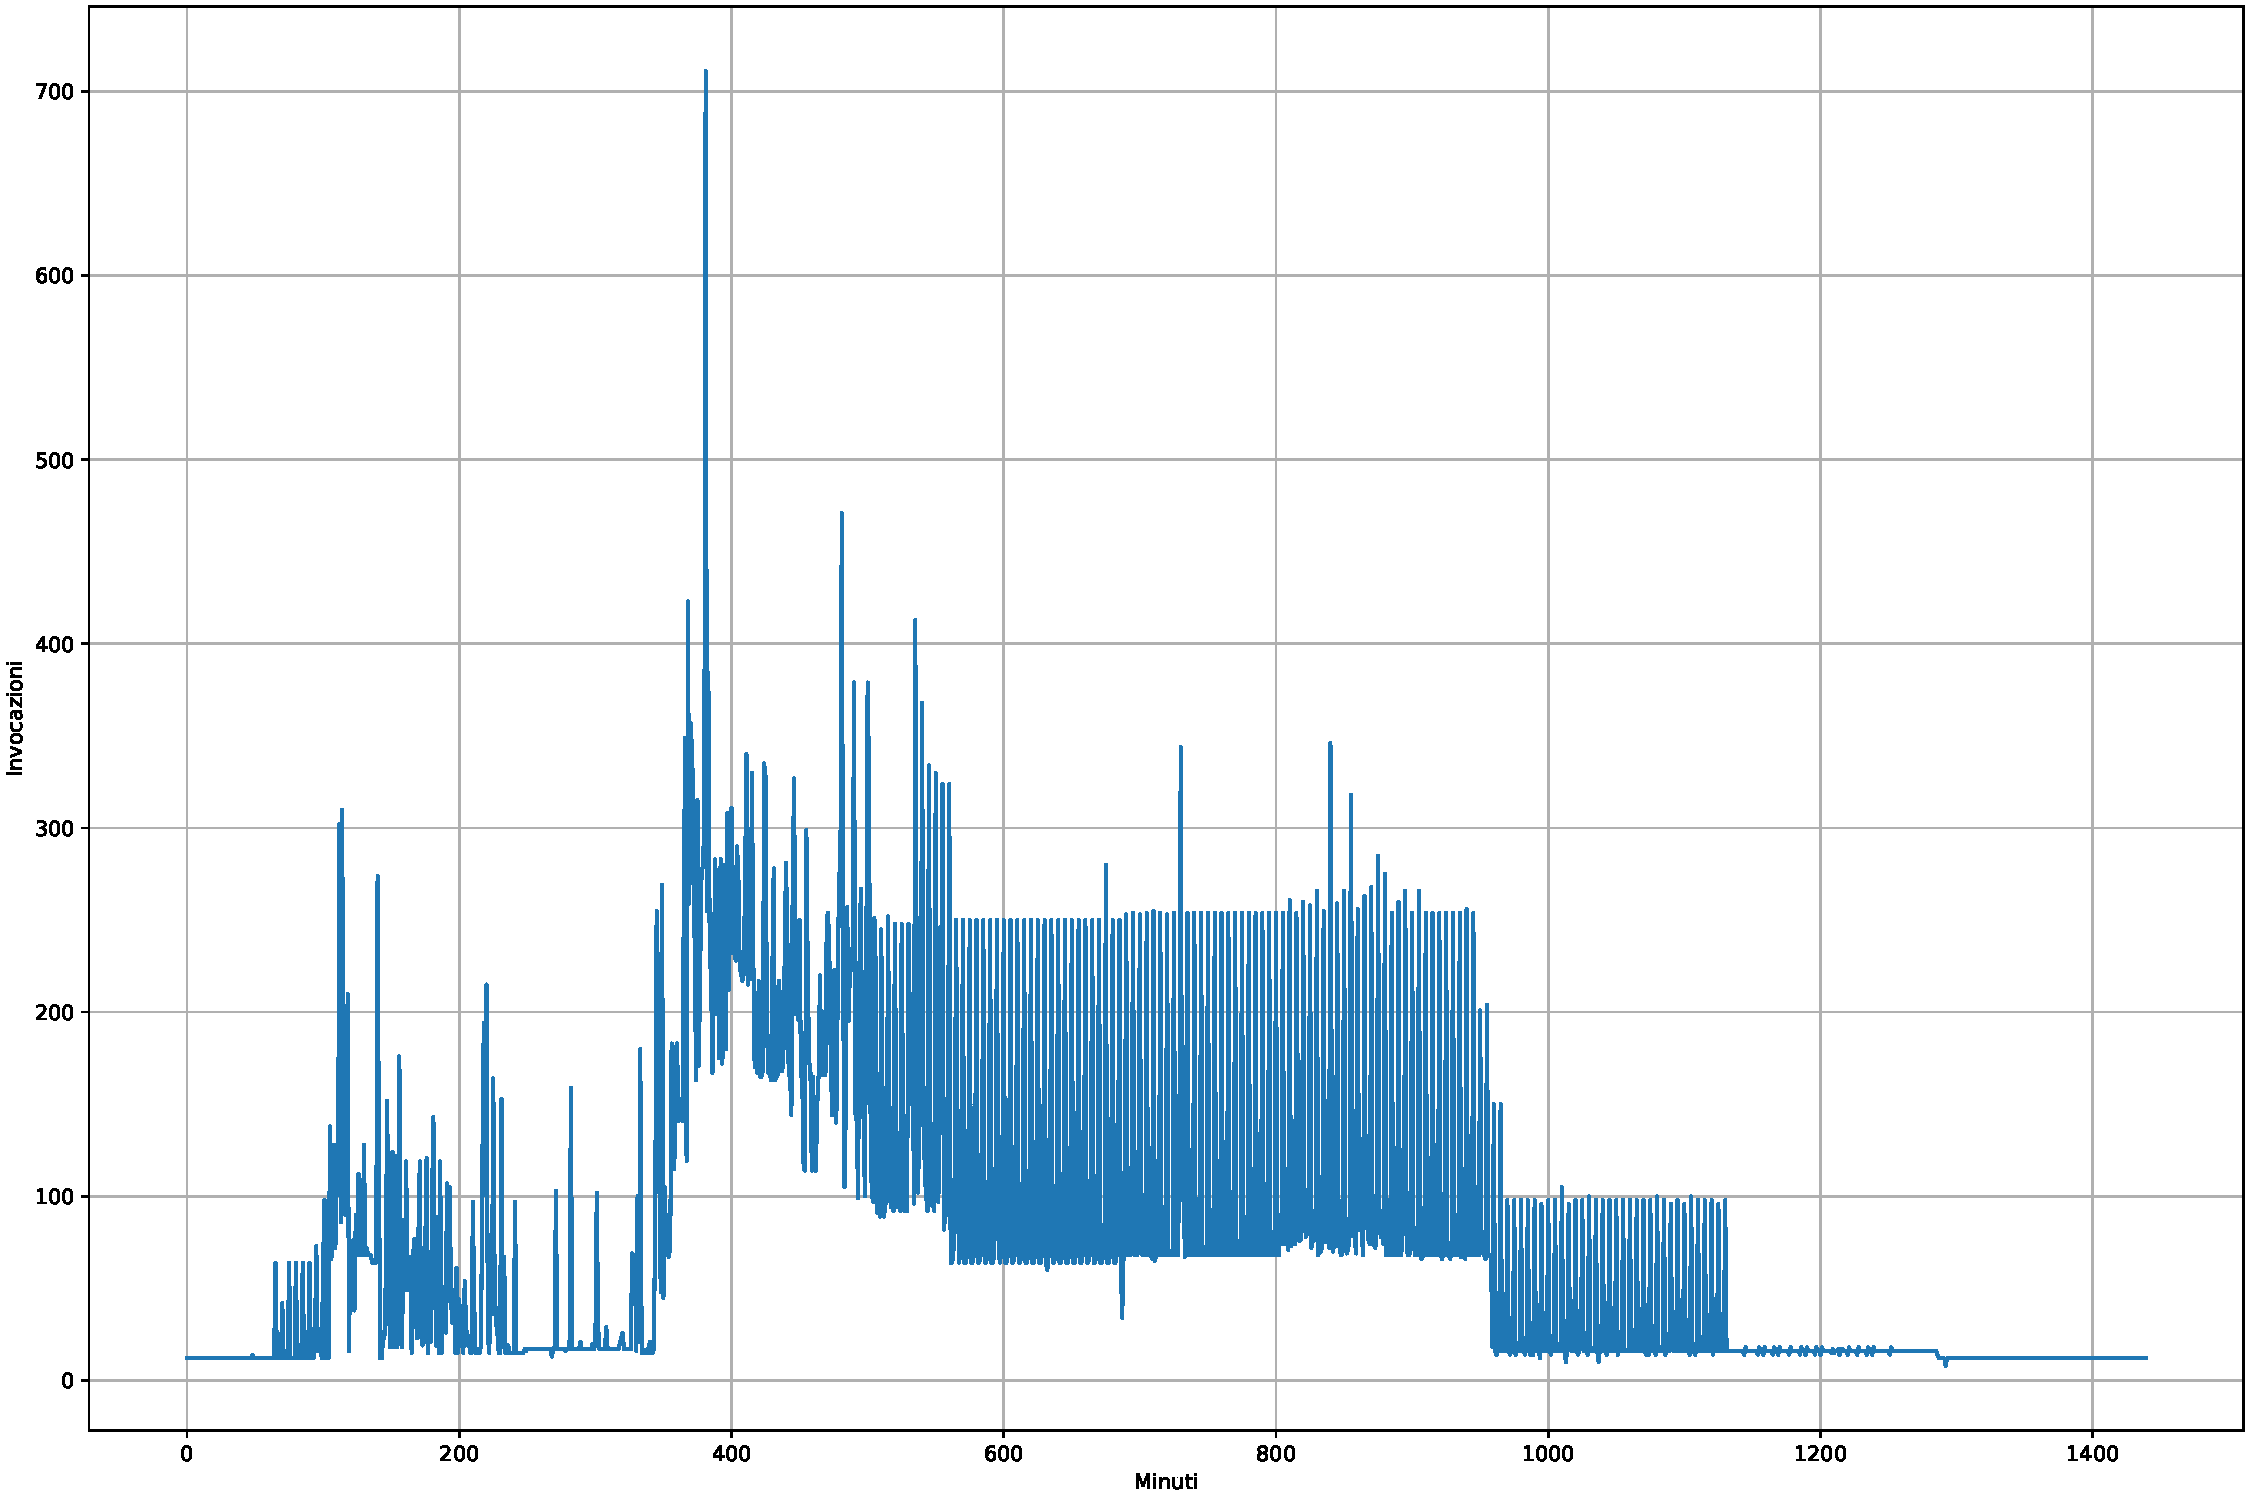
\includegraphics[width=\linewidth]{assets/5/requests_f2d88b.pdf}
        \caption{Traccia della funzione f2d88b.}
        \label{fig:5_real_traces_f2d88b}
    \end{subfigure}
    
    \caption[Esempio di invocazioni di due funzioni dal set di dati reale]{Esempio di invocazioni di due funzioni registrate il 15 Luglio 2019 e scatenate dal trigger HTTP. Per ognuna sono indicati gli ultimi tre byte dell'hash di identificazione.}
    \label{fig:5_real_traces}
\end{figure}

Il set di dati è costituito da 14 file in formato CSV, ognuno dei quali caratterizza le invocazioni relative a funzioni per un giorno preciso. Per ogni traccia registrata è presente l'identificativo della funzione, dell'applicazione e dell'utente (il proprietario). All'interno della piattaforma Azure Functions, le funzioni sono logicamente raggruppate in applicazioni, e un'applicazione può comprendere una o più funzioni. Un unico utente può essere legato a più di una applicazione. È importante sottolineare che funzioni identiche possono appartenere a diverse applicazioni, e una stessa applicazione a più utenti (ognuno dei quali con una propria copia). Il set di dati è stato reso anonimo processando tutti gli identificativi con HMAC-SHA256 e un salt\footnote{Una sequenza casuale di bit aggiunti alla funzione di hash per evitare che due stessi input vengano mappati allo stesso hash.} segreto diverso per ogni colonna. Di conseguenza due applicazioni identiche ma con diversi proprietari sono identificati da hash diversi, e lo stesso vale per due funzioni identiche che appartengono ad applicazioni diverse. Tuttavia gli hash sono coerenti nei file, è quindi possibile correlare funzioni, applicazioni e proprietari nell'intervallo dei giorni.

\paragraph{Processamento delle tracce.} Affinché le tracce reali potessero essere utilizzate per addestrare e valutare gli esperimenti, è stata svolta una procedura di selezione e ridimensionamento:

\begin{enumerate}
    \item A partire da \numprint{618559} tracce, distribuite nei 14 giorni di registrazione, sono state estratte le \numprint{200274} tracce con trigger HTTP.

    \item Le tracce selezionate sono state scalate da 1440 passi (1 minuto per 24 ore) a 288 (5 minuti per 24 ore) accorpando i valori ogni cinque passi, e normalizzate nei valori per rientrare nell'intervallo $[0, 150]$.
    
    \item Infine sono state selezionate \numprint{14775} tracce finali usate per addestrare e valutare gli esperimenti. La selezione è stata necessaria perché il set di dati contiene tracce di grande variabilità, per esempio con carichi molto bassi oppure al contrario eccessivamente alti, o carichi con troppa dispersione, che possono portare l'addestramento a modelli sub-ottimali. I criteri di selezione sono stati la media (valori compresi in $[30, 130]$) e la deviazione standard (valori compresi in $[10, 60]$).
\end{enumerate}

In \Cref{fig:5_real_traces_scaled} sono mostrate le tracce ridimensionate delle stesse funzioni in \Cref{fig:5_real_traces}. Al termine della selezione la funzione f2d88b è stata scartata poiché la deviazione standard è al di fuori dell'intervallo scelto.

\begin{figure}
    \centering

    \begin{subfigure}{.95\textwidth}
        \centering
        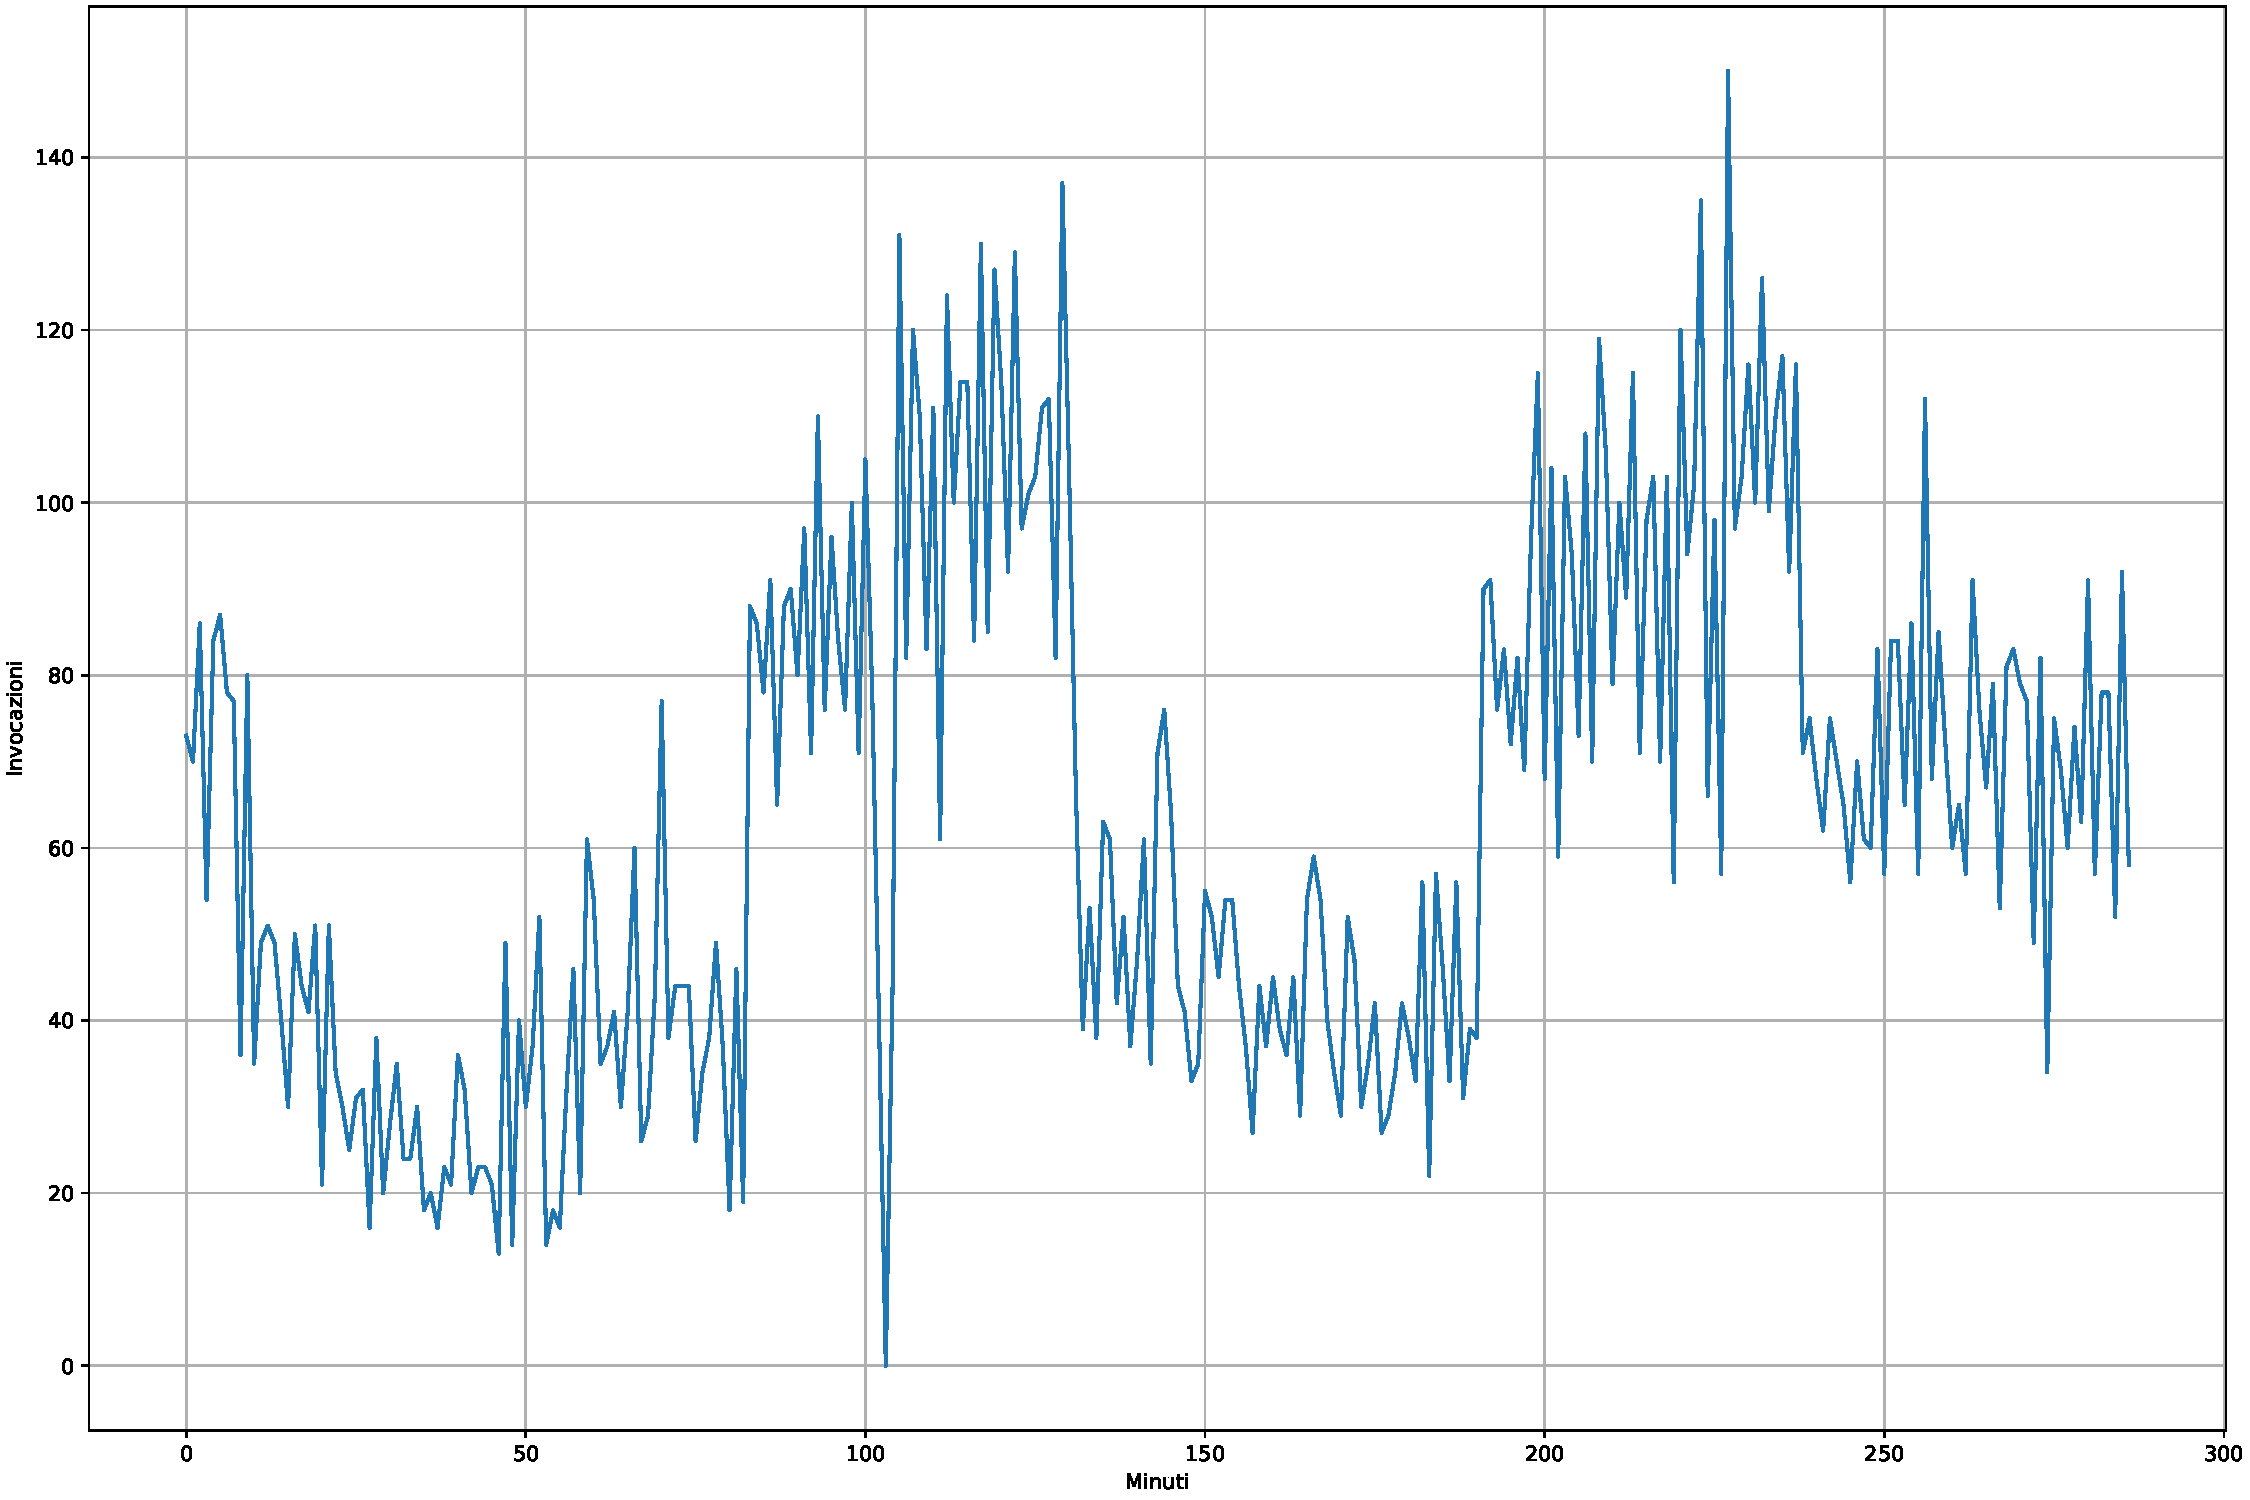
\includegraphics[width=\linewidth]{assets/5/requests_9dc54e_scaled.pdf}
        \caption{Traccia della funzione 9dc54e.}
        \label{fig:5_real_traces_scaled_9dc54e}
    \end{subfigure}

    \begin{subfigure}{.95\textwidth}
        \centering
        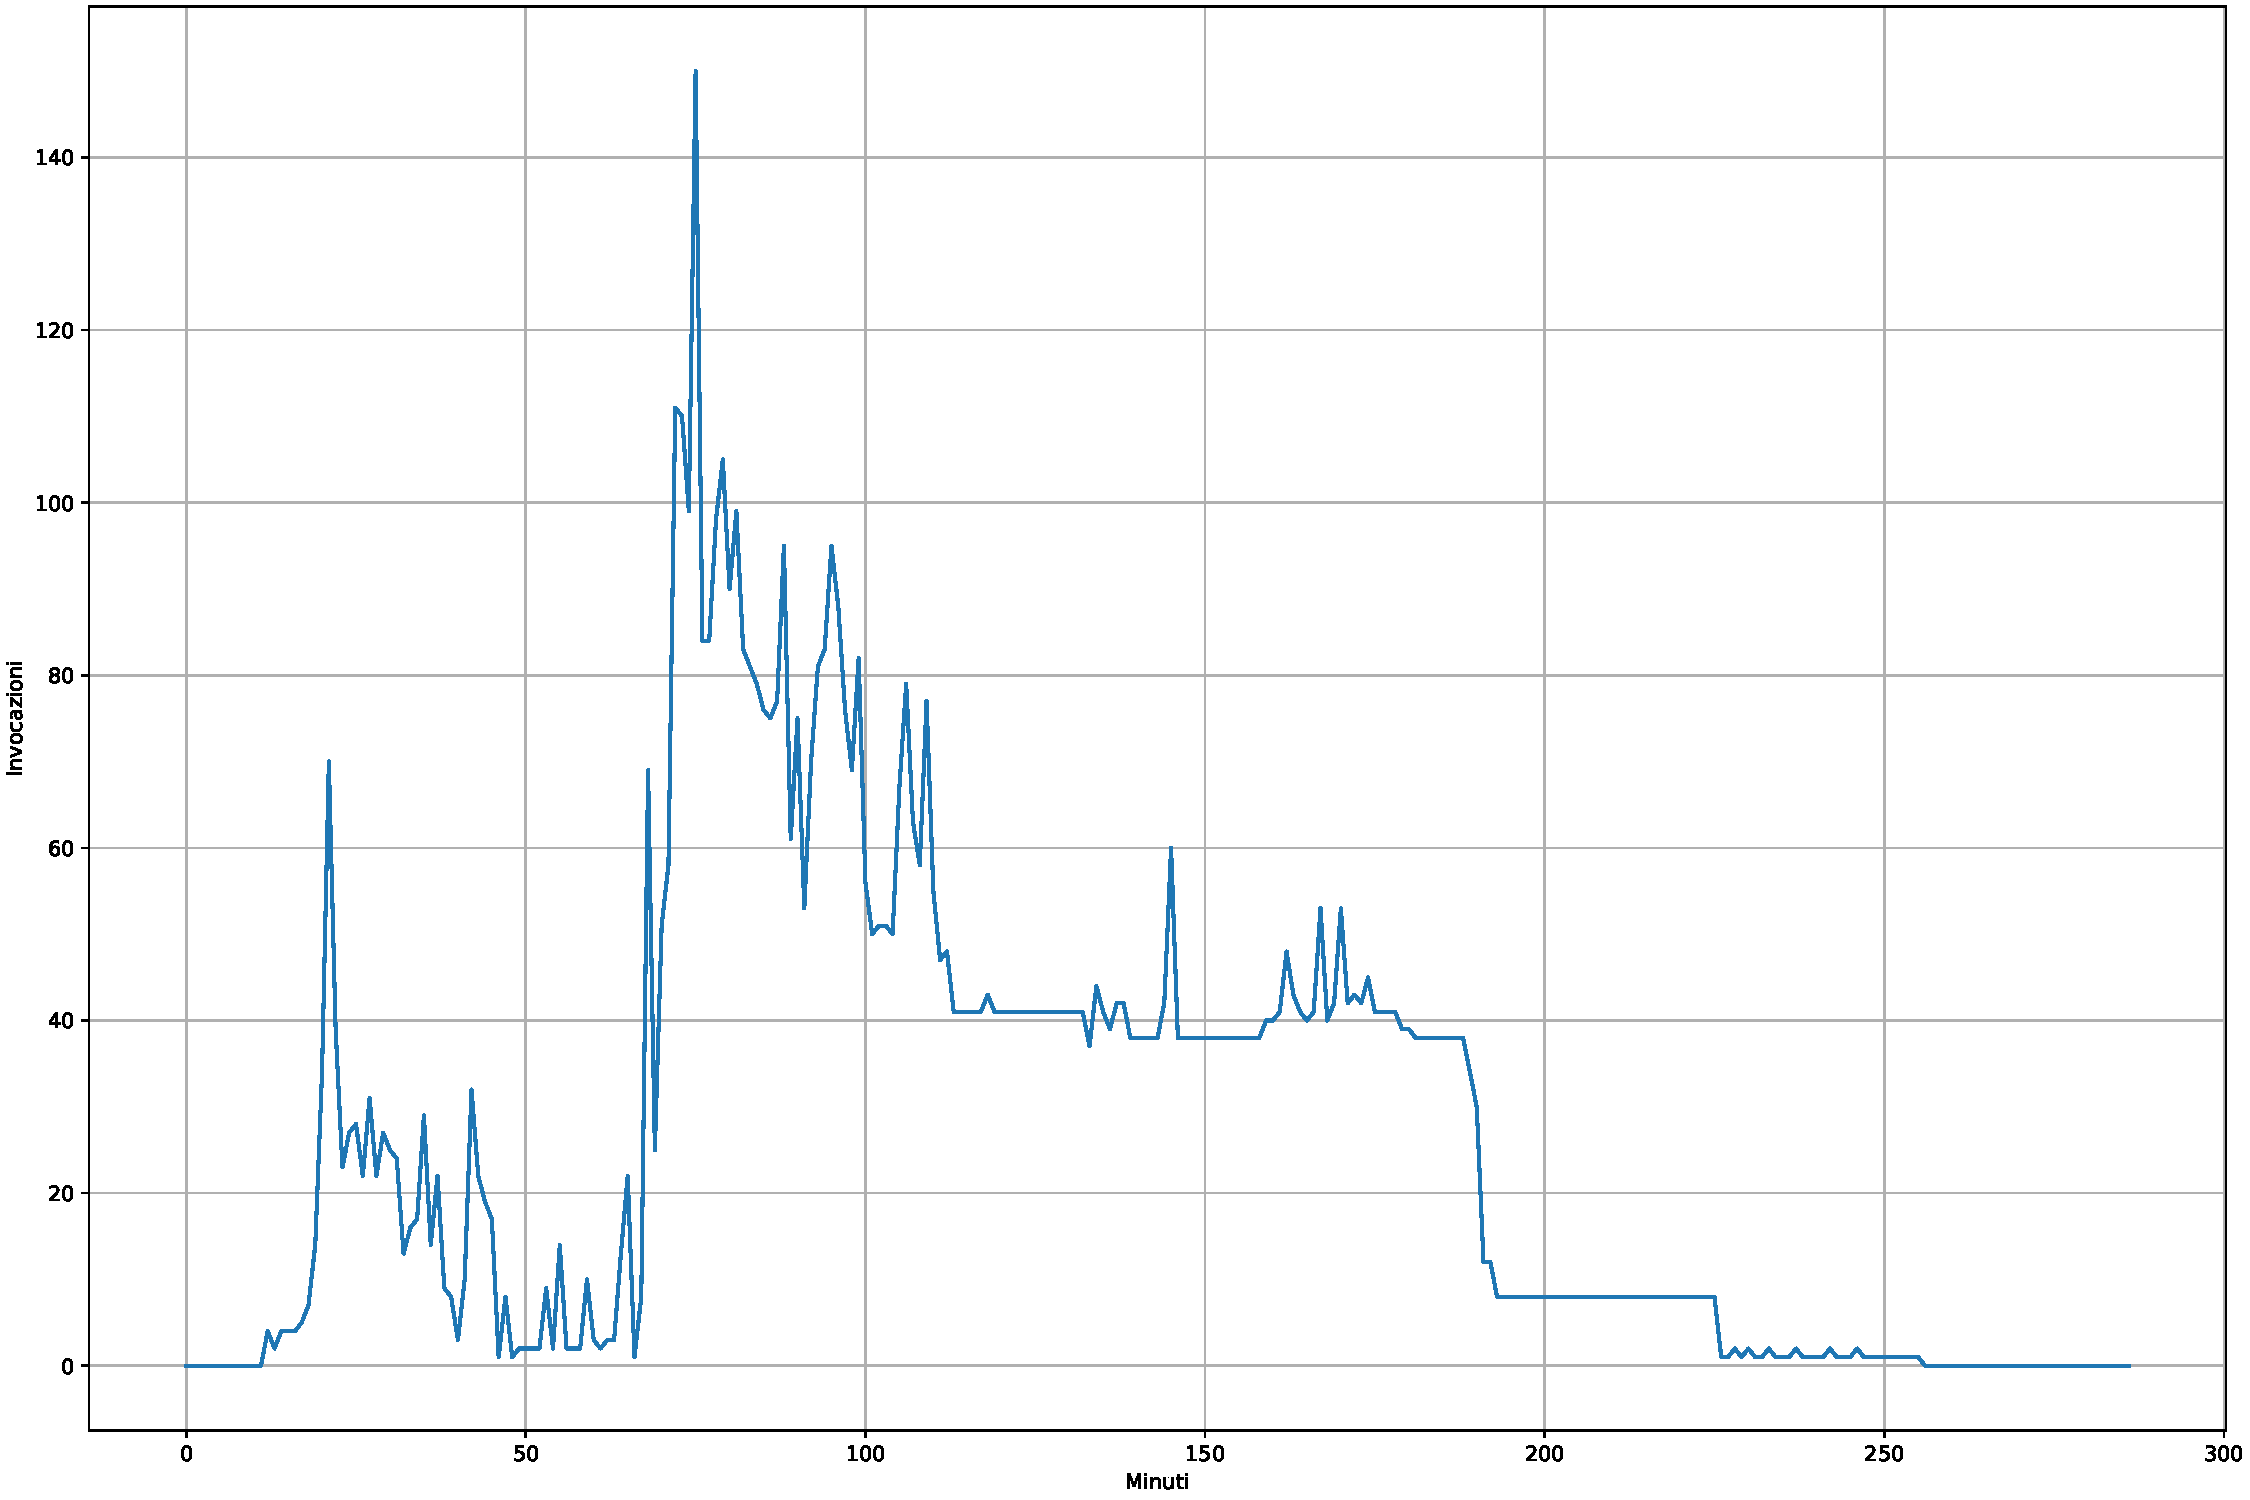
\includegraphics[width=\linewidth]{assets/5/requests_f2d88b_scaled.pdf}
        \caption{Traccia della funzione f2d88b.}
        \label{fig:5_real_traces_scaled_f2d88b}
    \end{subfigure}
    
    \caption[Tracce ridimensionate delle funzioni mostrate in \Cref{fig:5_real_traces}]{Tracce ridimensionate delle funzioni mostrate in \Cref{fig:5_real_traces}. Per ognuna sono indicati gli ultimi tre byte dell'hash di identificazione.}
    \label{fig:5_real_traces_scaled}
\end{figure}

\paragraph{Scelta delle tracce in ogni episodio.} Per lo scenario reale, l'ambiente estrae casualmente una giornata di tracce per ogni agente, e per ognuno estrae casualmente una traccia reale. L'insieme delle tracce è preso dal set di dati selezionato e ridimensionato. La distribuzione delle giornate avviene in modo esclusivo per evitare una eventuale correlazione tra le tracce in una stessa giornata, poiché più funzioni possono appartenere a una stessa applicazione. Le due estrazioni avvengono a ogni avvio dell'episodio. In aggiunta, l'intervallo delle giornate è stato suddiviso in due: un intervallo più grande di 12 giornate dedicato alla fase di addestramento, e uno più piccolo di 2 giornate dedicato alla fase di valutazione. Tale scelta è motivata per evitare di utilizzare le stesse tracce nelle due fasi.

\subsubsection{Scenari sintetici}

Lo scenario sintetico prevede la generazione dei carichi in ingresso a partire da distribuzioni o funzioni che non hanno una corrispondenza diretta con carichi reali. Sono stati definiti di seguito le due sotto-tipologie di scenari sintetici.

\paragraph{Scenario sintetico sinusoidale.} La generazione delle tracce avviene con la funzione trigonometrica del seno, con l'aggiunta di rumore generato da una distribuzione gaussiana. La sinusoide cambia periodo tre volte nel corso di un episodio, mentre rimangono costanti lo scostamento verticale intorno alla quale si sviluppa la curva e l'ampiezza delle richieste. Infine, viene applicato un rumore estratto da una distribuzione gaussiana per rendere meno prevedibile il traffico agli agenti. I periodi sono estratti casualmente da una distribuzione uniforme in $[15, 100]$, per evitare sinusoidi poco rappresentative e di difficile gestione.

L'idea alla base di questo scenario è modellare i picchi di richieste e osservare come gli agenti rispondono a tali picchi. La \Cref{fig:5_sinthetic_traces_sin_64423} mostra un esempio di tracce generate per un episodio, in cui le due sinusoidi sono parzialmente in fase. Quando l'ambiente è intorno al passo 10, si ha che entrambi gli agenti si trovano al picco della curva e non possono processare tutte le richieste in arrivo. In questo caso è inevitabile un certo numero di richieste rifiutate.

\paragraph{Scenario sintetico gaussiano.} La generazione delle tracce avviene utilizzando una distribuzione normale. La media e la deviazione standard derivano dalla media di tali valori estratti dalle tracce reali. L'idea alla base di questo scenario è costruire delle tracce con caratteristiche simili a quelle reali e osservare come gli agenti imparano a processare i carichi intorno al valore medio. La figura \Cref{fig:5_sinthetic_traces_norm_64423} mostra un esempio di generazione delle tracce per un episodio.

\begin{figure}
    \centering

    \begin{subfigure}{\textwidth}
        \centering
        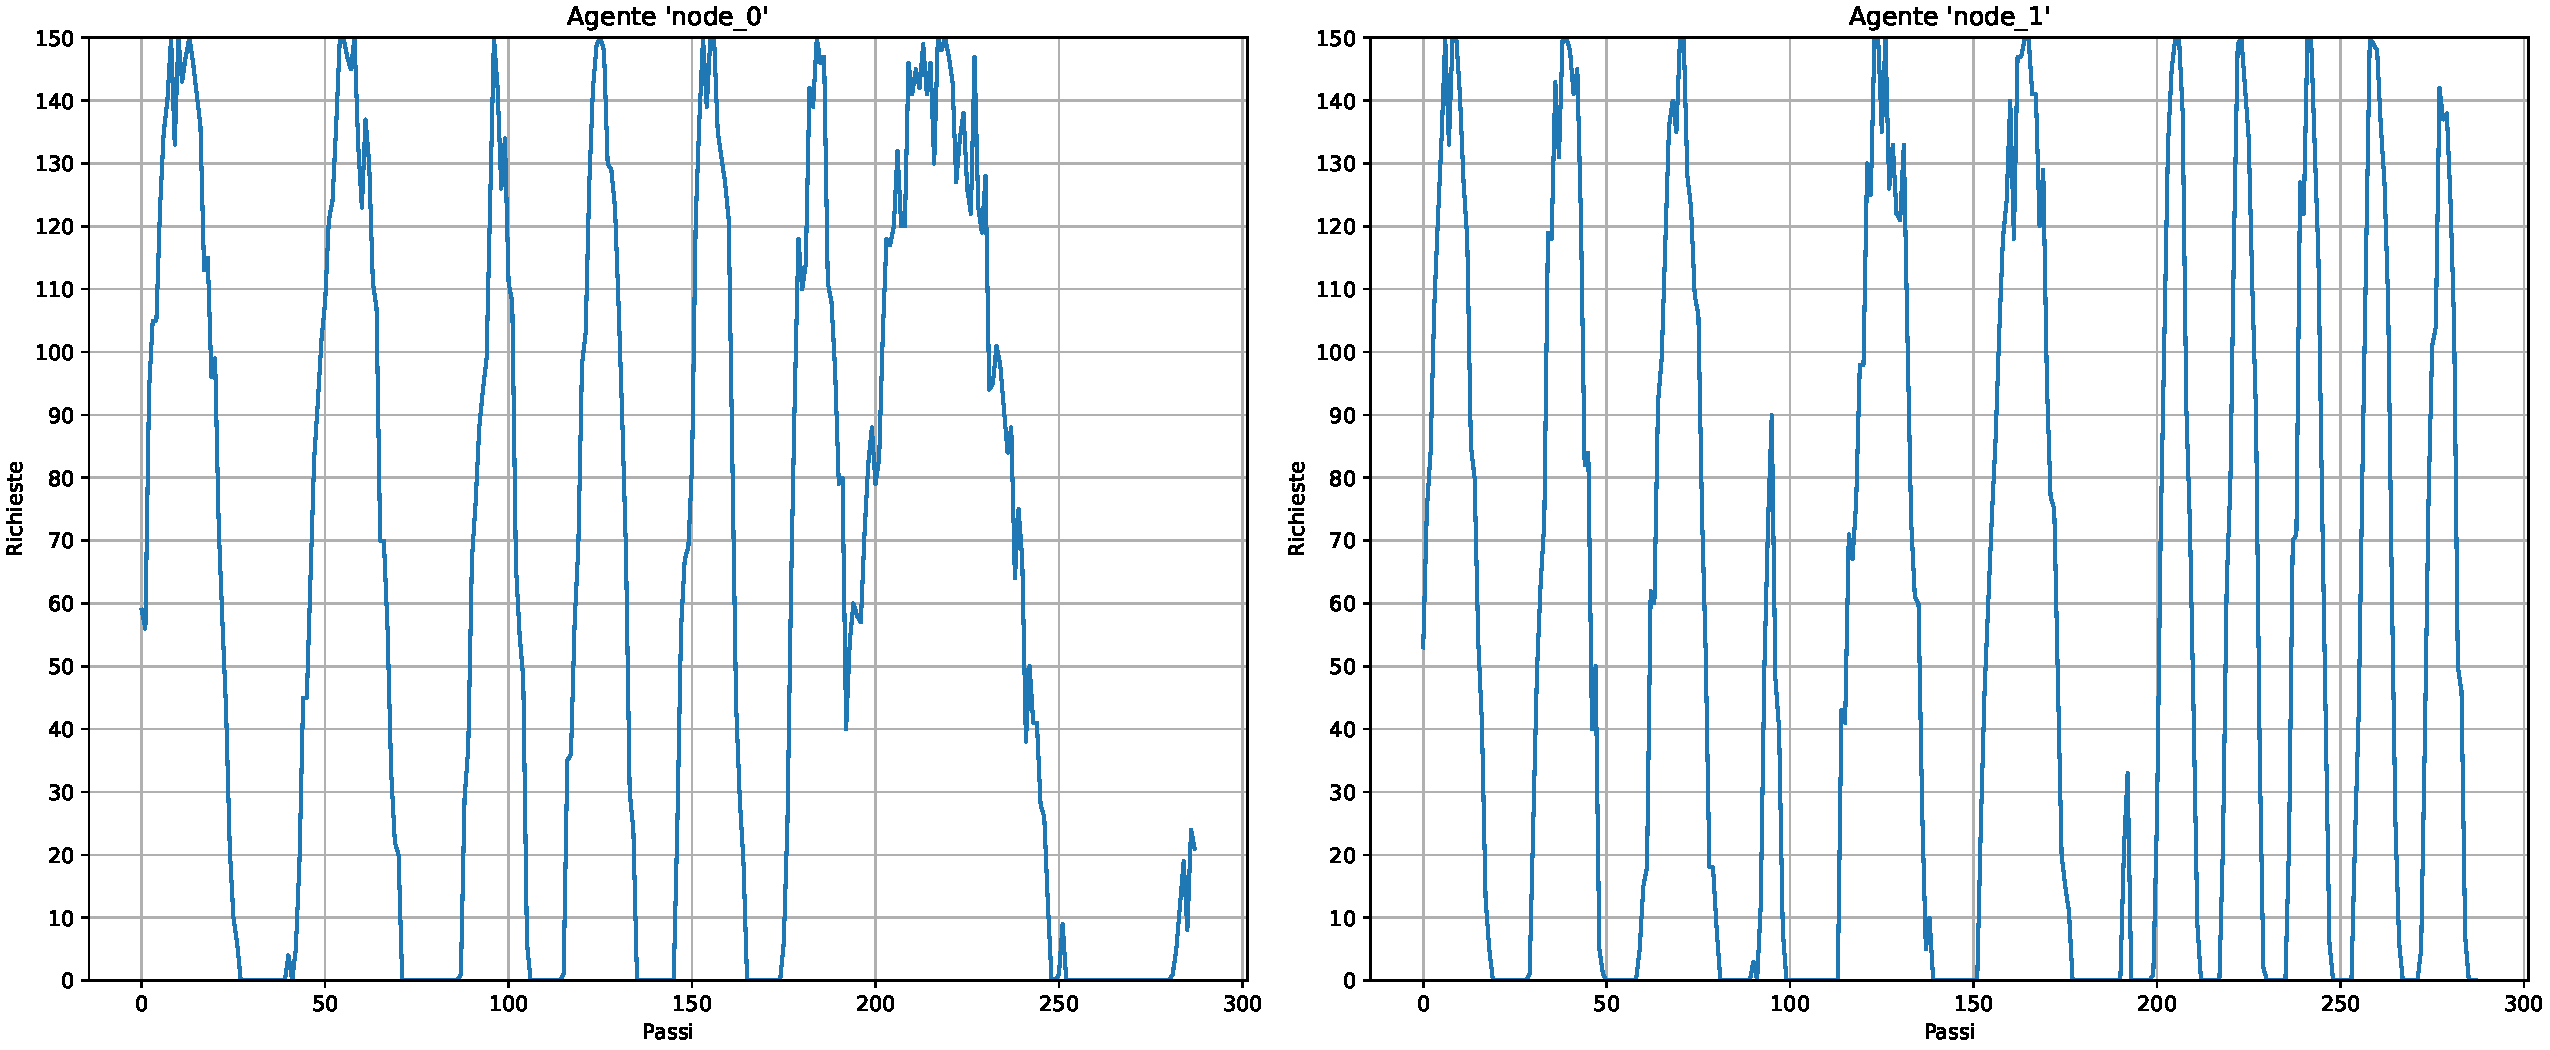
\includegraphics[width=\linewidth]{assets/5/requests_sinusoidal_64423.pdf}
        \caption{Tracce sintetiche sinusoidali. Il periodo cambia ogni circa 100 passi.}
        \label{fig:5_sinthetic_traces_sin_64423}
    \end{subfigure}

    \begin{subfigure}{\textwidth}
        \centering
        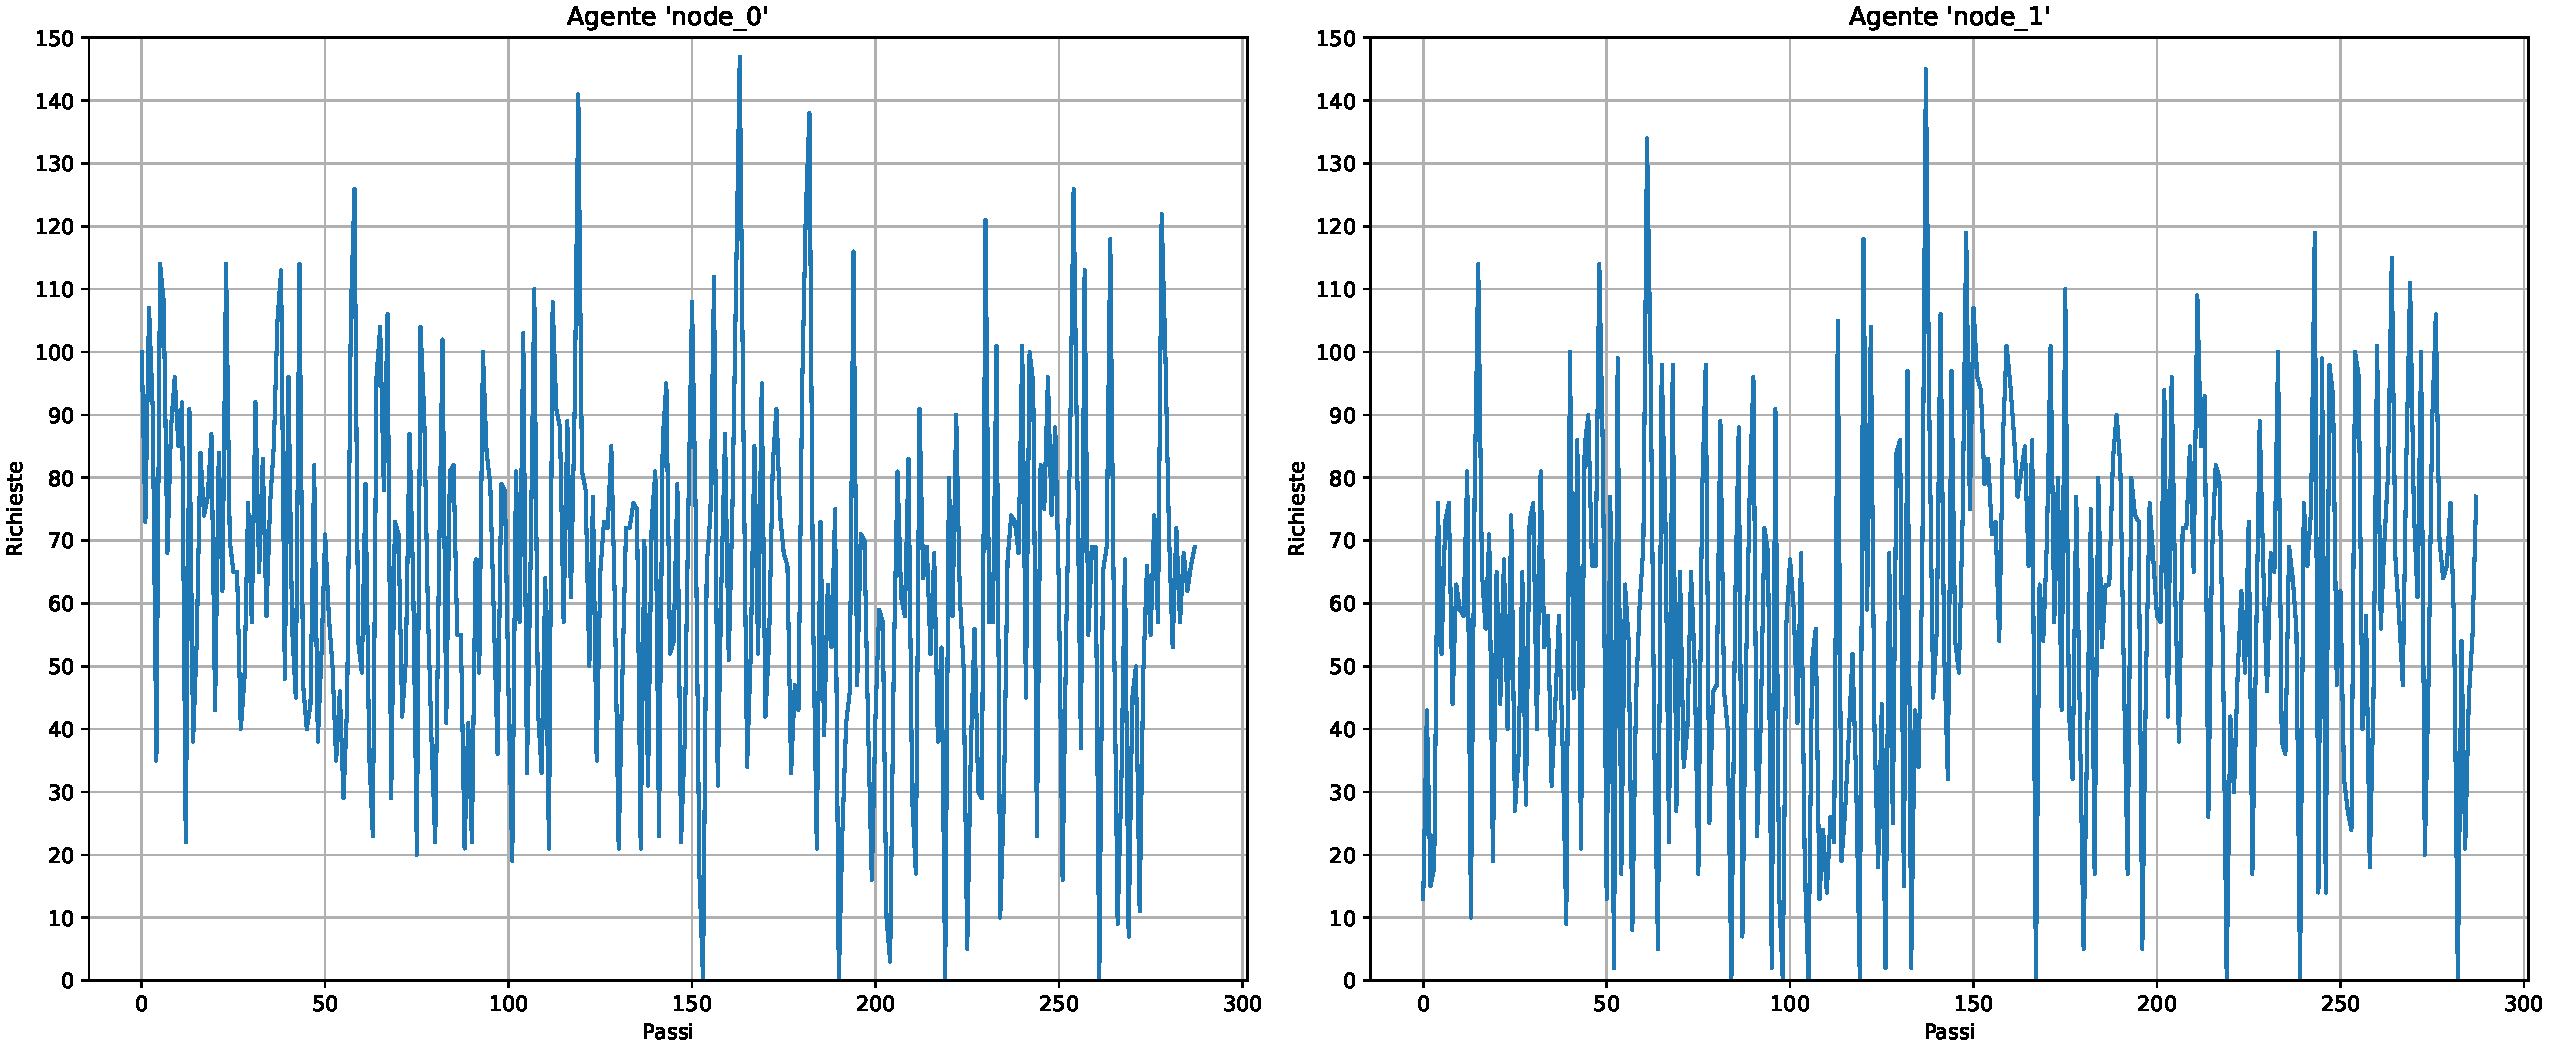
\includegraphics[width=\linewidth]{assets/5/requests_normal_64423.pdf}
        \caption{Tracce sintetiche generate da una distribuzione normale con media e deviazione standard uguale alle tracce reali.}
        \label{fig:5_sinthetic_traces_norm_64423}
    \end{subfigure}
    
    \caption[Esempi di tracce sintetiche]{Esempi di tracce sintetiche, sinusoidali e normali, generate a partire dal seed \numprint{64423}. Le tracce vengono generate all'avvio di un episodio e per tutti gli agenti dell'ambiente preso in considerazione.}
    \label{fig:5_sinthetic_traces}
\end{figure}

\subsection{Configurazione degli addestramenti}

La fase sperimentale è composta da due parti:

\begin{enumerate}
    \item \textbf{Addestramento}: ogni agente viene addestrato con le due versioni di PPO (presentate in \Cref{sec:2_rl_ppo_choices}) e tutte le possibili combinazioni di scenari e tipologia di ambienti.

    \item \textbf{Valutazione}: ogni agente addestrato viene valutato distribuendo il traffico per 50 episodi per ogni scenario.
\end{enumerate}

Ogni sessione di addestramento è stata pertanto seguita da tre sessioni di valutazione, i cui risultati sono stati registrati e categorizzati come segue:

\begin{itemize}
    \item \textbf{Risultati nello scenario di addestramento}: metriche ottenute valutando un agente con lo stesso scenario usato per l'addestramento.

    \item \textbf{Risultati negli scenari di valutazione}: metriche ottenute valutando un agente con scenari diversi da quello usato per l'addestramento.
\end{itemize}

Benché i risultati ottenuti nello scenario di addestramento siano informativi, l’attenzione principale è sui risultati di valutazione, utilizzati per valutare la capacità di generalizzazione degli algoritmi in contesti non visti in precedenza. L’obiettivo è identificare strategie che, oltre ad essere ottimizzate e validate in uno scenario di addestramento, mantengano buone prestazioni anche in scenari non direttamente esplorati durante l’addestramento.

Per ogni scenario, ambiente e algoritmo (PPO nelle due modalità multi-agente) è stato eseguito un addestramento per un totale di 18 addestramenti, seguiti da valutazioni sui scenari disponibili, per un totale di 54 valutazioni. Ogni addestramento ha la durata di 500 iterazioni, in ogni iterazione sono eseguiti 15 episodi, per un totale di \numprint{7500} episodi (o \numprint{2160000} passi di esecuzione).

La scelta delle tracce avviene tramite un generatore di numeri pseudocasuali (Random Number Generator, RNG), inizializzato con un seed. Per facilitare la riproducibilità e il confronto tra i risultati, sono stati scelti due seed, uno per la fase di addestramento e uno per la fase di valutazione.

\subsection{Algoritmi e modello}

L'algoritmo scelto per addestrare gli agenti è PPO, presentato in modo più approfondito nella \Cref{sec:2_ppo}. Tale scelta è motivata dai risultati ottenuti in \cite{Petriglia2024}, in cui risulta essere l'algoritmo che offre prestazioni migliori rispetto agli altri sia in termini di ricompensa sia in termini di generalità degli scenari provati. Come definito nella \Cref{sec:2_rl_ppo_choices}, PPO è stato usato in due configurazioni: la prima in cui ogni agente è addestrato in modo indipendente, la seconda in cui ogni agente condivide la rete neurale Critic, condividendo quindi le azioni scelte e le osservazioni di entrambi. Di seguito e nei risultati la prima configurazione viene denominata ``PPO'', mentre la seconda come ``PPO-CC'' (Centralized Critic).

La libreria RLlib implementa l'algoritmo PPO usando entrambi gli approcci per controllare l'aggiornamento della policy descritti in \Cref{sec:2_ppo}. L'implementazione è ottimizzata per velocizzare l'addestramento delle reti neurali con l'uso della GPU (possibilmente anche più di una). L'esperienza utilizzata per le iterazioni nell'ascesa del gradiente stocastica viene raccolta da più processi che giocano episodi (chiamati ``rollout worker'' in RLlib), e le sequenze di esperienze vengono mescolate prima dell'addestramento per evitare overfitting. La \Cref{fig:5_rllib_ppo_architecture} espone l'architettura di PPO implementata in RLlib.

\begin{figure}
    \centering
    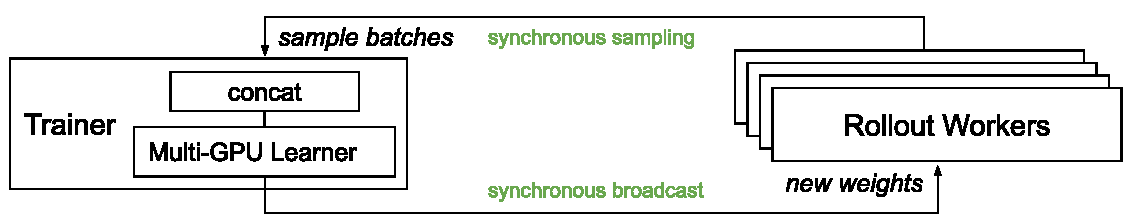
\includegraphics[width=\linewidth]{assets/5/ray_ppo_architecture.pdf}
    \caption[Architettura di PPO in RLlib]{Architettura di PPO in RLlib. Fonte: \url{https://docs.ray.io/en/releases-2.10.0/rllib/rllib-algorithms.html}}
    \label{fig:5_rllib_ppo_architecture}
\end{figure}

Negli esperimenti svolti PPO, è stato configurato con gli iperparametri predefiniti\footnote{\url{https://github.com/ray-project/ray/blob/releases/2.10.0/rllib/algorithms/ppo/ppo.py}} in RLlib, derivati dalla pubblicazione originale in \cite{Schulman2017} e ottimizzati per scenari generali. Tali iperparametri sono mostrati nella \Cref{table:5_ppo_hyperparameters}. Le implementazioni più diffuse, come quella di \cite{Raffin2021} per Stable-Baselines3\footnote{\url{https://stable-baselines3.readthedocs.io/en/master/modules/ppo.html}}, implementano solo l'approccio che usa la funzione obiettivo surrogata clipped (\Cref{sec:2_ppo_funzione_obiettivo_clipped}), mentre in RLlib entrambe sono abilitate con gli iperparametri predefiniti. Da osservazioni empiriche, combinare i due approcci garantisce prestazioni migliori rispetto ad esperimenti in cui si utilizza un solo approccio.

\begin{table}[h!]
    \centering
    \caption{Iperparametri per PPO usati negli esperimenti.}
    \begin{tabular}{l|l}
        Iperparametro & Valore \\
        \hline
        Sconto ($\gamma$) & \numprint{0.99} \\
        Parametro GAE ($\lambda$) & 1 \\
        Parametro di clip ($\epsilon$) & \numprint{0.3} \\
        Dimensione minibatch SDG & 128 \\
        Iterazioni SDG & 30 \\
        Coefficiente di entropia & 0 \\
        Tasso di apprendimento & $5 \times 10^{-5}$ \\
        Coefficiente KL ($\beta$) & \numprint{0.2} \\
        Target KL $d_\textnormal{targ}$ & \numprint{0.01} \\
        Coefficiente VF & 1 \\
        Parametro di clip per VF & 10 \\
    \end{tabular}
    \label{table:5_ppo_hyperparameters}
\end{table}

Nonostante l'implementazione di PPO in RLlib contenga una differenza nell'aggiornamento del coefficiente KL\footnote{\url{https://github.com/ray-project/ray/issues/15698}} rispetto alla versione originale, gli effetti sono trascurabili perché l'algoritmo automaticamente corregge il valore, come indicato in \cite{Schulman2017}. Lo stesso vale per il valore iniziale di $\beta$.

Come per l'implementazione in Stable-Baselines3, anche in quella di RLlib viene utilizzata la Generalized Advantage Estimation (GAE) per calcolare il gradiente della policy, introdotta per la prima volta in \cite{Schulman2015}.

\paragraph{Modello.} PPO utilizza il framework actor-critic, in cui ci sono due reti neurali, una rete actor (la rete policy) e una rete critic (la funzione di valore). Per gli esperimenti è stato scelto di utilizzare il modello di rete completamente connesso predefinito in RLlib, con due strati nascosti da 256 nodi ciascuna e Tanh come funzione di attivazione anche per l'ultimo strato di output. RLlib gestisce automaticamente il primo stato di input e l'ultimo strato di output in base alle dimensioni dello spazio delle osservazioni e delle azioni.

\subsection{Metriche di valutazione}

Per ogni esperimento, sia di addestramento sia di valutazione, sono stati registrati dati relativi all'esecuzione degli episodi, compreso lo stato dell'ambiente, le azioni e le ricompense ottenute a ogni passo. Da questi dati è possibile calcolare una serie di metriche per valutare le prestazioni degli agenti. Nel caso di studio sono state selezionate due metriche principali:

\begin{itemize}
    \item \textbf{Numero di richieste processate totali}: calcolata per episodio, è la metrica più importante perché indica se l'agente (o gli agenti se si considerano tutti gli agenti) ha distribuito in maniera ottimale il carico in ingresso. È una metrica da massimizzare.

    \item \textbf{Ricompensa totale}: calcolata per episodio, indica se le azioni scelte da un agente (o più agenti) sono state ottimali secondo la funzione di ricompensa. È una metrica da massimizzare.
\end{itemize}

A partire da queste metriche singole per ogni agente, sono state poi considerate metriche derivate tra le quali la deviazione standard e la media sia per il singolo agente sia per la somma di entrambi gli agenti. Nelle sottosezioni seguenti sono approfondite le due metriche selezionate.

\subsubsection{Numero di richieste processate totali}

Il numero di richieste processate totali è la la somma delle richieste processate localmente e inoltrate senza essere state rifiutate per ogni passo per ogni agente agente.

Formalmente, per ogni agente è possibile calcolare il numero di richieste processate per un episodio come

\begin{equation}
    P_n \coloneqq \sum_{t=1}^{288} \left( r^\textnormal{L}_t - e^\textnormal{L}_t + r^\textnormal{F}_t - e^\textnormal{FR}_t \right) \quad \forall n \in \mathcal{N},
\end{equation}

in cui i termini definiti nelle \Cref{sec:4_modellazione_elementi,sec:4_funzione_ricompensa} fanno riferimento al $t$-esimo passo dell'episodio per l'agente preso in considerazione. In caso di agenti che non possono inoltrare, i termini $r^\textnormal{F}_t$ e $e^\textnormal{FR}_t$ sono omessi. Il numero di richieste processate per l'intero ambiente è quindi la somma dei singoli contributi

\begin{equation}
    P \coloneqq \sum_{n}^{\mathcal{N}} P_n.
\end{equation}

La somma $P$ è la metrica considerata per confrontare le prestazioni tra esperimenti con ambienti, algoritmi e scenari diversi. Più il valore è alto e più gli agenti sono stati in grado di processare le richieste, minimizzando le richieste rifiutate.

\paragraph{} Data la natura degli esperimenti in ambiente simulato e semplificato (capacità della coda locale costante e uguale per tutti gli agenti e con gli slot che si liberano a ogni passo), è possibile definire il massimo numero di richieste processabili in un passo $t$ per entrambi gli agenti $P^\textnormal{MAX}_t$ come

\begin{equation}
    P^\textnormal{MAX}_t \coloneqq \begin{dcases}
        R^\textnormal{IN}_t & \textnormal{se } R^\textnormal{IN}_t \le q^\textnormal{MAX} \cdot |\mathcal{N}| \\
        q^\textnormal{MAX} \cdot |\mathcal{N}| & \textnormal{altrimenti}
    \end{dcases}.
\end{equation}

A partire da $P^\textnormal{MAX}_t$ si definisce il massimo numero di richieste processabili per l'intero episodio $P^\textnormal{MAX}$, cioè l'ottimo desiderabile, come

\begin{equation}
    P^\textnormal{MAX} \coloneqq \sum_{t=1}^{288} P^\textnormal{MAX}_t
\end{equation}

Ad ogni passo, gli agenti possono processare un massimo di richieste che dipende dalla capacità della coda: se in un passo le richieste in arrivo eccedono tale capacità, l'eccesso verrà inevitabilmente rifiutato. La pura somma delle richieste in arrivo per entrambi gli agenti $R^\textnormal{IN}$ non è un limite che si può considerare, poiché, in base a come le richieste sono distribuite in ingresso, il limite $P^\textnormal{MAX}$ può variare sensibilmente. Ne consegue che

\begin{equation*}
    P^\textnormal{MAX} \le R^\textnormal{IN}.
\end{equation*}

Considerando ad esempio le tracce mostrate in \Cref{fig:5_sinthetic_traces}, sono stati calcolati nella \Cref{table:5_total_input_requests_example} i valori di $P^\textnormal{MAX}$ e $R^\textnormal{IN}$. Nei momenti di picco delle tracce sinusoidali, il numero di richieste in ingresso eccede di molto le capacità delle code degli agenti; pertanto, le richieste devono essere rifiutate, situazione che si aggrava quando le sinusoidi sono in fase. Questo non avviene per le tracce gaussiane, dal momento che la media della distribuzione è inferiore alla capacità della coda.

\begin{table}[h!]
    \centering
    \caption{Valori di $P^\textnormal{MAX}$ e $R^\textnormal{IN}$ per le tracce in \Cref{fig:5_sinthetic_traces}.}
    \begin{tabular}{l|l|l}
        Tipologia traccia & $P^\textnormal{MAX}$ & $R^\textnormal{IN}$\\
        \hline
        Sinusoidale & \numprint{31698} & \numprint{34195} \\
        Normale & \numprint{35215} & \numprint{35375} \\
    \end{tabular}
    \label{table:5_total_input_requests_example}
\end{table}

La \Cref{fig:5_processable_requests_synthetic} mostra la somma delle tracce in \Cref{fig:5_sinthetic_traces}, con l'area della parte colorata in verde che corrisponde a $P^\textnormal{MAX}$, mentre l'area della parte colorata in rosso è $R^\textnormal{IN} - P^\textnormal{MAX}$, cioè le richieste necessariamente da rifiutare.

\begin{figure}
    \centering
    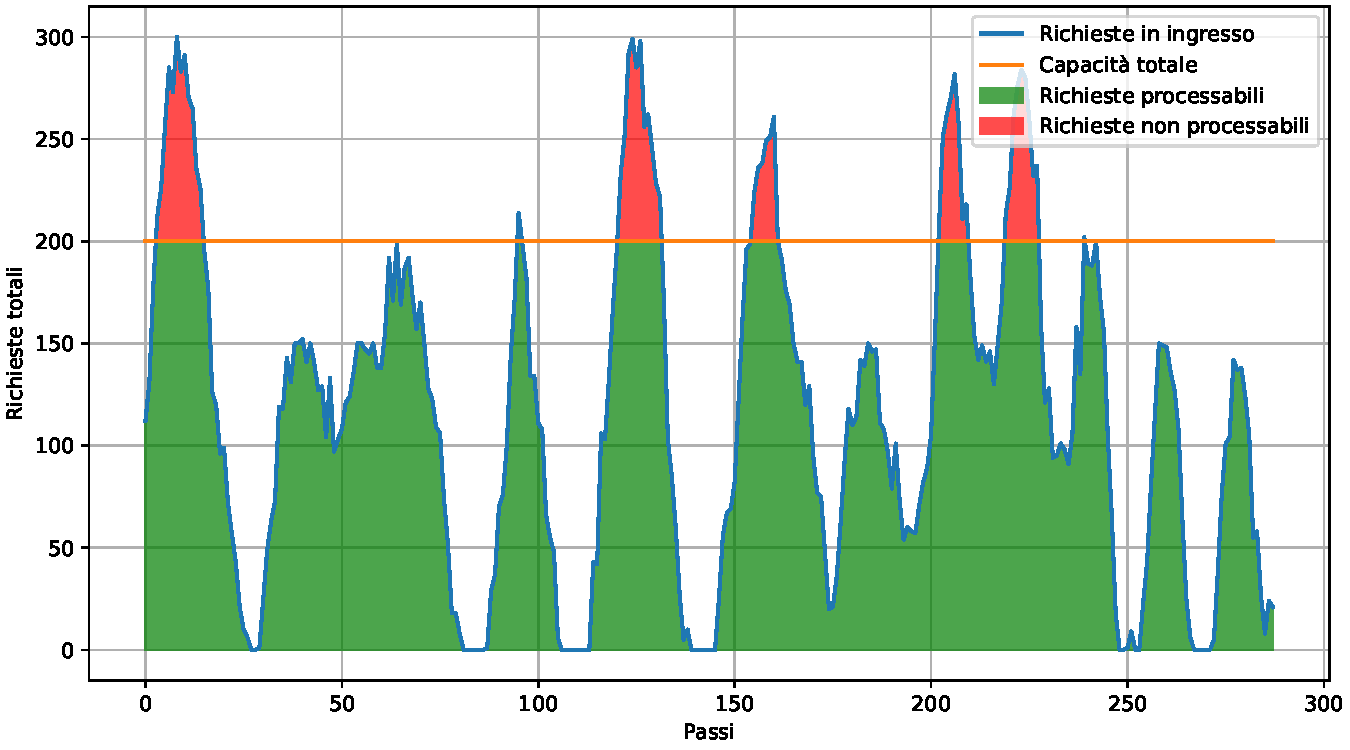
\includegraphics[width=\linewidth]{assets/5/processable_requests_sinusoidal_64423.pdf}
    \caption{Somma delle tracce in \Cref{fig:5_sinthetic_traces}. L'area in verde corrisponde a $P^\textnormal{MAX}$.}
    \label{fig:5_processable_requests_synthetic}
\end{figure}

\subsubsection{Ricompensa totale}
\label{sec:5_total_reward}

La ricompensa di un episodio è la somma delle singole ricompense ottenute in ogni passo per uno o più agenti. Per come le funzioni sono state definite, un agente può ottenere al massimo 288 come punteggio limite superiore di ricompensa cumulative:

\begin{itemize}
    \item Nel caso della \textbf{funzione senza inoltro} $\mathcal{R}$, questo avviene quando l'agente elabora tutte le richieste localmente e rifiuta solamente quelle che eccedono la dimensione della coda locale.

    \item Nel caso della \textbf{funzione con inoltro} $\mathcal{R}^\textnormal{FW}$, questo avviene quando l'agente elabora tutte le richieste localmente e inoltra le richieste che eccedono gli slot disponibili per la coda locale. Delle richieste inoltrate, nessuna deve essere stata rifiutata dall'altro agente.
\end{itemize}

\paragraph{Rifiuto inevitabile per $\mathcal{R}^\textnormal{FW}$.} Considerando la funzione con inoltro, il caso citato nell'elenco può avvenire solo in scenari con tracce senza picchi di richieste e con richieste equamente distribuite per la durata dell'episodio. In condizioni normali il rifiuto è inevitabile con tracce con picchi sovrapponibili tra i due agenti, perché entrambi gli agenti esauriscono gli slot disponibili della coda locale. Ne consegue che l'agente otterrà un punteggio inferiore al massimo teorico.

Una caso di esempio è riportato nell'\Cref{eq:5_reward_fw_non_optimal}, in cui l'agente distribuire 103 richieste in ingresso con capacità della coda fissa a 100. Le prime 100 richieste sono processate localmente, utilizzando tutti gli slot disponibili, mentre delle 3 richieste rimanenti, 2 le rifiuta e 1 la inoltra, con quest'ultima che non viene rifiutata dall'altro agente. Poiché l'unica richiesta inoltrata non è stata rifiutata, l'azione non è considerata ottimale dal punto di vista della funzione di ricompensa. Infatti, non conoscendo il numero di slot disponibili dell'agente vicino, ma vedendo solo che l'unica richiesta inoltrata non è stata rifiutata, essa ipotizza che anche le altre due richieste avrebbero potuto essere inoltrate. Nell'\Cref{eq:5_reward_fw_optimal} invece l'agente gestisce in modo diverso le 3 richieste rimanenti: ne rifiuta una e inoltra due. Dal momento che una delle due richieste inoltrate viene rifiutata, la scelta di rifiutare una richiesta viene valutata positivamente, in quanto inevitabile.

\begin{equation}\label{eq:5_reward_fw_non_optimal}
    \begin{split}
        \mathcal{R}^\textnormal{FW}(r^\textnormal{L} = 100, r^\textnormal{F} = \mathbf{1}, r^\textnormal{R} = \mathbf{2}, e^\textnormal{L} = 0, e^\textnormal{FW} = \mathbf{0}, \\ q^\textnormal{FREE} = 0, q^\textnormal{MAX} = 100) \approx 0.98
    \end{split}
\end{equation}
\begin{equation}\label{eq:5_reward_fw_optimal}
    \begin{split}
        \mathcal{R}^\textnormal{FW}(r^\textnormal{L} = 100, r^\textnormal{F} = \mathbf{2}, r^\textnormal{R} = \mathbf{1}, e^\textnormal{L} = 0, e^\textnormal{FW} = \mathbf{1}, \\ q^\textnormal{FREE} = 0, q^\textnormal{MAX} = 100) \approx 0.99 
    \end{split}
\end{equation}

\paragraph{Comparazione di $\mathcal{R}$ e $\mathcal{R}^\textnormal{FW}$.} Gli esperimenti con ambienti che coinvolgono agenti che usano funzioni di ricompensa differenti non sono direttamente comparabili in termini di ricompensa, perché il calcolo per le due funzioni segue logiche diverse. Per questo motivo nella \Cref{sec:5_risultati} sono confrontate le ricompense solo per agenti che usano la stessa funzione di ricompensa.

\section{Risultati preliminari}
\label{sec:5_risultati}

In questa sezione vengono presentati i risultati degli esperimenti, svolti secondo le modalità descritte nella precedente sezione.

\paragraph{Ricompensa media totale.} In primo luogo sono riportate, in \Cref{fig:5_results_reward}, le ricompense medie in fase di valutazione degli agenti addestrati nei tre ambienti con i due approcci di PPO. Considerando un ambiente, i valori della ricompensa per una singola coppia (scenario, algoritmo) sono mediati sulle tre valutazioni svolte, una per ogni scenario, e su 50 episodi considerati in ogni valutazione. Le ricompense dei due agenti sono sommate, in modo da ottenere un unico valore. In figura è anche riportata la ricompensa massima assoluta che i due agenti possono ottenere, calcolata come 288 (il numero di passi) per il numero di agenti dell'ambiente.

Come riportato nella \Cref{sec:5_total_reward}, si possono confrontare le ricompense solo tra esperimenti con lo stesso ambiente. Inoltre, nell'ambiente asimmetrico poiché i due agenti ricevono la ricompensa da due funzioni diverse, una ricompensa maggiore per una non identifica automaticamente un agente migliore dell'altro. Tuttavia la ricompensa è comunque uno strumento utile per osservare se gli agenti imparano.

\begin{figure}
    \centering

    \begin{subfigure}{.65\textwidth}
        \centering
        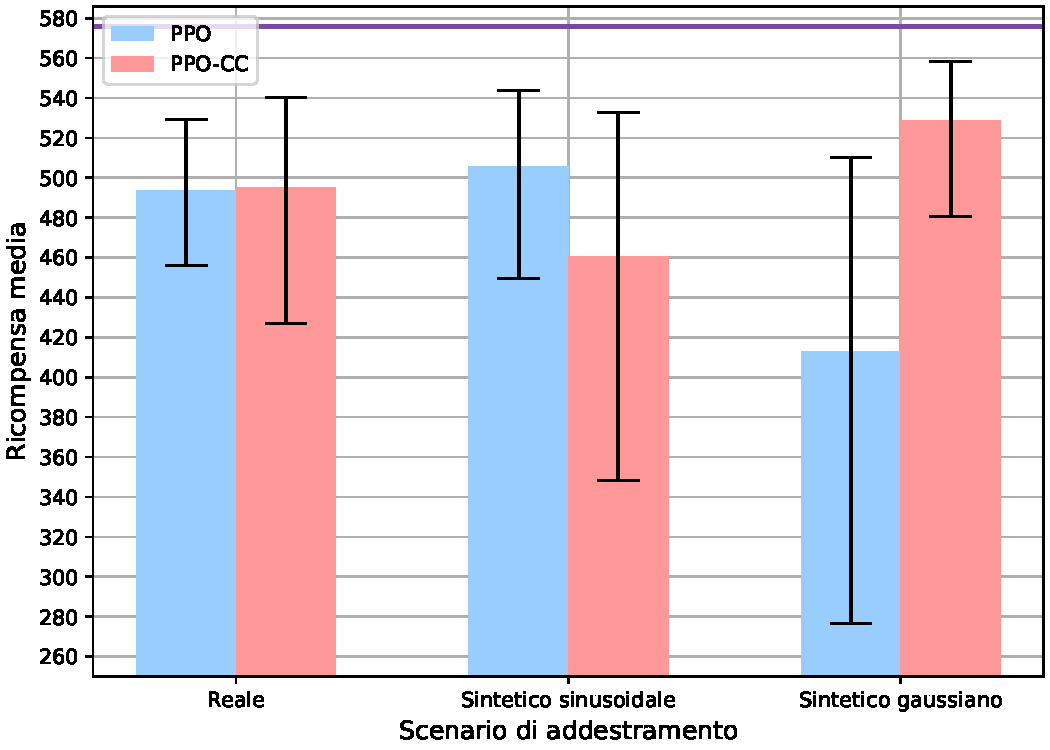
\includegraphics[width=\linewidth]{assets/5/results/eval_BASE_summary_reward.pdf}
        \caption{Ambiente ``BASE''.}
    \end{subfigure}
    
    \begin{subfigure}{.65\textwidth}
        \centering
        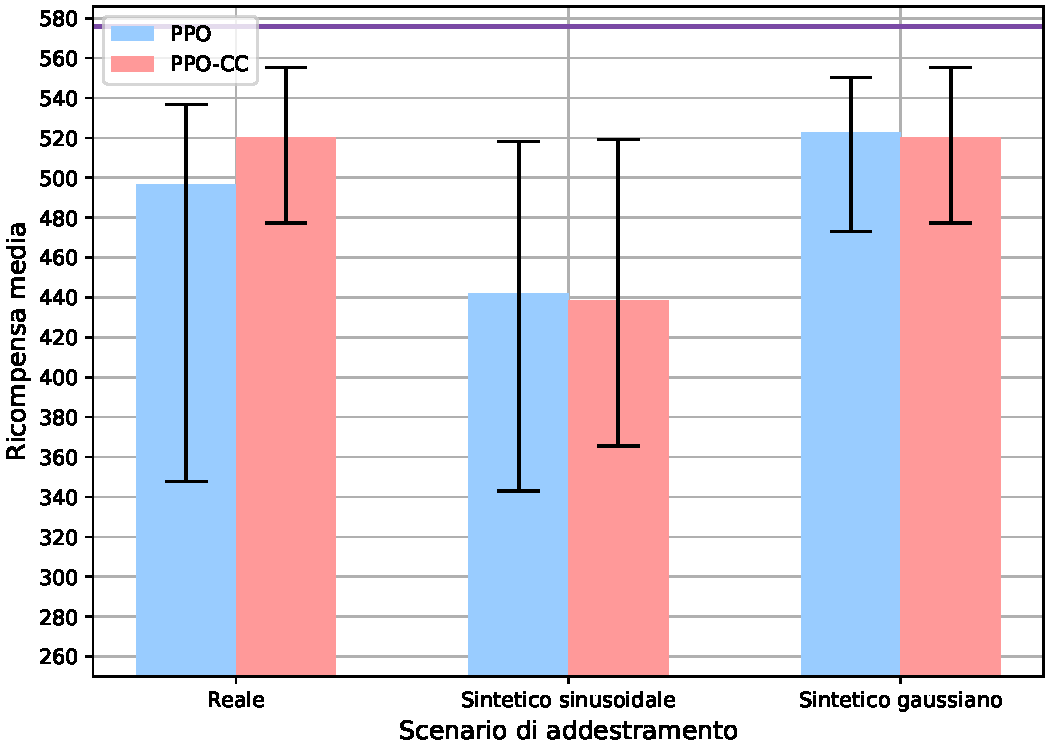
\includegraphics[width=\linewidth]{assets/5/results/eval_ASYM_summary_reward.pdf}
        \caption{Ambiente ``ASYM''.}
    \end{subfigure}
    
    \begin{subfigure}{.65\textwidth}
        \centering
        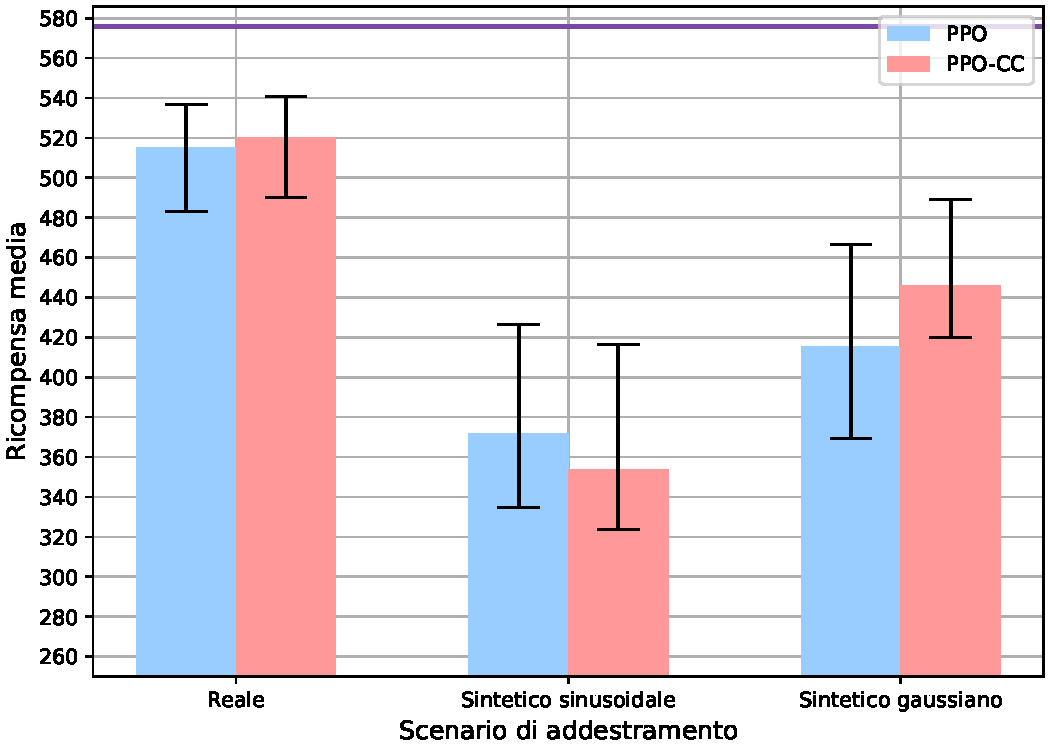
\includegraphics[width=\linewidth]{assets/5/results/eval_SYM_summary_reward.pdf}
        \caption{Ambiente ``SYM''.}
    \end{subfigure}
    
    \caption[Ricompensa media nelle valutazioni]{Ricompensa media su tutte le valutazioni con valori di minimo e massimo (in nero). La linea orizzontale indica la massima ricompensa ottenibile per episodio.}
    \label{fig:5_results_reward}
\end{figure}

Per l'ambiente simmetrico senza inoltro lo scenario reale risulta essere il migliore, considerando la ricompensa media per entrambi gli algoritmi. Lo scenario gaussiano con PPO ottiene un valore medio della ricompensa decisamente inferiore rispetto agli altri esperimenti, oltre ad avere una grande variabilità.

% La \Cref{fig:5_eval_base_train_normal_reward} mostra in dettaglio le valutazioni di questo esperimento, mediate sui 50 episodi svolti. 

% Nonostante gli agenti siano addestrati sullo scenario gaussiano, si ottiene una ricompensa inferiore rispetto allo scenario sinusoidale. C'è una forte variabilità per lo scenario gaussiano e reale con PPO, rispetto alla controparte PPO-CC oppure allo scenario sinusoidale. In questi scenari gli agenti non riescono ad imparare a processare in modo ottimale le richieste.

% \begin{figure}
%     \centering
%     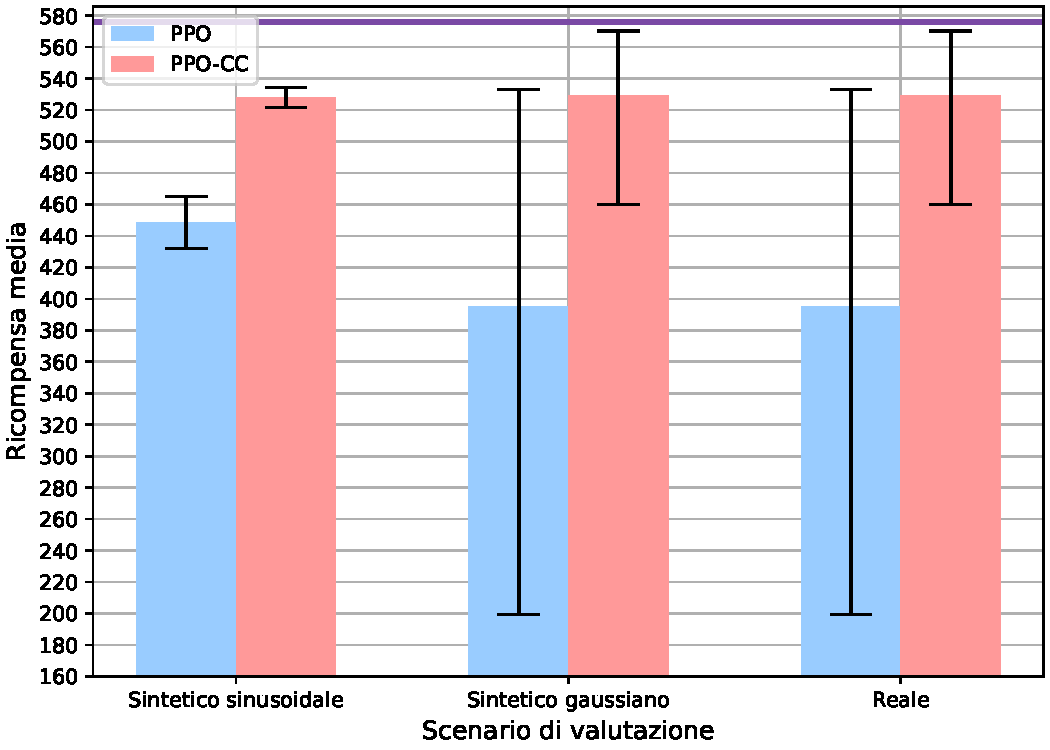
\includegraphics[width=.6\linewidth]{assets/5/results/eval_BASE_train_synthetic-normal_summary_reward.pdf}
%     \caption[Ricompensa media per l'ambiente BASE nello scenario gaussiano]{Ricompensa media per l'ambiente BASE addestrato nello scenario gaussiano e valutato sui tre scenari. In nero sono i valori di minimo e massimo. La linea orizzontale indica la massima ricompensa ottenibile per episodio.}
%     \label{fig:5_eval_base_train_normal_reward}
% \end{figure}

Per l'ambiente asimmetrico, lo scenario sinusoidale risulta essere il più difficile, mentre il gaussiano il più semplice seguito dal reale. L'ambiente simmetrico con inoltro conferma questa tendenza, con un decisa differenza tra i due scenari sintetici e lo scenario reale.

In \Cref{fig:5_train_real_reward} è mostrata la ricompensa media per iterazione durante l'addestramento degli agenti in ambiente simmetrico con inoltro e scenario reale. Si può osservare come, nonostante la versione con PPO-CC parta peggio rispetto a PPO, sulle iterazioni più lunghe le due versioni si comparano e PPO-CC supera PPO. Questo si conferma osservando il risultato aggregato \Cref{fig:5_results_reward}: con l'unica eccezione dello scenario sintetico sinusoidale, PPO-CC è molto vicino a PPO oppure migliore.

\begin{figure}
    \centering
    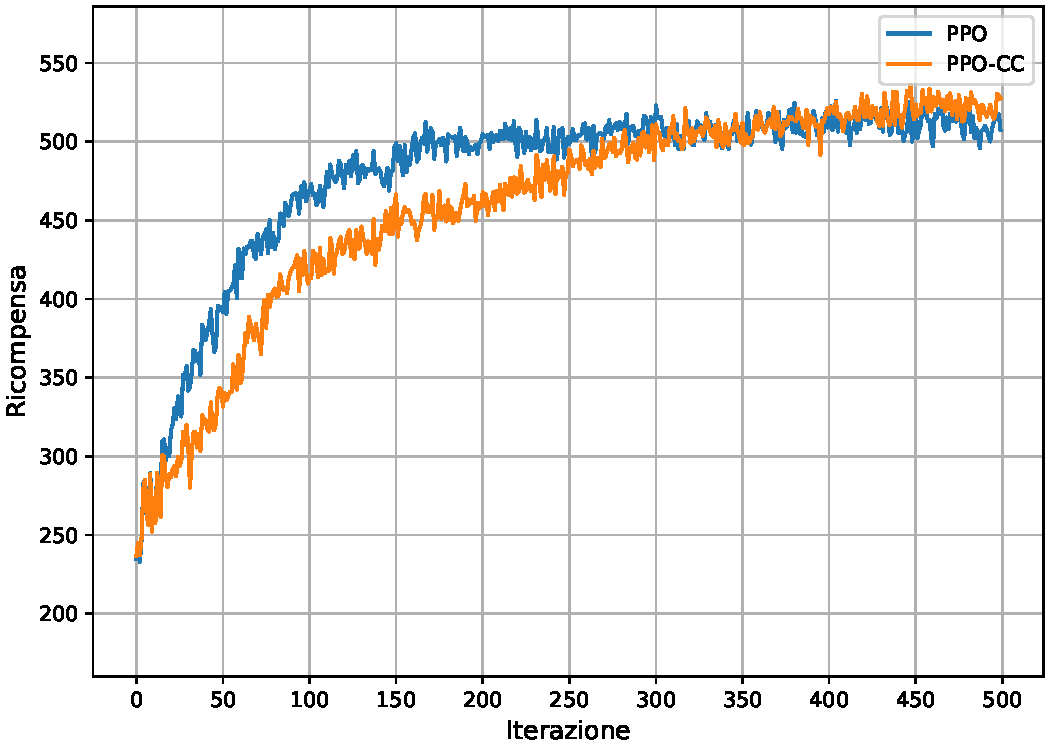
\includegraphics[width=.7\linewidth]{assets/5/results/train_real_summary_reward.pdf}
    \caption{Ricompensa media per iterazione ottenuta durante l'addestramento degli agenti con l'ambiente SYM su scenario reale.}
    \label{fig:5_train_real_reward}
\end{figure}

\paragraph{Numero di richieste processate.} In \Cref{fig:5_results_requests} sono mostrate le percentuali medie di richieste processate sul numero di richieste processabili per episodio, per ogni combinazione di scenario, ambiente e algoritmo. Come per la \Cref{fig:5_results_reward}, i valori sono medi sulle valutazioni per un singolo esperimento e sommati per i due agenti.

\begin{figure}
    \centering

    \begin{subfigure}{.8\textwidth}
        \centering
        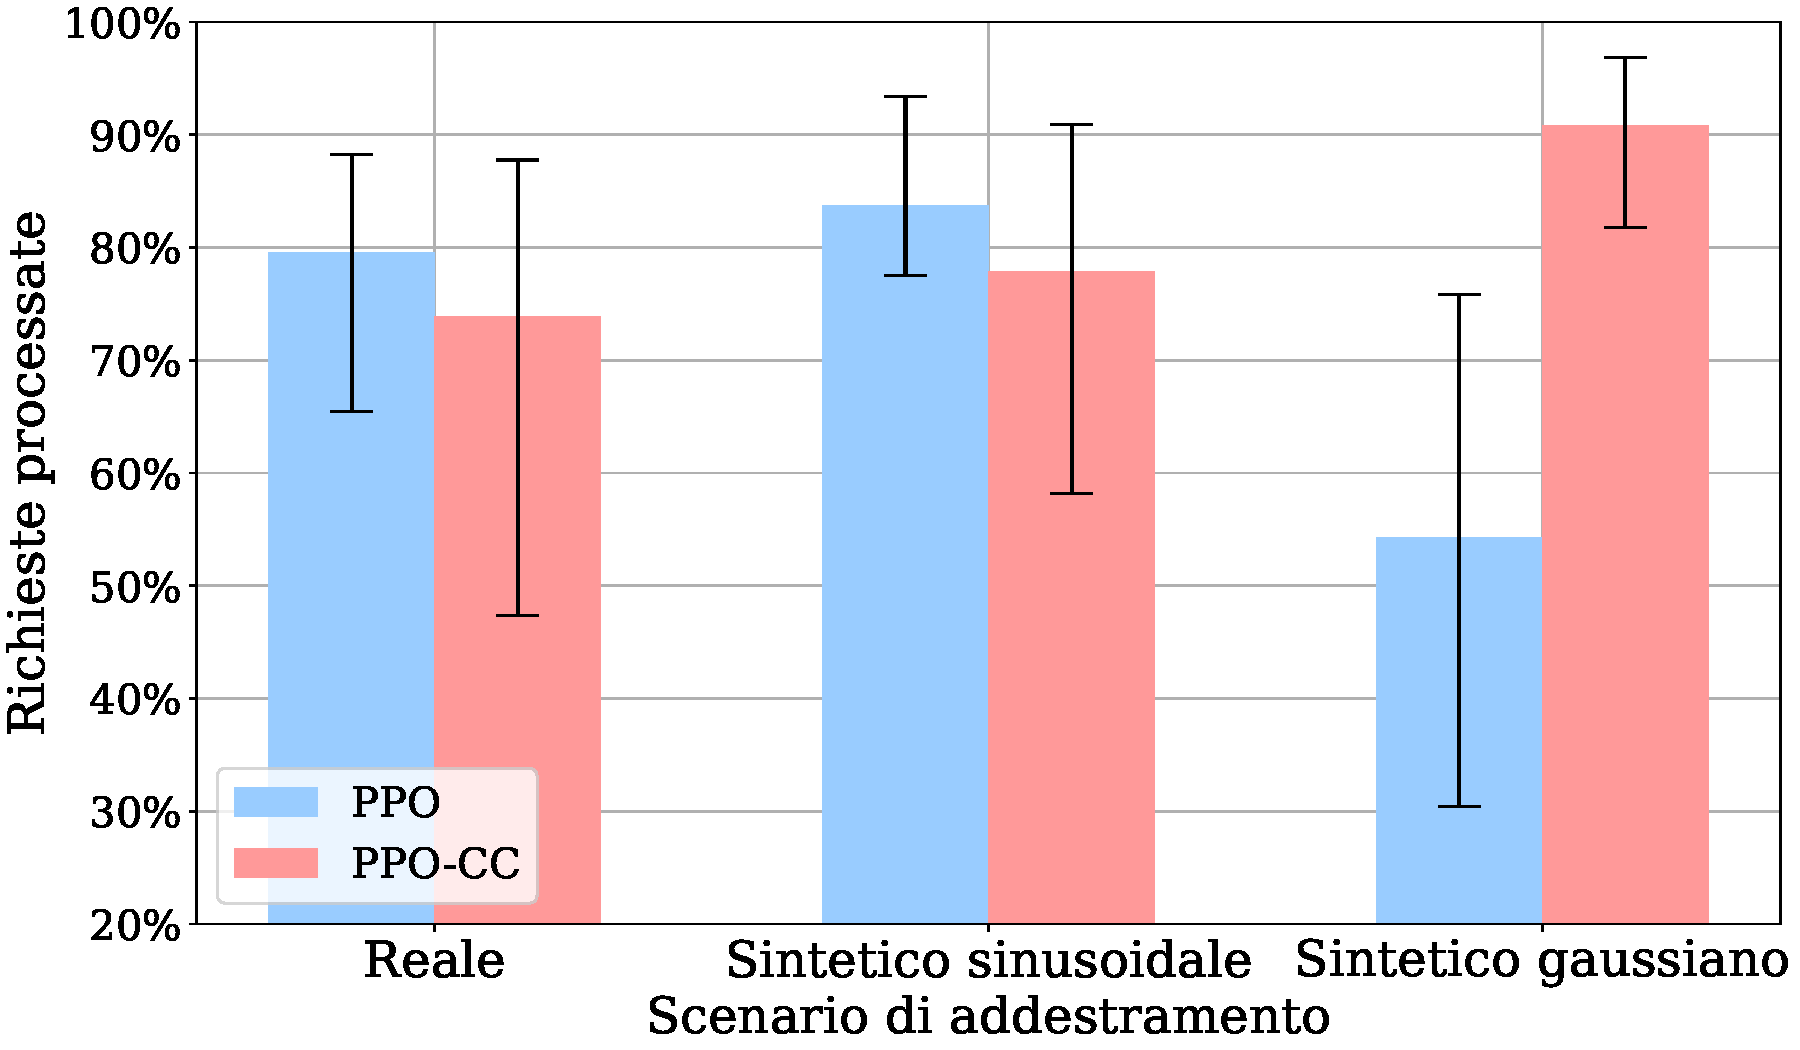
\includegraphics[width=\linewidth]{assets/5/results/eval_BASE_summary_processed_requests.pdf}
        \caption{Ambiente ``BASE''.}
    \end{subfigure}
    
    \begin{subfigure}{.8\textwidth}
        \centering
        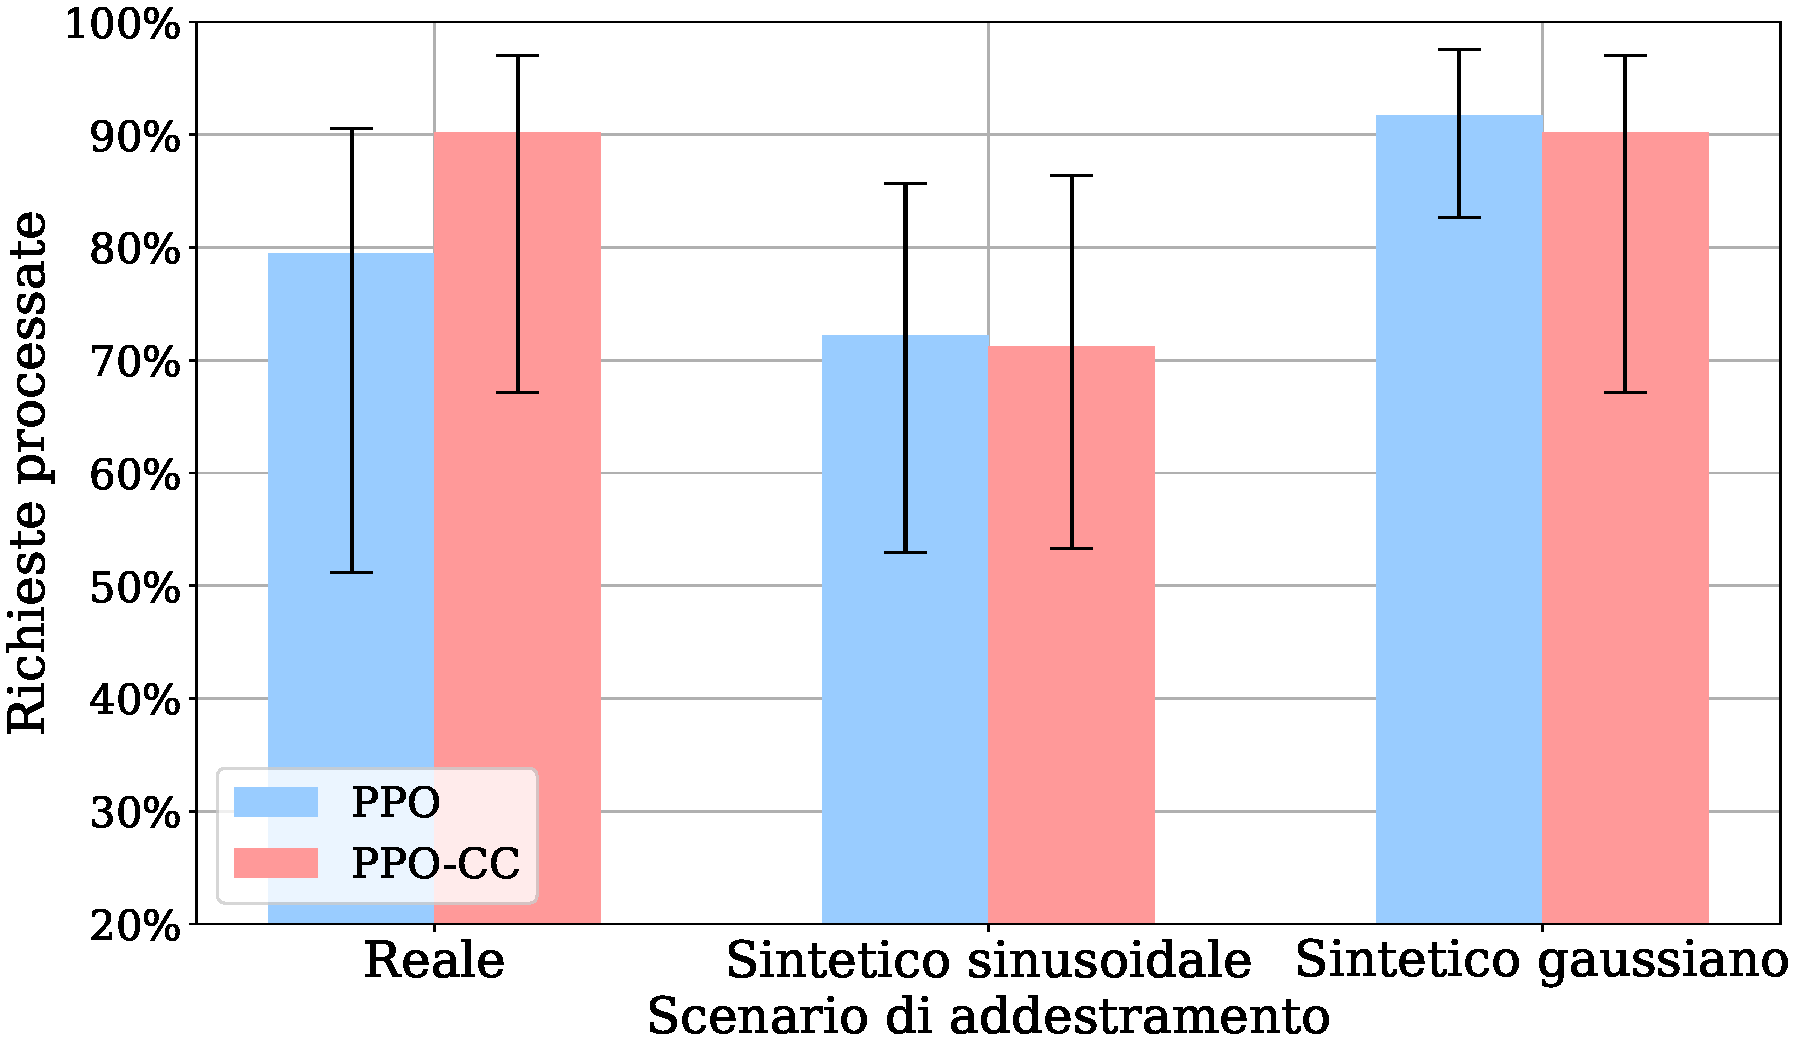
\includegraphics[width=\linewidth]{assets/5/results/eval_ASYM_summary_processed_requests.pdf}
        \caption{Ambiente ``ASYM''.}
    \end{subfigure}
    
    \begin{subfigure}{.8\textwidth}
        \centering
        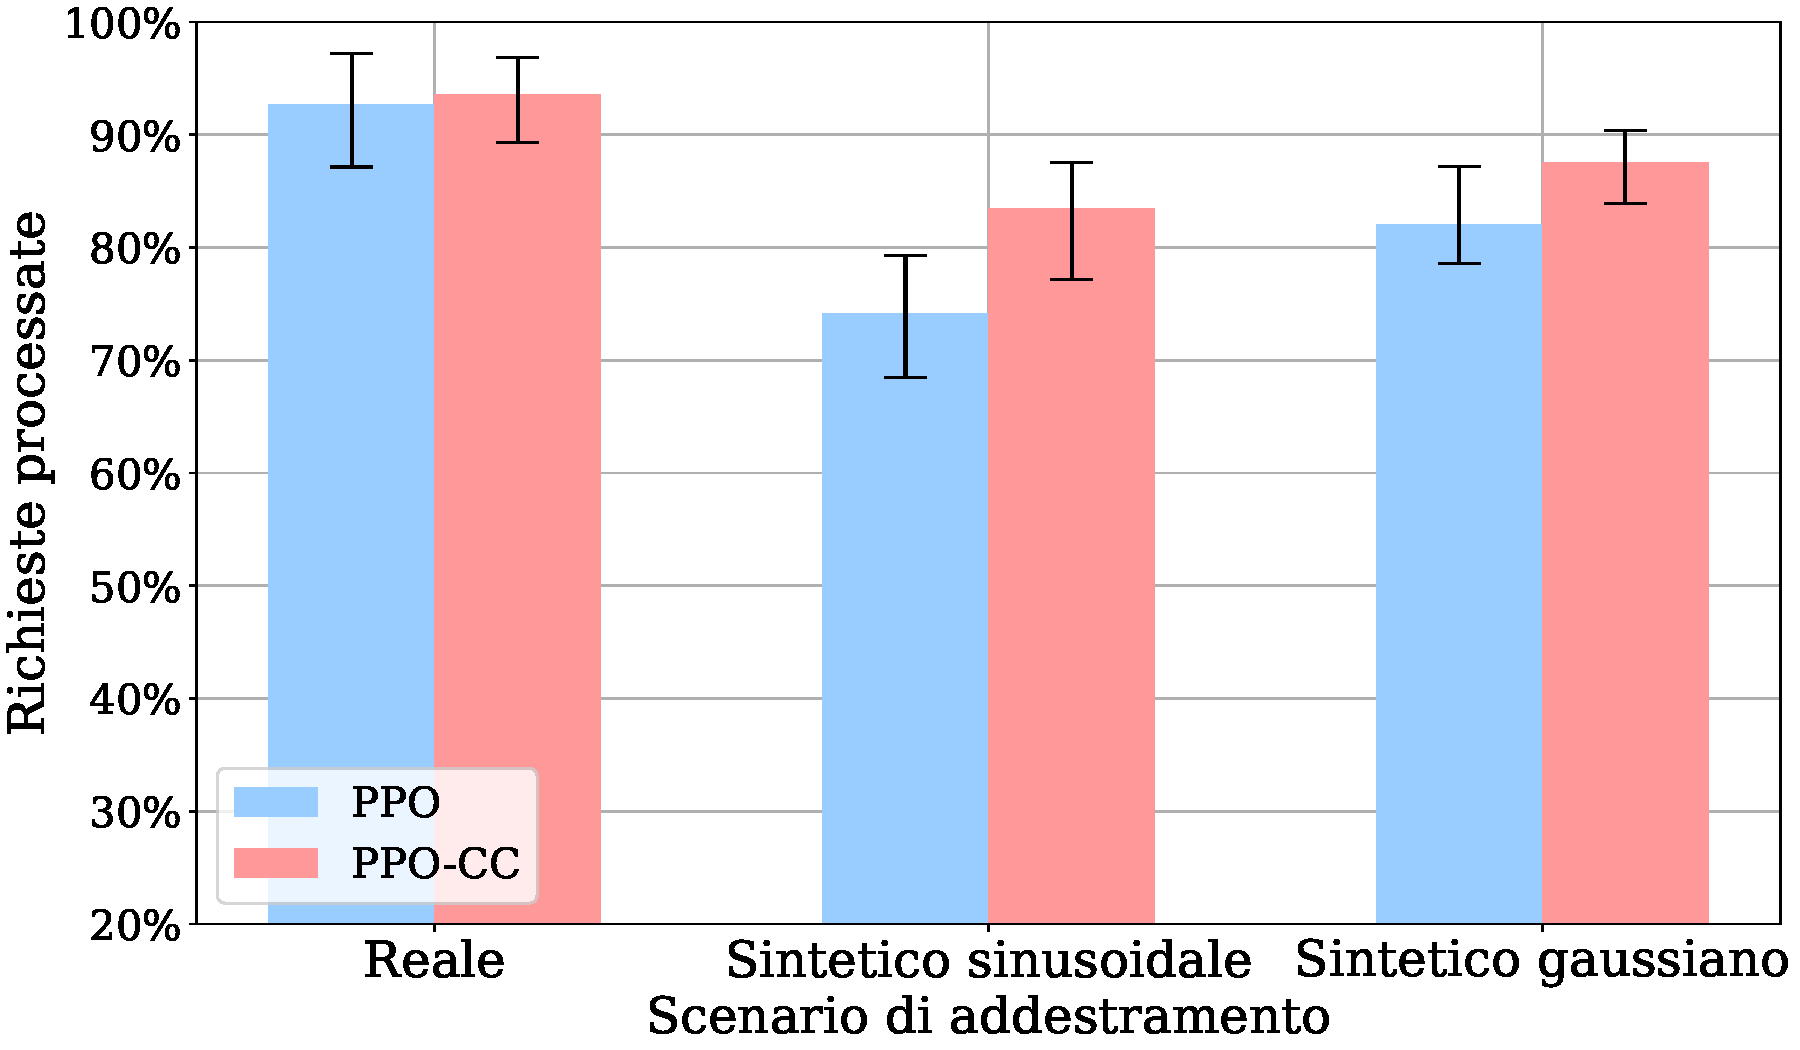
\includegraphics[width=\linewidth]{assets/5/results/eval_SYM_summary_processed_requests.pdf}
        \caption{Ambiente ``SYM''.}
    \end{subfigure}
    
    \caption[Media delle richieste processate nelle valutazioni (percentuale)]{Percentuale media di richieste processate su tutte le valutazioni con valori di minimo e massimo (in nero). La percentuale è sul massimo numero di richieste processabili per episodio.}
    \label{fig:5_results_requests}
\end{figure}

Il migliore risultato lo ottengono gli agenti addestrati nell'ambiente simmetrico con inoltro sullo scenario reale, superando in media il 90\% delle richieste processabili. In \Cref{fig:5_eval_sym_train_real_requests} mostra in dettaglio le valutazioni su questo esperimento, mostrando che gli agenti riescono a generalizzare sui due scenari sintetici, oltre che sullo scenario reale di addestramento.

\begin{figure}
    \centering
    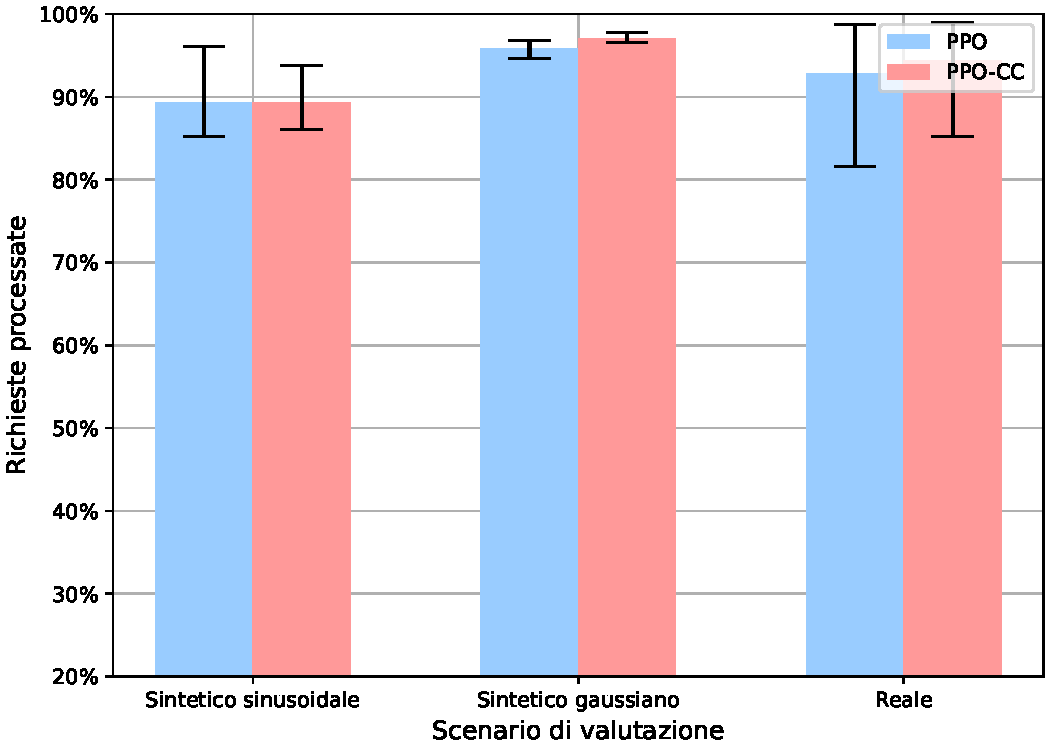
\includegraphics[width=.6\linewidth]{assets/5/results/eval_SYM_train_real_processed_requests.pdf}
    \caption[Richieste processate dagli agenti in ambiente SYM addestrati nello scenario reale]{Richieste processate dagli agenti in ambiente SYM addestrati nello scenario reale. In nero sono i valori di minimo e massimo. La percentuale è sul massimo numero di richieste processabili per episodio.}
    \label{fig:5_eval_sym_train_real_requests}
\end{figure}

I tre scenari sono stati progettati per avere difficoltà diversa:

\begin{itemize}
    \item Lo scenario gaussiano è il più semplice, perché le richieste in arrivo variano intorno a un valore medio. Ciò viene confermato dai risultati negli ambienti asimmetrico e simmetrico senza inoltro. Per l'ambiente simmetrico, ottiene delle prestazioni inferiori rispetto allo scenario reale, come mostrato in \Cref{fig:5_eval_sym_train_normal_requests}. Questo perché gli agenti non riesco a generalizzare e ottengono addirittura un risultato peggiore rispetto agli agenti addestrati in scenario reale e valutati su scenario gaussiano.

    \item Lo scenario sinusoidale risulta essere il più difficile da gestire: le tracce in ingresso possono essere in fase e rendere difficile il lavoro agli agenti, poiché entrambi saranno impossibilitati a processare le richieste localmente o ad inoltrarle. Un inoltro eccessivo può infatti portare a un peggioramento delle prestazioni. Negli ambienti asimmetrici e simmetrici con inoltro, la possibilità di inoltrare può essere controproducente in questi casi, come mostrato in \Cref{fig:5_results_requests}

    \item Lo scenario reale è l'unico che presenta una crescita delle richieste processate all'aumentare della complessità degli ambienti. Per via della forma delle tracce reali, gli agenti riescono a osservare molti casi e riescono a generalizzare la distribuzione del carico anche nei scenari sintetici. Inoltre in fase di valutazione le tracce reali sono estratte da un insieme di dati separato da quello di addestramento. 
\end{itemize}

\begin{figure}
    \centering
    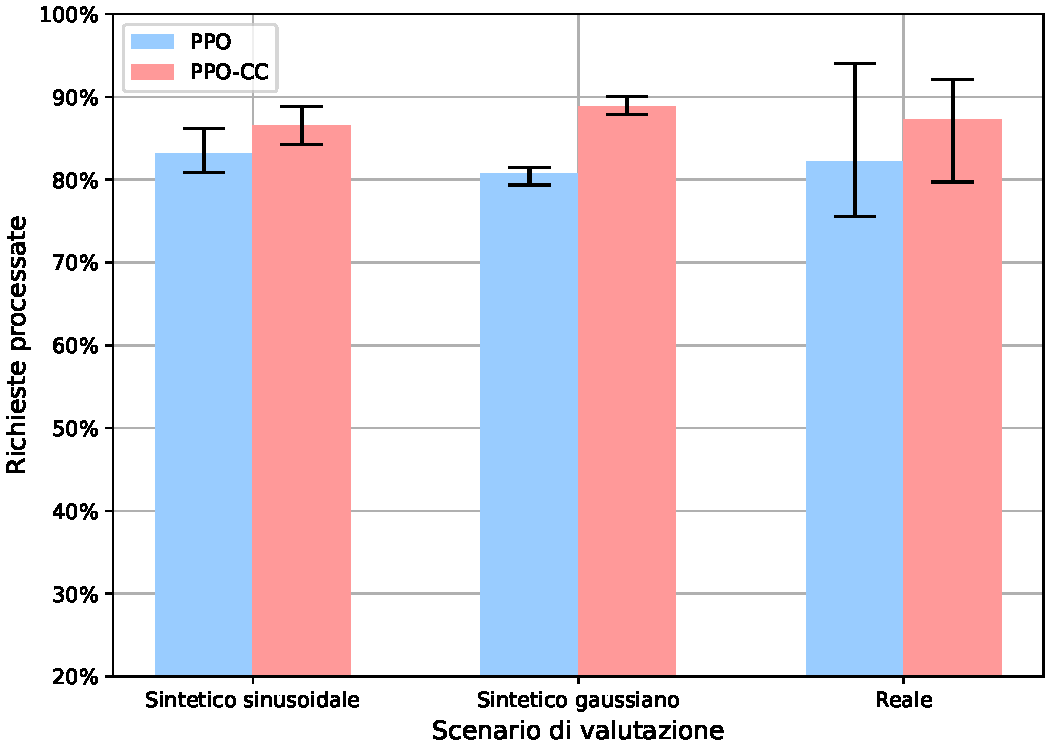
\includegraphics[width=.6\linewidth]{assets/5/results/eval_SYM_train_synthetic-normal_processed_requests.pdf}
    \caption[Richieste processate dagli agenti in ambiente SYM addestrati nello scenario gaussiano]{Richieste processate dagli agenti in ambiente SYM addestrati nello scenario gaussiano. In nero sono i valori di minimo e massimo. La percentuale è sul massimo numero di richieste processabili per episodio.}
    \label{fig:5_eval_sym_train_normal_requests}
\end{figure}

\paragraph{Influenza di PPO-CC.} L'addestramento centralizzato di PPO (PPO-CC) influisce in modo positivo sugli agenti nei tre ambienti e scenari con dei risultati pari o superiori, a eccezione dello scenario sinusoidale. In particolare nell'ambiente simmetrico con inoltro, gli agenti riescono a sfruttare al meglio la rete Critic condivisa per collaborare e processare più richieste, ottenendo pertanto un risultato migliore di PPO. Ciò non vale per gli altri due ambienti, in cui la capacità di inoltro degli agenti viene limitata, anzi porta un peggioramento in alcuni casi.

La \Cref{fig:5_sym_real_ppo_vs_ppo_cc} mostra la distribuzione delle richieste in valori assoluti per episodio tra PPO-CC e PPO, con gli agenti in ambiente simmetrico con inoltro, addestrati e valutati su scenario reale. Si può notare un sensibile aumento delle richieste inoltrate con PPO-CC rispetto a PPO.

\begin{figure}
    \centering

    \begin{subfigure}{.9\textwidth}
        \centering
        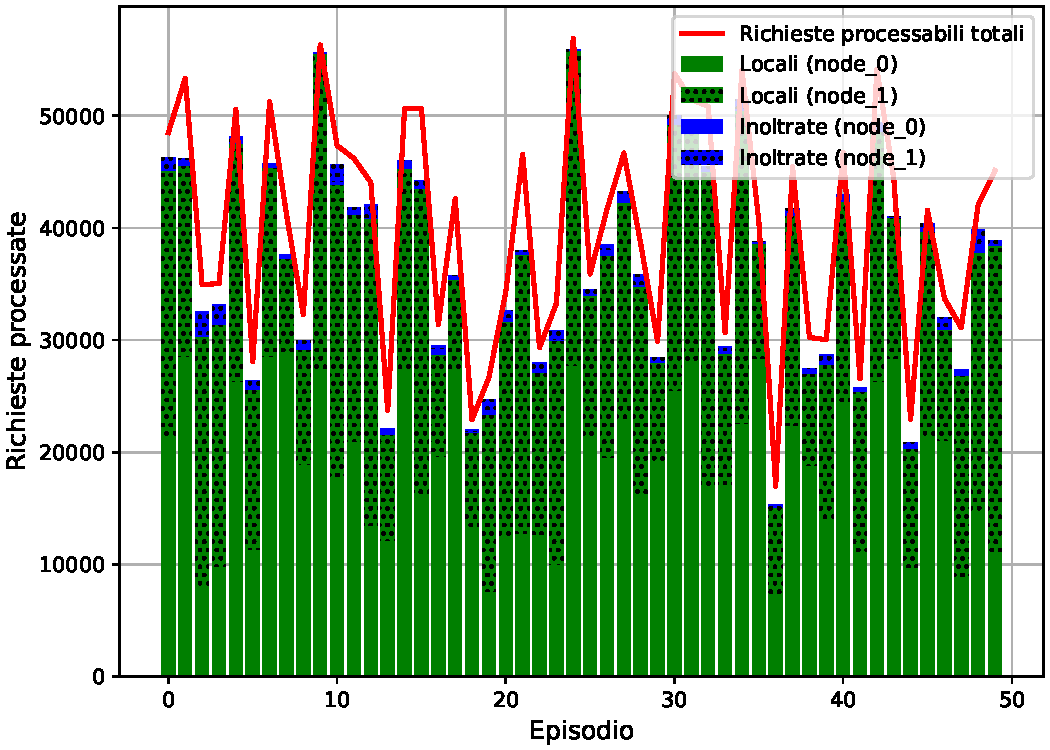
\includegraphics[width=\linewidth]{assets/5/results/real_real_ppo_proc_reqs_abs.pdf}
        \caption{PPO.}
    \end{subfigure}
    
    \begin{subfigure}{.9\textwidth}
        \centering
        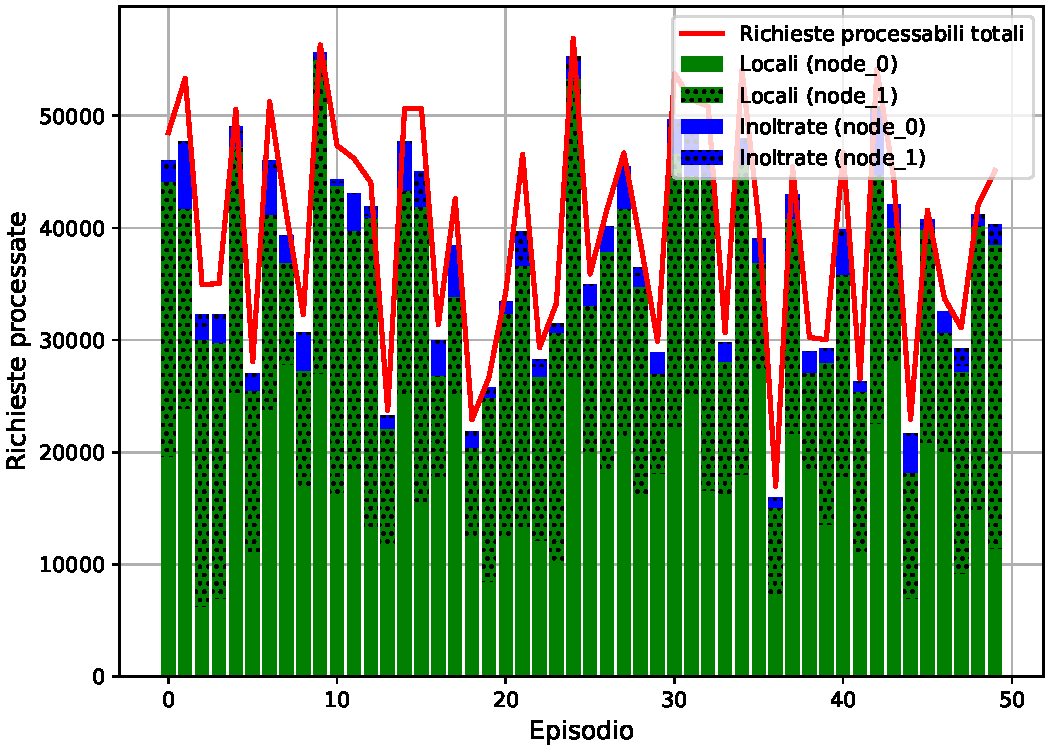
\includegraphics[width=\linewidth]{assets/5/results/real_real_ppo_cc_proc_reqs_abs.pdf}
        \caption{PPO-CC.}
    \end{subfigure}
    
    \caption[Distribuzione per episodio delle richieste in valore assoluti]{Distribuzione per episodio delle richieste con agenti in ambiente SYM, addestrati e valutati sullo scenario reale.}
    \label{fig:5_sym_real_ppo_vs_ppo_cc}
\end{figure}

\paragraph{} Rispondendo al quesito di ricerca RQ2, presentato nella \Cref{sec:1_obiettivi_ricerca}, i risultati ottenuti in questo capitolo indicano che l'approccio MARL può essere utilizzato per affrontare il problema della distribuzione del carico, al fine di processare più richieste possibili in un ambiente edge-FaaS. In particolare l'addestramento centralizzato ottiene prestazioni migliori rispetto all'addestramento decentralizzato nell'ambiente SYM, che è quello che più si avvicinare all'amiente DFaaS reale.

\chapter{Conclusioni}
\label{sec:6_conclusioni}

Quest'ultimo capitolo dell'elaborato contiene un sommario del lavoro svolto, evidenziando i risultati raggiunti, le limitazioni e le criticità affrontate, oltre che gli spunti per sviluppi futuri.

Nella \Cref{sec:1_obiettivi_ricerca} si sono descritti gli obiettivi di ricerca legati allo sviluppo di questa tesi: modellare un ambiente multi-agente per la gestione del carico in un sistema DFaaS e verificare che l'approccio multi-agente è in grado di affrontare questo problema. Partendo dalle basi teoriche riguardo le tematiche trattate nella tesi, presentate nel \Cref{sec:2_descrizione_contesto}, è stata svolta un'analisi dello stato nell'arte, nel \Cref{sec:3_stato_arte}, riscontrando l'assenza di lavori sulla incentrati sulla distribuzione del carico in ambienti edge-FaaS. Si è quindi iniziato a modellare un problema di RL multi-agente preliminare, nel \Cref{sec:4_modellazione}. A seguire sono stati creati ed eseguiti degli esperimenti in \Cref{sec:5_esperimenti}.

\paragraph{Risultati preliminari.} Un fattore importante nell'analisi dei risultati è la capacità degli agenti ad adattarsi in situazioni eterogenee, rappresentate dai diversi scenari di carico che abbiamo considerato. Sotto questa ottica, la migliore soluzione è stata ottenuta con gli agenti addestrati su uno scenario di carico reale, che riescono a processare oltre l'80\% delle richieste in ingresso sui tre scenari definiti, dimostrando che la possibilità di inoltrare parte delle richieste ai vicini ne migliora la gestione complessiva da parte del sistema. Nonostante non ci siano grosse differenza tra l'approccio MARL centralizzato e decentralizzato per la fase di addestramento, condividere la rete Critic aiuta gli agenti a scegliere azioni migliori rispetto l'assenza di condivisione.

\paragraph{Limitazioni e sviluppi futuri.} Sebbene il modello preliminare proposto rappresenti una notevole semplificazione del problema trattato, le difficoltà riscontrate e le osservazioni nate durante lo svolgimento della tesi hanno reso possibile individuare alcuni punti importanti per orientare futuri progetti:

\begin{itemize}
    \item Modellazione di un ambiente più complesso, in modo da avvicinarsi a una rappresentazione più vicina al sistema reale DFaaS. In particolare  si può lavorare sulla gestione delle richieste in coda, evitando che gli slot nella coda tornino tutti disponibili al passo successivo.

    \item Miglioramento della funzione di ricompensa in modo da incentivare la cooperazione tra agenti.

    \item Esplorazione più approfondita dell'approccio MARL al problema affrontato, sia nel determinare l'obiettivo degli agenti (un equilibrio comune o una massimizzazione locale) sia negli approcci di addestramento ed esecuzione. In particolare tra i problemi da affrontare ci sono: la non stazionarietà dell'ambiente, come assegnare la ricompensa e come scalare in ambienti con molti agenti.
    
    \item Tuning degli iperparametri: le scelte degli iperparametri in RL può influire molto sulle prestazioni degli agenti. In questa tesi sono stati utilizzati i valori predefiniti in RLlib, poiché gli obiettivi del lavoro erano concentrati sulla realizzabilità del modello e una prima sperimentazione. Tali iperparametri, per quanto scelti in modo da risultare funzionali in contesti generali, possono essere ottimizzati per lo specifico problema affrontato, in modo da ottenere prestazioni migliori.

    \item Approfondimento dell'approccio Deep Learning, al fine di costruire modelli di reti neurali più adatti al problema. Un limite attuale è l'uso delle reti neurali completamente connesse, non molto adatte in problemi in cui la sequenza degli eventi è rilevante, poiché le richieste in ingresso vicine sono correlate temporalmente. Reti con memoria, come le reti neurali ricorrenti (recurrent neural network, RNN), possono risultare più indicate per il problema affrontato.
\end{itemize}

\backmatter

\addcontentsline{toc}{chapter}{\protect\textbf{Elenco delle figure, tabelle e algoritmi}}
% The list of figures and tables in a single page.
{\listoffigures \let\cleardoublepage\null \listoftables \let\cleardoublepage\null \listofalgorithms}

\cleardoublepage

\printbibliography[title=Riferimenti bibliografici, heading=bibintoc]

\end{document}